%DIF 1c1
%DIF LATEXDIFF DIFFERENCE FILE
%DIF DEL PEARL_Chemoinfo.tex     Wed Nov 25 09:10:11 2026
%DIF ADD PEARL_ChemInfo_v5.tex   Wed Nov 25 09:10:09 2026
%DIF < \documentclass[pdflatex,sn-mathphys-num]{sn-jnl}% Basic Springer Nature Reference Style/Chemistry Reference Style (Journal of Cheminformatics)
%DIF -------
\documentclass[pdflatex,sn-mathphys-num,Numbered]{sn-jnl}%  Springer Nature Reference Style/Chemistry Reference Style (Journal of Cheminformatics), numbered citations %DIF > 
%DIF -------

\usepackage{graphicx}
\usepackage{multirow}
\usepackage{amsmath,amssymb,amsfonts}
\usepackage{booktabs}
%DIF 7a7
\usepackage{array} %DIF > 
%DIF -------
\usepackage{adjustbox}
%DIF 8a9-12
\usepackage{xcolor} %DIF > 
\usepackage{subcaption} %DIF > 
\usepackage{placeins} %DIF > 
\newcommand{\pending}[1]{{\color{red}\textbf{[PENDING: #1]}}}% result or check still to be filled in before submission %DIF > 
%DIF -------

%DIF 9c14-23
%DIF < %\graphicspath{{Figures_v2/}}
%DIF -------
% Wrapping text columns for the wide result tables, so they set at a readable size inside the %DIF > 
% text block instead of being shrunk to fit by \resizebox / \adjustbox. %DIF > 
\newcolumntype{L}[1]{>{\raggedright\arraybackslash}p{#1}} %DIF > 
\newcolumntype{C}[1]{>{\centering\arraybackslash}p{#1}} %DIF > 
 %DIF > 
\graphicspath{{Chemoinformatics_Revision/VERSION 5/Figures_v2/}{Chemoinformatics_Revision/VERSION 5/Figures_v3/}} %DIF > 
% generated by scripts/revision/build_response.py; do not edit
\newcommand{\mBACEFT}{0.542}
\newcommand{\sBACEFT}{0.005}
\newcommand{\srBACEFT}{0.557}
\newcommand{\cfgBACEFT}{MolFormer WL / XGBoost}
\newcommand{\mBACEFTPC}{0.549}
\newcommand{\sBACEFTPC}{0.020}
\newcommand{\srBACEFTPC}{0.550}
\newcommand{\cfgBACEFTPC}{MolFormer WL / LightGBM}
\newcommand{\mBACERAFE}{0.553}
\newcommand{\sBACERAFE}{0.017}
\newcommand{\srBACERAFE}{0.561}
\newcommand{\cfgBACERAFE}{MolFormer WL / LightGBM}
\newcommand{\mBBBPFT}{0.783}
\newcommand{\sBBBPFT}{0.010}
\newcommand{\srBBBPFT}{0.787}
\newcommand{\cfgBBBPFT}{MolFormer FL / XGBoost}
\newcommand{\mBBBPFTPC}{0.785}
\newcommand{\sBBBPFTPC}{0.016}
\newcommand{\srBBBPFTPC}{0.789}
\newcommand{\cfgBBBPFTPC}{MolFormer FL / XGBoost}
\newcommand{\mBBBPRAFE}{0.779}
\newcommand{\sBBBPRAFE}{0.009}
\newcommand{\srBBBPRAFE}{0.798}
\newcommand{\cfgBBBPRAFE}{MolFormer FL / XGBoost}
\newcommand{\mCACOFT}{0.789}
\newcommand{\sCACOFT}{0.003}
\newcommand{\srCACOFT}{0.821}
\newcommand{\cfgCACOFT}{ChemBERTa-MTR Huber / LightGBM}
\newcommand{\mCACOFTPC}{0.819}
\newcommand{\sCACOFTPC}{0.006}
\newcommand{\srCACOFTPC}{0.827}
\newcommand{\cfgCACOFTPC}{ChemBERTa-MTR Huber / LightGBM}
\newcommand{\mCACORAFE}{0.817}
\newcommand{\sCACORAFE}{0.007}
\newcommand{\srCACORAFE}{0.835}
\newcommand{\cfgCACORAFE}{ChemBERTa-MTR Huber / XGBoost}
\newcommand{\mDILIFT}{0.613}
\newcommand{\sDILIFT}{0.047}
\newcommand{\srDILIFT}{0.673}
\newcommand{\cfgDILIFT}{ChemBERTa-MLM FL / LightGBM}
\newcommand{\mDILIFTPC}{0.693}
\newcommand{\sDILIFTPC}{0.019}
\newcommand{\srDILIFTPC}{0.703}
\newcommand{\cfgDILIFTPC}{Uni-Mol FL / XGBoost}
\newcommand{\mDILIRAFE}{0.697}
\newcommand{\sDILIRAFE}{0.008}
\newcommand{\srDILIRAFE}{0.790}
\newcommand{\cfgDILIRAFE}{Uni-Mol FL / XGBoost}
\newcommand{\mHLFT}{0.592}
\newcommand{\sHLFT}{0.021}
\newcommand{\srHLFT}{0.623}
\newcommand{\cfgHLFT}{MolFormer Huber / XGBoost}
\newcommand{\mHLFTPC}{0.595}
\newcommand{\sHLFTPC}{0.017}
\newcommand{\srHLFTPC}{0.593}
\newcommand{\cfgHLFTPC}{MolFormer Huber / XGBoost}
\newcommand{\mHLRAFE}{0.559}
\newcommand{\sHLRAFE}{0.024}
\newcommand{\srHLRAFE}{0.568}
\newcommand{\cfgHLRAFE}{MolFormer Huber / XGBoost}
\newcommand{\mBACEPC}{0.485}
\newcommand{\mBBBPPC}{0.733}
\newcommand{\mCACOPC}{0.834}
\newcommand{\mDILIPC}{0.672}
\newcommand{\mHLPC}{0.499}
\newcommand{\ntop}{5}
\newcommand{\nds}{5}
\newcommand{\mrankRAFE}{2.8}
\newcommand{\mrankFTPC}{2.2}
\newcommand{\mrankFT}{3.8}
\newcommand{\mrankPC}{4.4}
\newcommand{\srtop}{6}
\newcommand{\srmean}{2.3}
\newcommand{\medtop}{2}
\newcommand{\medmean}{4.1}
\newcommand{\medpc}{1.4}
\newcommand{\nmf}{9}
\newcommand{\nsr}{14}
\newcommand{\nsep}{1}
\newcommand{\nrows}{15}
\newcommand{\gaplo}{0.00}
\newcommand{\gaphi}{0.23}
\newcommand{\cvtop}{2}
\newcommand{\cvmean}{4.6}
\newcommand{\cvpcmean}{2.6}
\newcommand{\fracsmall}{85}
\newcommand{\ncellsabl}{72}
\newcommand{\nbig}{11}
\newcommand{\nkcomp}{49}
\newcommand{\nkexc}{2}
\newcommand{\bigcfg}{BACE, DILI, Half-Life}
\newcommand{\excdetails}{Flavor with LightGBM, CLM-cosine versus random neighbours (random higher by 0.010): $-$0.010, 95\% CI $-$0.018 to $-$0.000; Caco-2 with CatBoost, k100 versus k10: $-$0.008, 95\% CI $-$0.015 to $-$0.001}
\newcommand{\spmin}{$-$0.02}
\newcommand{\spmax}{+0.14}
\newcommand{\rgAlo}{36}
\newcommand{\rgAhi}{52}
\newcommand{\rgBlo}{47}
\newcommand{\rgBhi}{76}
\newcommand{\rgClo}{32}
\newcommand{\rgChi}{74}
\newcommand{\ecorrmax}{4}
\newcommand{\vn}{72}
\newcommand{\vbetterft}{1}
\newcommand{\vworseft}{7}
\newcommand{\vbetterrf}{0}
\newcommand{\vworserf}{0}
\newcommand{\covmedian}{0.40}
\newcommand{\covn}{34,018}
\newcommand{\covsixty}{5}
\newcommand{\covbace}{0.338}
\newcommand{\ecfpcaco}{0.607}
\newcommand{\pccaco}{0.838}
\newcommand{\draferecfpdili}{0.26}
\newcommand{\draferecfpcaco}{0.22}
\newcommand{\ecfpbace}{0.495}
\newcommand{\threedbace}{0.394}
\newcommand{\concatlo}{0.13}
\newcommand{\concathi}{0.14}
\newcommand{\coslo}{0.91}
\newcommand{\coshi}{0.92}
\newcommand{\rthreedlo}{4}
\newcommand{\rthreedhi}{7}
\newcommand{\rcatlo}{2}
\newcommand{\rcathi}{3}
\newcommand{\lorarun}{median 13 s, IQR 6-43 s, max 540 s}
\newcommand{\zhmin}{4.4}
\newcommand{\zdmin}{4.2}
\newcommand{\raferq}{0.13}
\newcommand{\umhours}{herg: 8.4 h, dili: 9.1 h, caco2: 1.7 h}
\newcommand{\bbbpcat}{+0.031}
\newcommand{\bbblgb}{+0.012}
\newcommand{\bbbxgb}{$-$0.006}
\newcommand{\dilirafecfg}{Uni-Mol FL with XGBoost}
\newcommand{\dilirafemcc}{0.790}
\newcommand{\dilirafeaucfg}{ChemBERTa-MLM FL with CatBoost}
\newcommand{\dilirafeauc}{0.907}
\newcommand{\rhomcclo}{0.65}
\newcommand{\rhomcchi}{0.79}
\newcommand{\sharethree}{57}
\newcommand{\rawr}{0.043}
\newcommand{\logr}{0.169}
\newcommand{\rhoall}{0.40}
\newcommand{\rhorafe}{0.25}
\newcommand{\spbestlo}{0.54}
\newcommand{\spbesthi}{0.62}
 %DIF > 
% Same values as tables/numbers.tex, with the dataset names spelled as they are everywhere else in %DIF > 
% the paper. Overridden here so the shared numbers file stays byte-identical for the earlier drafts. %DIF > 
\renewcommand{\umhours}{hERG 8.4 h, DILI 9.1 h, Caco-2 1.7 h} %DIF > 
%DIF -------

\raggedbottom
%DIF PREAMBLE EXTENSION ADDED BY LATEXDIFF
%DIF UNDERLINE PREAMBLE %DIF PREAMBLE
\RequirePackage[normalem]{ulem} %DIF PREAMBLE
\RequirePackage{color}\definecolor{RED}{rgb}{1,0,0}\definecolor{BLUE}{rgb}{0,0,1} %DIF PREAMBLE
\providecommand{\DIFadd}[1]{{\protect\color{blue}\uwave{#1}}} %DIF PREAMBLE
\providecommand{\DIFdel}[1]{{\protect\color{red}\sout{#1}}} %DIF PREAMBLE
%DIF SAFE PREAMBLE %DIF PREAMBLE
\providecommand{\DIFaddbegin}{} %DIF PREAMBLE
\providecommand{\DIFaddend}{} %DIF PREAMBLE
\providecommand{\DIFdelbegin}{} %DIF PREAMBLE
\providecommand{\DIFdelend}{} %DIF PREAMBLE
\providecommand{\DIFmodbegin}{} %DIF PREAMBLE
\providecommand{\DIFmodend}{} %DIF PREAMBLE
%DIF FLOATSAFE PREAMBLE %DIF PREAMBLE
\providecommand{\DIFaddFL}[1]{\DIFadd{#1}} %DIF PREAMBLE
\providecommand{\DIFdelFL}[1]{\DIFdel{#1}} %DIF PREAMBLE
\providecommand{\DIFaddbeginFL}{} %DIF PREAMBLE
\providecommand{\DIFaddendFL}{} %DIF PREAMBLE
\providecommand{\DIFdelbeginFL}{} %DIF PREAMBLE
\providecommand{\DIFdelendFL}{} %DIF PREAMBLE
\providecommand{\DIFscaledelfig}{0.5}
%DIF HIGHLIGHTGRAPHICS PREAMBLE %DIF PREAMBLE
\RequirePackage{settobox} %DIF PREAMBLE
\RequirePackage{letltxmacro} %DIF PREAMBLE
\newsavebox{\DIFdelgraphicsbox} %DIF PREAMBLE
\newlength{\DIFdelgraphicswidth} %DIF PREAMBLE
\newlength{\DIFdelgraphicsheight} %DIF PREAMBLE
% store original definition of \includegraphics %DIF PREAMBLE
\LetLtxMacro{\DIFOincludegraphics}{\includegraphics} %DIF PREAMBLE
\providecommand{\DIFaddincludegraphics}[2][]{{\color{blue}\fbox{\DIFOincludegraphics[#1]{#2}}}} %DIF PREAMBLE
\providecommand{\DIFdelincludegraphics}[2][]{% %DIF PREAMBLE
\sbox{\DIFdelgraphicsbox}{\DIFOincludegraphics[#1]{#2}}% %DIF PREAMBLE
\settoboxwidth{\DIFdelgraphicswidth}{\DIFdelgraphicsbox} %DIF PREAMBLE
\settoboxtotalheight{\DIFdelgraphicsheight}{\DIFdelgraphicsbox} %DIF PREAMBLE
\scalebox{\DIFscaledelfig}{% %DIF PREAMBLE
\parbox[b]{\DIFdelgraphicswidth}{\usebox{\DIFdelgraphicsbox}\\[-\baselineskip] \rule{\DIFdelgraphicswidth}{0em}}\llap{\resizebox{\DIFdelgraphicswidth}{\DIFdelgraphicsheight}{% %DIF PREAMBLE
\setlength{\unitlength}{\DIFdelgraphicswidth}% %DIF PREAMBLE
\begin{picture}(1,1)% %DIF PREAMBLE
\thicklines\linethickness{2pt} %DIF PREAMBLE
{\color[rgb]{1,0,0}\put(0,0){\framebox(1,1){}}}% %DIF PREAMBLE
{\color[rgb]{1,0,0}\put(0,0){\line( 1,1){1}}}% %DIF PREAMBLE
{\color[rgb]{1,0,0}\put(0,1){\line(1,-1){1}}}% %DIF PREAMBLE
\end{picture}% %DIF PREAMBLE
}\hspace*{3pt}}} %DIF PREAMBLE
} %DIF PREAMBLE
\LetLtxMacro{\DIFOaddbegin}{\DIFaddbegin} %DIF PREAMBLE
\LetLtxMacro{\DIFOaddend}{\DIFaddend} %DIF PREAMBLE
\LetLtxMacro{\DIFOdelbegin}{\DIFdelbegin} %DIF PREAMBLE
\LetLtxMacro{\DIFOdelend}{\DIFdelend} %DIF PREAMBLE
\DeclareRobustCommand{\DIFaddbegin}{\DIFOaddbegin \let\includegraphics\DIFaddincludegraphics} %DIF PREAMBLE
\DeclareRobustCommand{\DIFaddend}{\DIFOaddend \let\includegraphics\DIFOincludegraphics} %DIF PREAMBLE
\DeclareRobustCommand{\DIFdelbegin}{\DIFOdelbegin \let\includegraphics\DIFdelincludegraphics} %DIF PREAMBLE
\DeclareRobustCommand{\DIFdelend}{\DIFOaddend \let\includegraphics\DIFOincludegraphics} %DIF PREAMBLE
\LetLtxMacro{\DIFOaddbeginFL}{\DIFaddbeginFL} %DIF PREAMBLE
\LetLtxMacro{\DIFOaddendFL}{\DIFaddendFL} %DIF PREAMBLE
\LetLtxMacro{\DIFOdelbeginFL}{\DIFdelbeginFL} %DIF PREAMBLE
\LetLtxMacro{\DIFOdelendFL}{\DIFdelendFL} %DIF PREAMBLE
\DeclareRobustCommand{\DIFaddbeginFL}{\DIFOaddbeginFL \let\includegraphics\DIFaddincludegraphics} %DIF PREAMBLE
\DeclareRobustCommand{\DIFaddendFL}{\DIFOaddendFL \let\includegraphics\DIFOincludegraphics} %DIF PREAMBLE
\DeclareRobustCommand{\DIFdelbeginFL}{\DIFOdelbeginFL \let\includegraphics\DIFdelincludegraphics} %DIF PREAMBLE
\DeclareRobustCommand{\DIFdelendFL}{\DIFOaddendFL \let\includegraphics\DIFOincludegraphics} %DIF PREAMBLE
%DIF AMSMATHULEM PREAMBLE %DIF PREAMBLE
\makeatletter %DIF PREAMBLE
\let\sout@orig\sout %DIF PREAMBLE
\renewcommand{\sout}[1]{\ifmmode\text{\sout@orig{\ensuremath{#1}}}\else\sout@orig{#1}\fi} %DIF PREAMBLE
\makeatother %DIF PREAMBLE
%DIF COLORLISTINGS PREAMBLE %DIF PREAMBLE
\RequirePackage{listings} %DIF PREAMBLE
\RequirePackage{color} %DIF PREAMBLE
\lstdefinelanguage{DIFcode}{ %DIF PREAMBLE
%DIF DIFCODE_UNDERLINE %DIF PREAMBLE
  moredelim=[il][\color{red}\sout]{\%DIF\ <\ }, %DIF PREAMBLE
  moredelim=[il][\color{blue}\uwave]{\%DIF\ >\ } %DIF PREAMBLE
} %DIF PREAMBLE
\lstdefinestyle{DIFverbatimstyle}{ %DIF PREAMBLE
	language=DIFcode, %DIF PREAMBLE
	basicstyle=\ttfamily, %DIF PREAMBLE
	columns=fullflexible, %DIF PREAMBLE
	keepspaces=true %DIF PREAMBLE
} %DIF PREAMBLE
\lstnewenvironment{DIFverbatim}[1][]{\lstset{style=DIFverbatimstyle}}{} %DIF PREAMBLE
\lstnewenvironment{DIFverbatim*}[1][]{\lstset{style=DIFverbatimstyle,showspaces=true}}{} %DIF PREAMBLE
\lstset{extendedchars=\true,inputencoding=utf8}

%DIF END PREAMBLE EXTENSION ADDED BY LATEXDIFF

\begin{document}

\title[PEARL]{PEARL: Parameter-Efficient Adaptation with Retrieval-Augmented Learning for Molecular Property Prediction}

\author[1]{\fnm{Kavya} \sur{Agrawal}}
\author[1]{\fnm{Sukrit} \sur{Gupta}}
\author[2]{\fnm{Yundong} \sur{Zhou}}
\author[3]{\fnm{Chengliang} \sur{Yin}}
\author[4]{\fnm{Halima} \sur{Bensmail}}
\author*[4,5]{\fnm{Raghvendra} \sur{Mall}}\email{ramall@hbku.edu.qa, raghvendramall@ieee.org}

\affil[1]{\orgdiv{Center for Applied Research in Data Science}, \orgname{Indian Institute of Technology Ropar}, \orgaddress{\street{Rupnagar}, \postcode{140001}, \state{Punjab}, \country{India}}}

\DIFdelbegin %DIFDELCMD < \affil[2]{\orgdiv{The Second Department of Oncology, Cancer Center},
%DIFDELCMD < \orgname{Huizhou First Hosptial}, 
%DIFDELCMD < \orgaddress{\city{Huizhou}, \state{Guangdong},
%DIFDELCMD < \country{China}}}
%DIFDELCMD < %%%
\DIFdelend \DIFaddbegin \affil[2]{\orgdiv{The Second Department of Oncology, Cancer Center},
\orgname{Huizhou First Hospital}, 
\orgaddress{\city{Huizhou}, \state{Guangdong},
\country{China}}}
\DIFaddend 

\affil[3]{\orgdiv{Department of Biomedical Engineering},
\orgname{Faculty of Engineering, Universiti Malaya},
\orgaddress{\city{Kuala Lumpur}, \postcode{50603},
\country{Malaysia}}}

\affil*[4]{\orgdiv{Qatar Computing Research Institute},
\orgname{Hamad Bin Khalifa University},
\orgaddress{\city{Doha}, \country{Qatar}}}

\DIFdelbegin %DIFDELCMD < \affil*[5]{\orgdiv{Translational Medicine Department},
%DIFDELCMD < \orgname{Sidra Medicine},
%DIFDELCMD < \orgaddress{\city{Doha}, \country{Qatar}}}
%DIFDELCMD < %%%
\DIFdelend \DIFaddbegin \affil*[5]{\orgdiv{Translational Medicine},
\orgname{Sidra Medicine},
\orgaddress{\city{Doha}, \country{Qatar}}}
\DIFaddend 


\DIFdelbegin %DIFDELCMD < \abstract{
%DIFDELCMD < \textbf{Background}: Molecular property prediction sits at the center of computational drug discovery, and it hinges on a tension between two complementary views of a molecule: the sequential chemistry encoded in a SMILES string and the three-dimensional geometry that actually governs binding and toxicity. Yet no benchmark has directly compared parameter-efficient adaptation of 1D chemical language models (CLMs) against a SE(3)-equivariant 3D model across diverse molecular tasks and adaptation regimes - classification \emph{and} regression - while also controlling for a strong, non-CLM baseline built purely from engineered physicochemical (PC) descriptors and in-house graph neural networks (GNNs) evaluated under an identical protocol.\\
%DIFDELCMD < \textbf{Methods:} We introduce PEARL (\textbf{P}arameter-\textbf{E}fficient \textbf{A}daptation with \textbf{R}etrieval-augmented \textbf{L}earning). PEARL (i)~benchmarks Low-Rank Adaptation (LoRA) uniformly across three CLM families - ChemBERTa, MolFormer, and Uni-Mol - on seven molecular property datasets spanning binary classification, multi-class classification, and regression; (ii)~introduces a \textit{Retrieval-Augmented Feature Enhancement} (RAFE) pipeline that enriches predictions with label-free physicochemical neighborhood context from the ZINC-250k knowledge base; and 	(iii)~for every dataset, benchmarks a PC-only tree-ensemble baseline and in-house Chemprop and GCN models trained under the exact same scaffold splits and evaluation protocol as the CLM ladder.\\
%DIFDELCMD < \textbf{Results:} Uni-Mol's SE(3)-equivariant architecture achieves the best BACE inhibitor classification (MCC$=$0.623), an $8\%$ absolute gain over the best SMILES-based model, confirming that 3D geometry provides an inductive advantage for binding-affinity tasks. RAFE achieves the best overall result on \textbf{BBBP} (MolFormer, MCC$=$0.798) and, on the ADMET datasets, is the point-estimate winner on \textbf{DILI} (Uni-Mol RAFE, MCC$=$0.790). On all four ADMET datasets (hERG, DILI, Caco-2, Half-Life), however, the point-estimate winner's band overlaps the PC-only baseline's band - i.e.\ none of the four clears a statistically confirmed win over PC-only, extending a pattern already visible on the Flavor dataset. Taken together, these results show that LoRA-adapted CLMs and RAFE retrieval augmentation can match or exceed published full-finetuning and graph-based baselines (including GROVER-Large and Mole-BERT) while reducing trainable parameters by $76$-$97\%$. Still, a strong, non-neural PC-only baseline remains statistically competitive wherever task performance is not governed by 3D structure.\\
%DIFDELCMD < \textbf{Availability:} All code is publicly available at \url{https://github.com/raghvendra5688/PEARL}
%DIFDELCMD < }
%DIFDELCMD < %%%
\DIFdelend \DIFaddbegin \abstract{
\textbf{Background}: Molecular property prediction can start from a SMILES sequence or from three-dimensional geometry. Benchmarks rarely compare parameter-efficient adaptation of one-dimensional chemical language models (CLMs) with an SE(3)-equivariant 3D model across both task types, and seldom control for engineered physicochemical (PC) descriptors or for graph networks trained under the same protocol.\\
\textbf{Methods:} We introduce PEARL (\textbf{P}arameter-\textbf{E}fficient \textbf{A}daptation with \textbf{R}etrieval-augmented \textbf{L}earning). PEARL (i)~applies Low-Rank Adaptation (LoRA) to three CLM families (ChemBERTa, MolFormer, Uni-Mol) across seven classification and regression datasets; (ii)~adds a \textit{Retrieval-Augmented Feature Enhancement} (RAFE) stage, summarizing each molecule's ZINC-250k neighborhood with 60 label-free features; and (iii)~trains PC-only, fingerprint, Chemprop and GCN baselines in-house under the same scaffold splits. Every stage is run with three tree models (XGBoost, LightGBM, CatBoost), five seeds and training-split-only tuning, and differences are assessed with paired bootstrap intervals on identical test molecules.\\
\textbf{Results:} In matched comparisons, RAFE improves on the fine-tuned embedding alone on four of seven datasets (BBBP, hERG, DILI and Caco-2). Across 24 paired comparisons it is never significantly better or worse than embedding plus PC descriptors. The descriptor-only baseline is hard to beat: RAFE is significantly below it on hERG and Flavor and never significantly above it. Random ZINC-250k neighbors work as well as similar ones and the gain is unrelated to coverage, so RAFE acts as chemical-space context rather than analogue lookup. On five-seed means over the complete grid, the best RAFE configuration is top-three of seven methods on \ntop{} datasets (mean rank \mrankRAFE{}), with embedding plus descriptors (\mrankFTPC{}) and the descriptor baseline (\mrankPC{}) within half a rank. End-to-end LoRA on Uni-Mol gives the best BACE result (MCC$=$0.623, single run), but its frozen embedding is conformer-sensitive and contains an ECFP4 block. LoRA reduces the number of trainable parameters by $76$-$97\%$.\\
\textbf{Conclusions:} RAFE is an inexpensive final stage with dataset-specific value over a fine-tuned embedding and competitive with embedding plus descriptors. A PC-only baseline should be a standard control in CLM benchmarks.\\
\textbf{Availability:} All code is publicly available at \url{https://github.com/raghvendra5688/PEARL}
}
\DIFaddend 

\keywords{Retrieval-Augmented Generation, Parameter-Efficient Finetuning, Chemical Language Models, Low-Rank Adaptation, 3D Molecular Representations, ADMET Property Prediction, Computational Drug Discovery, Chemoinformatics}

\maketitle

%% =====================================================================
\section{Introduction}\label{sec:intro}

Understanding how molecular structure determines biological or physicochemical properties sits at the heart of computational drug discovery. Traditional quantitative structure-activity relationship (QSAR) methods lean on handcrafted molecular descriptors, but deep learning, and transformer-based architectures~\cite{vaswani2017attention} now let us learn molecular representations end-to-end directly from a molecule's Simplified Molecular Input Line Entry System (SMILES) sequence. That shift has driven the rise of chemical language models (CLMs) pretrained on enormous molecular corpora, which increasingly rival experimental approaches for predicting toxicity, solubility, and bioactivity~\cite{ahmad2022chemberta2,huang2020deeppurpose}.

Three problems, though, keep coming up. First, CLMs treat SMILES as flat token sequences, so they have no built-in notion of the three-dimensional geometry that governs binding affinity and enzyme inhibition. Second, fine-tuning an $\mathcal{O}(10^8)$-parameter CLM separately for each specialized task is often simply too expensive in resource-constrained settings. Third, and perhaps most avoidably, CLM benchmarking papers routinely compare against GNN baselines \emph{cited from other papers} rather than re-run under the same splits, preprocessing, and evaluation protocol, which makes a reported ``win'' hard to interpret causally.

Here we take on all three at once. We work with three model families: MolFormer~\cite{ross2022molformer}, ChemBERTa-2~\cite{ahmad2022chemberta2}, and Uni-Mol~\cite{zhou2023unimol}, the last a SE(3)-equivariant Transformer that operates directly on explicit 3D atomic coordinates, and apply Low-Rank Adaptation (LoRA)~\cite{hu2021lora} to each. On top of this, we build a \emph{Retrieval-Augmented Feature Enhancement} (RAFE) framework, which uses task-specific finetuned embeddings to pull the nearest chemical neighbors from ZINC-250k~\cite{gomez2018automatic}, a 249,455-molecule drug-like library, via GPU-accelerated FAISS indices~\cite{johnson2021faiss}. To close the third gap, for every one of the seven datasets we train Chemprop~\cite{yang2019chemprop} and a graph convolutional network (GCN) \emph{in-house}, under the same scaffold split and bootstrapped-CI evaluation protocol as every CLM-based method. Alongside these we add a \textbf{PC-only} baseline: a tree ensemble trained purely on 473 physicochemical (PC) descriptors, with no CLM embedding at all. \DIFdelbegin \DIFdel{That baseline suite is what lets us actually answer }\DIFdelend \DIFaddbegin \DIFadd{This baseline suite lets us ask }\DIFaddend whether the CLM ladder (End-to-End [E2E] LoRA, Finetune [FT] Embed, FT Embed+PC, RAFE) earns its added complexity over a simpler, non-neural alternative.

We \DIFdelbegin \DIFdel{benchmark }\DIFdelend \DIFaddbegin \DIFadd{also designed the study around a question that benchmark tables often leave open: does an apparent gain come from the representation or from the choice of tree model? Every stage of the ladder is therefore run with XGBoost, LightGBM and CatBoost, with the same tuning budget (20 Optuna trials, 5-fold cross-validation on the training split only) and five seeds. Differences are reported as paired bootstrap intervals on identical test molecules (Section~\ref{sec:eval_protocol}).
}

\DIFadd{We benchmark }\DIFaddend PEARL on seven molecular property prediction datasets: three MoleculeNet-era classification tasks, namely $\beta$-secretase inhibition (BACE), blood-brain-barrier prediction (BBBP), and flavor (Flavor) prediction. The other four come from the Therapeutics Data Commons (TDC) ADMET Group~\cite{huang2021tdc}: hERG cardiac-channel inhibition~\cite{wang2016herg}, drug-induced liver injury (DILI)~\cite{xu2019dili}, Caco-2 permeability (regression)~\cite{wang2016caco2}, and drug half-life (regression)~\cite{obach2008half}. Two of the seven are regression tasks, which means the PEARL ladder, RAFE, and every baseline all need to support Huber-loss finetuning and R\textsuperscript{2}/MAE/Spearman evaluation, described in Section~\ref{sec:pearl_arch}.

\DIFdelbegin \DIFdel{Our core contributions include}\DIFdelend \DIFaddbegin \DIFadd{We organize the study around three hypotheses. }\textbf{\DIFadd{H1:}} \DIFadd{LoRA adaptation is parameter-efficient without loss of accuracy. }\textbf{\DIFadd{H2:}} \DIFadd{retrieval features add information beyond the language-model embedding and the descriptors. }\textbf{\DIFadd{H3:}} \DIFadd{3D geometry helps structure-dependent endpoints. Section~\ref{sec:results_discussion} tests each in turn.
}

\DIFadd{Our contributions are}\DIFaddend :
\begin{itemize}
  \item \textbf{The PEARL framework\DIFaddbegin \DIFadd{.}\DIFaddend } \DIFdelbegin \DIFdel{, which unifies parameter-efficient LoRA adaptation across }\DIFdelend \DIFaddbegin \DIFadd{It combines LoRA adaptation of }\DIFaddend three CLM families (ChemBERTa, MolFormer, Uni-Mol) with \DIFdelbegin \DIFdel{a novel RAFEpipeline that injects }\DIFdelend \DIFaddbegin \DIFadd{RAFE, a retrieval stage that adds 60 }\DIFaddend label-free \DIFdelbegin \DIFdel{physicochemical neighborhood context }\DIFdelend \DIFaddbegin \DIFadd{neighborhood features computed }\DIFaddend from an external \DIFdelbegin \DIFdel{knowledge base }\DIFdelend \DIFaddbegin \DIFadd{library }\DIFaddend (ZINC-250k)\DIFdelbegin \DIFdel{, spanning both }\DIFdelend \DIFaddbegin \DIFadd{. It covers }\DIFaddend classification and regression\DIFdelbegin \DIFdel{tasks}\DIFdelend .
  \item \textbf{A \DIFdelbegin \DIFdel{systematic, }\DIFdelend uniform benchmark\DIFaddbegin \DIFadd{.}\DIFaddend } \DIFdelbegin \DIFdel{across all three CLM families and both 1D/3D representations, using seven molecular property datasets and an identical }\DIFdelend \DIFaddbegin \DIFadd{All seven datasets share one }\DIFaddend scaffold split, \DIFdelbegin \DIFdel{hyperparameter search budget , and bootstrapped-CI evaluation protocolfor every method, including in-house-retrained Chemprop, GCN, }\DIFdelend \DIFaddbegin \DIFadd{one tuning budget }\DIFaddend and \DIFdelbegin \DIFdel{PC-only baselines}\DIFdelend \DIFaddbegin \DIFadd{one evaluation protocol, including in-house PC-only, fingerprint, Chemprop and GCN baselines, three tree models and five seeds (Section~\ref{sec:main_results})}\DIFaddend .
  \item \textbf{\DIFdelbegin \DIFdel{Insights into whether retrieval augmentation substitutes for explicit 3D geometry}%DIFDELCMD < \MBLOCKRIGHTBRACE%%%
\DIFdel{: RAFE is the overall point-estimate winner on BBBP (MCC$=0.798$) and DILI (MCC$=0.790$), but only Uni-Mol's explicit 3D SE(3)-equivariant architecture clears the PC-only baseline by a statistically confirmed margin on BACE (MCC$=0.623$), indicating that }\DIFdelend \DIFaddbegin \DIFadd{A controlled analysis of what RAFE adds.}} \DIFadd{RAFE improves on the fine-tuned embedding alone on four of seven datasets and is never significantly better or worse than embedding plus descriptors in 24 paired comparisons. Feature-group ablations, random and Morgan-similarity retrieval, a neighbor-count sweep and }\DIFaddend label-free \DIFdelbegin \DIFdel{retrieval features narrow, without fully closing, the gap to explicit 3D structural information on tasks where binding geometry is mechanistically decisive}\DIFdelend \DIFaddbegin \DIFadd{variants indicate that it acts as chemical-space context (Section~\ref{sec:rafe_effectiveness})}\DIFaddend .
  \item \DIFaddbegin \textbf{\DIFadd{Evidence on 3D information.}} \DIFadd{End-to-end LoRA on Uni-Mol gives the best BACE result (MCC=$0.623$, single run). The frozen Uni-Mol vector contains an ECFP4 block and depends on the conformer, and we quantify both effects (Section~\ref{sec:3d_ecfp}).
  }\item \DIFaddend All code, including the TDC data-curation, RAFE, and in-house \DIFdelbegin \DIFdel{GNN }\DIFdelend baseline pipelines, is publicly available at \url{https://github.com/raghvendra5688/PEARL}.
\end{itemize}

Figure~\ref{fig:workflow} illustrates the complete PEARL workflow. The molecular dataset is processed by one of three CLM backbones. LoRA adapters augment only the attention projection layers, keeping all other pretrained weights frozen. For Uni-Mol, 3D conformers (SE(3)) are pre-generated via ETKDGv3 + MMFF94 and cached. The finetuned model provides both end-to-end predictions and task-specific embeddings. These embeddings are optionally concatenated with engineered PC features and with ZINC-250k RAFE features retrieved via FAISS indices, and the resulting feature vector is fed to Optuna-tuned tree-based classifiers or regressors.

\begin{figure*}[!ht]
  \centering
  \DIFdelbeginFL %DIFDELCMD < \includegraphics[width=0.99\textwidth]{ Figures_v2/PEARL_HM_Workflow_v2.pdf}
%DIFDELCMD <   %%%
\DIFdelendFL \DIFaddbeginFL \includegraphics[width=0.99\textwidth]{PEARL_HM_Workflow_v2.pdf}
  \DIFaddendFL \caption{PEARL workflow. Molecules are processed by one of three CLM families (ChemBERTa, MolFormer, Uni-Mol) with LoRA adapters. Task-specific embeddings are fused with molecular PC features and ZINC-250k retrieval features, then passed to tree-based classifiers/regressors. Uni-Mol \DIFdelbeginFL \DIFdelFL{additionally }\DIFdelendFL \DIFaddbeginFL \DIFaddFL{also }\DIFaddendFL encodes 3D ETKDGv3 conformers via \DIFaddbeginFL \DIFaddFL{an }\DIFaddendFL SE(3) representation. The ladder spans both classification and regression targets (including Caco-2, Half-Life) and is benchmarked against in-house Chemprop/GCN/PC-only baselines run under the same protocol.}
  \label{fig:workflow}
\end{figure*}

%% =====================================================================
\section{Related Work}\label{sec:related_work}

\subsection{Molecular Property Prediction}\label{sec:related_mpp}
ChemBERTa~\cite{chithrananda2020chemberta} and ChemBERTa-2~\cite{ahmad2022chemberta2} adapted BERT-style masked language modelling to SMILES, establishing the template for CLM pretraining on large molecular corpora. MolFormer~\cite{ross2022molformer} scaled this to $1.1\times10^9$ molecules using linear attention. Uni-Mol~\cite{zhou2023unimol} departed from SMILES by operating on explicit 3D atomic coordinates via an SE(3)-equivariant transformer, achieving state-of-the-art results on MoleculeNet through full finetuning. Multi-modal models such as MolT5~\cite{edwards2022molt5}, nach0~\cite{livne2024nach0}, and Omni-Mol~\cite{hu2025omnimol} \DIFdelbegin \DIFdel{further }\DIFdelend integrate SMILES, graphs, and natural language, but systematic evaluation under parameter-efficient conditions remains limited. \DIFaddbegin \DIFadd{Other work adds geometric or chemical knowledge to the representation. GEM~\mbox{%DIFAUXCMD
\cite{fang2022geometry} }\hskip0pt%DIFAUXCMD
encodes bond lengths and angles in a geometry-enhanced graph network. KPGT~\mbox{%DIFAUXCMD
\cite{li2023kpgt} }\hskip0pt%DIFAUXCMD
pretrains a graph transformer with knowledge-guided molecular descriptors. LiTENexus~\mbox{%DIFAUXCMD
\cite{su2026litenexus} }\hskip0pt%DIFAUXCMD
injects quantum-chemical information into a physics-informed operator, and a recent survey and benchmark~\mbox{%DIFAUXCMD
\cite{li2026survey} }\hskip0pt%DIFAUXCMD
compares deep-learning approaches to property prediction in the foundation-model era. These studies change the representation or the pretraining objective. PEARL instead keeps the pretrained models fixed except for low-rank adapters and asks how much extra information, such as descriptors or a retrieved neighborhood, helps a downstream tree model.
}\DIFaddend 

On the graph side, Chemprop~\cite{yang2019chemprop}, AttentiveFP~\cite{xiong2020attentivefp}, GROVER~\cite{rong2020grover}, and Mole-BERT~\cite{xia2023molecbert} all show how much graph-based molecular representations can offer. \DIFdelbegin \DIFdel{Rather than }\DIFdelend \DIFaddbegin \DIFadd{Instead of }\DIFaddend taking those numbers \DIFdelbegin \DIFdel{as reported in }\DIFdelend \DIFaddbegin \DIFadd{from }\DIFaddend the original papers (Supplementary Section~S5), \textbf{PEARL \DIFdelbegin \DIFdel{additionally }\DIFdelend re-trains Chemprop and a GCN in-house\DIFdelbegin %DIFDELCMD < \MBLOCKRIGHTBRACE%%%
\DIFdel{, on the exact }\DIFdelend \DIFaddbegin } \DIFadd{on all seven datasets, with the }\DIFaddend same scaffold split, preprocessing \DIFdelbegin \DIFdel{, and bootstrapped-CI (confidence interval) }\DIFdelend \DIFaddbegin \DIFadd{and evaluation }\DIFaddend protocol as every other method\DIFdelbegin \DIFdel{, on all seven datasets}\DIFdelend . The TDC~\cite{huang2021tdc} ADMET Group provides curated, leaderboard-tracked hERG~\cite{wang2016herg}, DILI~\cite{xu2019dili}, Caco-2~\cite{wang2016caco2}, and half-life~\cite{obach2008half} datasets, which broaden PEARL beyond MoleculeNet-era classification tasks and include regression targets.

\subsection{Parameter-Efficient Fine-Tuning (PEFT)}\label{sec:related_peft}
LoRA~\cite{hu2021lora} introduced low-rank weight updates for large language models; PEFT methods have since been evaluated for molecular tasks. Balne et al.~\cite{balne2024peft} and Xu et al.~\cite{xu2023peftreview} survey PEFT strategies broadly, including adapter layers, prefix tuning, and LoRA, while Fu et al.~\cite{fu2023effectiveness} assess their effectiveness in NLP. The work closest to ours is EffiChem~\cite{harod2025effichem}, which shows that LoRA-based adaptation of 1D CLMs (ChemBERTa, MolFormer) can be efficient for molecular property prediction.

PEARL \DIFdelbegin \DIFdel{goes considerably further along three axes}\DIFdelend \DIFaddbegin \DIFadd{extends this work in three ways}\DIFaddend . First, it adds Uni-Mol, a 3D SE(3)-equivariant model, \DIFdelbegin \DIFdel{enabling the first direct LoRA comparison between }\DIFdelend \DIFaddbegin \DIFadd{and compares }\DIFaddend 1D SMILES-based and 3D geometry-aware CLMs \DIFaddbegin \DIFadd{under LoRA }\DIFaddend on identical scaffold splits. Second, it \DIFdelbegin \DIFdel{introduces the RAFEframework}\DIFdelend \DIFaddbegin \DIFadd{adds RAFE}\DIFaddend , which augments frozen CLM embeddings with label-free \DIFdelbegin \DIFdel{chemical }\DIFdelend neighborhood features from an external \DIFdelbegin \DIFdel{knowledge base}\DIFdelend \DIFaddbegin \DIFadd{library}\DIFaddend . Third, it \DIFdelbegin \DIFdel{benchmarks }\DIFdelend \DIFaddbegin \DIFadd{trains }\DIFaddend in-house GNN\DIFaddbegin \DIFadd{, fingerprint }\DIFaddend and PC-only baselines and extends the ladder to regression tasks. \DIFdelbegin \DIFdel{To our knowledge, no prior work combines PEFT with leakage-free retrieval augmentation across both 1D and 3D molecular representations and classification/regression tasks, under a fully in-house, identically-evaluated baseline suite}\DIFdelend \DIFaddbegin \DIFadd{We did not find a prior study that combines these elements under one protocol}\DIFaddend .

\subsection{Retrieval-Augmented Generation (RAG)}\label{sec:related_rag}
Generative RAG~\cite{lewis2020rag} conditions a language model on retrieved documents; molecular analogues typically retrieve labeled training-set molecules as auxiliary signals, introducing leakage and a small retrieval pool. KPGT~\cite{liu2022kpgt} injects knowledge-graph attributes into graph-transformer pretraining but retrieval occurs at pretraining time from the training corpus itself. \DIFdelbegin \DIFdel{PEARL's RAFE differs : it }\DIFdelend \DIFaddbegin \DIFadd{RAFE differs in three ways. It }\DIFaddend retrieves from a fixed external corpus (ZINC-250k) at inference time\DIFdelbegin \DIFdel{, }\DIFdelend \DIFaddbegin \DIFadd{. It }\DIFaddend extracts label-free physicochemical statistics as tree-model features\DIFdelbegin \DIFdel{, and }\DIFdelend \DIFaddbegin \DIFadd{. It }\DIFaddend applies to any CLM family without retraining.

%% =====================================================================
\section{Materials and Methods}\label{sec:pearl_arch}
This section describes the seven benchmark datasets, the three CLM backbones that the PEARL framework builds on, and the two mechanisms \DIFdelbegin \DIFdel{- }\DIFdelend \DIFaddbegin \DIFadd{that PEARL adds: }\DIFaddend parameter-efficient LoRA adaptation and RAFE retrieval augmentation. \DIFdelbegin \DIFdel{These together }\DIFdelend \DIFaddbegin \DIFadd{Together they }\DIFaddend define how PEARL adapts and enriches th\DIFdelbegin \DIFdel{os}\DIFdelend e backbones for downstream \DIFdelbegin \DIFdel{molecular }\DIFdelend property prediction.

\subsection{Datasets}\label{sec:datasets}
PEARL is evaluated on seven molecular property prediction datasets that, taken together, span binary classification, multi-class classification, and regression, and range in size from a few hundred to over fifteen thousand compounds (Table~\ref{tab:dataset_summary}). Three are MoleculeNet-era classification benchmarks; the remaining four come from the TDC ADMET Group and add regression targets and a different (70:10:20) split convention, described below.

The \textbf{Blood-Brain Barrier Penetration (BBBP)} dataset was originally curated in~\cite{martins2012bayesian} for predicting barrier permeability and contains over $2,000$ compounds with binary labels, integrated into the MoleculeNet~\cite{wu2018moleculenet} benchmark. Blood-brain barrier permeability is a standard early filter in CNS drug discovery, and BBBP's compounds and splits are sourced directly from the IBM MolFormer repository, where they underwent validity checks, duplicate removal, and class-ambiguity filtering before we used them.

The \textbf{Flavor Analysis and Recognition Transformer (FART)} dataset, introduced in~\cite{zimmermann2024fart}, is a multi-class taste prediction corpus of 15,025 compounds annotated as \textit{bitter}, \textit{sour}, \textit{sweet}, \textit{umami}, and \textit{undefined}. It is, by a wide margin, the largest and most class-imbalanced dataset in this study, and is the only multi-class task PEARL is benchmarked on.

The \textbf{BACE} dataset is part of MoleculeNet~\cite{wu2018moleculenet} and contains experimentally measured binding results for 1,513 inhibitors of human $\beta$-secretase~1 (BACE-1), with binary activity labels. For all three of these MoleculeNet-era datasets, splits were curated using the DeepChem reference implementation~\cite{ramsundar2019deep}, which we use as-is rather than re-splitting the data ourselves, so that results remain comparable to prior work reporting on the same splits.

\textbf{TDC ADMET Group datasets:} Four datasets come from the Therapeutics Data Commons (TDC) ADMET Group~\cite{huang2021tdc}, chosen to broaden PEARL's task coverage beyond MoleculeNet-era binary/multi-class classification and to add regression targets. These include \textbf{hERG}~\cite{wang2016herg} (binary, cardiac ion-channel inhibition, 13{,}445 compounds), \textbf{DILI}~\cite{xu2019dili} (binary, drug-induced liver injury, 475 compounds), \textbf{Caco-2}~\cite{wang2016caco2} (regression, log apparent permeability, 906 compounds), and \textbf{Half-Life}~\cite{obach2008half} (regression, plasma half-life in hours, 667 compounds). All four are curated via TDC's standard scaffold split and undergo the same SMILES standardization, validity filtering, and duplicate-removal pipeline used for BACE, BBBP, and Flavor, so that no dataset in this study receives a bespoke preprocessing pipeline that could bias comparisons across the ladder. Half-Life \DIFdelbegin \DIFdel{additionally }\DIFdelend \DIFaddbegin \DIFadd{also }\DIFaddend required IQR-based outlier removal in log1p space (bounds fit on the training split only, applied to all splits)\DIFdelbegin \DIFdel{to control the influence of a small number of extreme half-life values (max }\DIFdelend \DIFaddbegin \DIFadd{. Without it, a handful of extreme values (maximum }\DIFaddend $\approx 1200$h \DIFdelbegin \DIFdel{vs.\ a }\DIFdelend \DIFaddbegin \DIFadd{against a mean of }\DIFaddend $\sim$19h \DIFdelbegin \DIFdel{mean pre-filtering) -- without which a handful of outlier compounds would otherwise }\DIFdelend \DIFaddbegin \DIFadd{before filtering) would }\DIFaddend dominate the regression loss.

\subsubsection{Data Splits and Class Distribution}\label{sec:data_splits}
BBBP and BACE employ scaffold-based splits~\cite{ramsundar2019deep} using an 80:10:10 train/validation/test ratio. BBBP exhibits moderate class imbalance (78.8\% permeable in training); BACE is the most balanced dataset in this study, with $54.3\%$ inactive and $45.7\%$ active compounds, and its test set has $n\approx152$ molecules. The Flavor dataset uses the curated splits provided in~\cite{zimmermann2024fart}, with pronounced multi-class skew (sweet $41\%$, bitter $32\%$, sour $11\%$, umami $4\%$, undefined $12\%$) and $n_\text{test}=2{,}254$.

The four TDC ADMET datasets instead use TDC's scaffold split (70:10:20 train/valid/test, the TDC ADMET Group default). hERG's test set ($n=2{,}690$) is class-imbalanced toward inhibitors ($\sim$70\%); DILI is the smallest classification dataset in this study ($n_\text{test}=96$), so its bootstrapped CIs are correspondingly the widest among the binary tasks; Caco-2 ($n_\text{test}=182$) and Half-Life ($n_\text{test}=133$) are both small regression sets, motivating the same bootstrapped-CI discipline applied throughout this study.

\begin{table*}[!ht]
\centering
\caption{Structural summary of the seven PEARL benchmark datasets.}
\label{tab:dataset_summary}
\resizebox{0.9\textwidth}{!}{
\begin{tabular}{lllll}
\toprule
Dataset & Task type & \# Compounds & Split (train:val:test) & Primary metric \\
\midrule
BACE       & Binary classification       & 1{,}513  & 80:10:10 ($n_\text{test}\approx152$)   & MCC \\
BBBP       & Binary classification       & $>$2{,}000 & 80:10:10                               & MCC \\
Flavor     & 5-class classification      & 15{,}025 & curated~\cite{zimmermann2024fart} ($n_\text{test}=2{,}254$) & MCC \\
hERG       & Binary classification       & 13{,}445 & 70:10:20 ($n_\text{test}=2{,}690$)      & MCC \\
DILI       & Binary classification       & 475      & 70:10:20 ($n_\text{test}=96$)           & MCC \\
Caco-2     & Regression (log permeability) & 906    & 70:10:20 ($n_\text{test}=182$)          & Spearman \\
Half-Life  & Regression (log1p, hours)   & 667      & 70:10:20 ($n_\text{test}=133$)          & Spearman \\
\bottomrule
\end{tabular}
}
\end{table*}

\subsection{Problem Formulation}\label{sec:problem_formulation}
Let $\mathcal{D} = \{(x_i, y_i)\}_{i=1}^{N}$ denote a molecular property dataset, where $x_i$ is the $i$-th molecule \DIFdelbegin \DIFdel{-- }\DIFdelend \DIFaddbegin \DIFadd{and $y_i$ is its task-specific label. A molecule is }\DIFaddend represented either as a SMILES string (ChemBERTa, MolFormer) or \DIFaddbegin \DIFadd{as }\DIFaddend an explicit 3D atomic coordinate set obtained via conformer generation (Uni-Mol)\DIFdelbegin \DIFdel{-- and $y_i$ is its task-specific label}\DIFdelend . For binary classification tasks (BACE, BBBP, hERG, DILI), $y_i \in \{0,1\}$; for the multi-class Flavor task, $y_i \in \{1,\dots,5\}$; for regression tasks (Caco-2, Half-Life), $y_i \in \mathbb{R}$.

A pretrained CLM backbone $f_\theta : \mathcal{X} \rightarrow \mathbb{R}^{d}$ maps a molecule to a $d$-dimensional embedding ($d=384$ for ChemBERTa, $d=768$ for MolFormer, $d=2560$ for Uni-Mol's hybrid vector). PEARL learns a task-specific predictor $g_\phi$ such that
\begin{equation}
  \hat{y}_i = g_\phi\big(h(x_i)\big), \qquad h(x_i) = f_\theta(x_i) \,\Vert\, p(x_i) \,\Vert\, r(x_i),
\end{equation}
where $\Vert$ denotes concatenation, $p(x_i) \in \mathbb{R}^{473}$ is an optional vector of engineered physicochemical descriptors, and \DIFdelbegin \DIFdel{$r(x_i) \in \mathbb{R}^{69}$ }\DIFdelend \DIFaddbegin \DIFadd{$r(x_i) \in \mathbb{R}^{60}$ }\DIFaddend is an optional RAFE feature vector obtained by retrieving the $k$ nearest neighbors of $x_i$ in an external corpus $\mathcal{Z}$ (ZINC-250k). $\theta$ is adapted parameter-efficiently via low-rank updates $\Delta\theta$ with $|\Delta\theta| \ll |\theta|$, and $\phi$ is optimized to minimize a task-appropriate loss $\mathcal{L}(\hat y_i, y_i)$\DIFdelbegin \DIFdel{-- }\DIFdelend \DIFaddbegin \DIFadd{: }\DIFaddend weighted cross-entropy or focal loss for classification, Huber loss for regression. PEARL's four operational modes, described next, correspond to different choices of which terms in $h(x_i)$ are active and whether $g_\phi$ is trained end-to-end with $f_\theta$ or on frozen embeddings.

\subsection{Base CLM Backbone Architecture}\label{sec:pretrained_clms}
\textbf{ChemBERTa-2}~\cite{ahmad2022chemberta2} builds upon ChemBERTa~\cite{chithrananda2020chemberta} via a RoBERTa-style architecture trained on $77$ million canonical SMILES from PubChem~\cite{kim2023pubchem}. Two pretraining strategies are used: Masked Language Modeling (MLM) and Multi-Task Regression (MTR) on $200$ molecular property tasks. We use the two 77M-parameter variants, denoted \textbf{ChemBERTa-77M~MLM} and \textbf{ChemBERTa-77M~MTR}, each producing 384-dimensional embeddings.

\textbf{MolFormer}~\cite{ross2022molformer} is a scalable CLM that learns representations from SMILES without 3D geometry. It uses a transformer with linear attention (FAVOR+)~\cite{choromanski2021rethinking}, rotary positional embeddings~\cite{heo2024rotary}, and efficient distributed training~\cite{isard2009distributed}, enabling pretraining on $1.1\times 10^{9}$ molecules from PubChem~\cite{kim2023pubchem} and ZINC20~\cite{irwin2020zinc20}. We use the \textbf{MolFormer-XL-10pct-both} variant ($\approx 46$M parameters, pretrained on $10\%$ of both datasets) with 768-dimensional embeddings.

\textbf{Uni-Mol}~\cite{zhou2023unimol} is a universal 3D molecular pre-trained model based on a SE(3)-equivariant Transformer with 15 attention layers. Unlike SMILES-based CLMs, Uni-Mol accepts \emph{explicit 3D atomic coordinates} generated via RDKit ETKDGv3 conformer embedding followed by MMFF94 force-field minimization. This geometry-aware design gives Uni-Mol inductive biases suited to structure-dependent properties such as receptor binding affinity. For PEARL, each molecule is represented as a \textbf{2560-dimensional hybrid vector}: a 512-dimensional CLS token from the SE(3)-Transformer concatenated with 2048-dimensional Morgan ECFP4 fingerprints (radius $= 2$), combining 3D structural awareness with explicit 2D topological information.

\subsection{Parameter-Efficient Adaptation (LoRA)}\label{sec:lora}
Low-Rank Adaptation (LoRA)~\cite{hu2021lora} introduces two trainable low-rank matrices \DIFdelbegin \DIFdel{$\mathbf{A} \in \mathbb{R}^{d \times r}$ and $\mathbf{B} \in \mathbb{R}^{r \times d}$ }\DIFdelend \DIFaddbegin \DIFadd{$\mathbf{B} \in \mathbb{R}^{d \times r}$ and $\mathbf{A} \in \mathbb{R}^{r \times d}$ }\DIFaddend alongside frozen pretrained weight matrices $\mathbf{W} \in \mathbb{R}^{d \times d}$ in the attention layers, where $r \ll d$ is the rank hyperparameter. The weight update is:
\begin{equation}
  \mathbf{W}' = \mathbf{W} + \Delta\mathbf{W}, \quad \Delta\mathbf{W} = \DIFdelbegin \DIFdel{\mathbf{A} \cdot }\DIFdelend \DIFaddbegin \DIFadd{\frac{\alpha}{r}\,}\DIFaddend \mathbf{B}\DIFdelbegin \DIFdel{.
}\DIFdelend \DIFaddbegin \DIFadd{\mathbf{A},
}\DIFaddend \end{equation}
\DIFaddbegin \DIFadd{where $\alpha$ is the LoRA scaling factor. }\DIFaddend Matrix $\mathbf{A}$ is initialized \DIFdelbegin \DIFdel{from $\mathcal{N}(0, \sigma^2)$ }\DIFdelend \DIFaddbegin \DIFadd{with the Kaiming-uniform \mbox{%DIFAUXCMD
\cite{he2015delving} }\hskip0pt%DIFAUXCMD
scheme }\DIFaddend and $\mathbf{B}$ \DIFdelbegin \DIFdel{from zeros, ensuring that }\DIFdelend \DIFaddbegin \DIFadd{with zeros, so that $\Delta\mathbf{W}=0$ at the start and }\DIFaddend adaptation begins from the pretrained representation.

\subsubsection{LoRA for ChemBERTa and MolFormer}
LoRA adapters are applied to the query ($\mathbf{W}^Q$), key ($\mathbf{W}^K$), and value ($\mathbf{W}^V$) projection matrices of each attention layer (see Figure \ref{fig:lora-architecture}). All other parameters are frozen. Hyperparameter search covers rank $r \in \{4, 8, 16, 32, 64\}$, LoRA scaling $\alpha \in \{8, 16, 32, 64, 128\}$, and dropout $\in \{0.0, 0.1, 0.2\}$.

\subsubsection{LoRA for Uni-Mol}
The version of Uni-Mol employs a fused attention projection, where the query, key, and value transformations are combined into a single linear layer (\texttt{in\_proj}) rather than separate $\mathbf{W}^Q$, $\mathbf{W}^K$, and $\mathbf{W}^V$. Consequently, LoRA is applied directly to this unified projection module across all self-attention layers. Specifically, LoRA adapters are injected into the \texttt{in\_proj} weights (and \texttt{out\_proj} when available), enabling parameter-efficient fine-tuning without modifying the full backbone. The rank $r$ of the low-rank decomposition is selected from $\{4, 8, 16, 32\}$, while the scaling factor $\alpha$ is chosen from $\{8, 16, 32, 64\}$.

\begin{figure}[!htb]
  \centering
  \DIFdelbeginFL %DIFDELCMD < 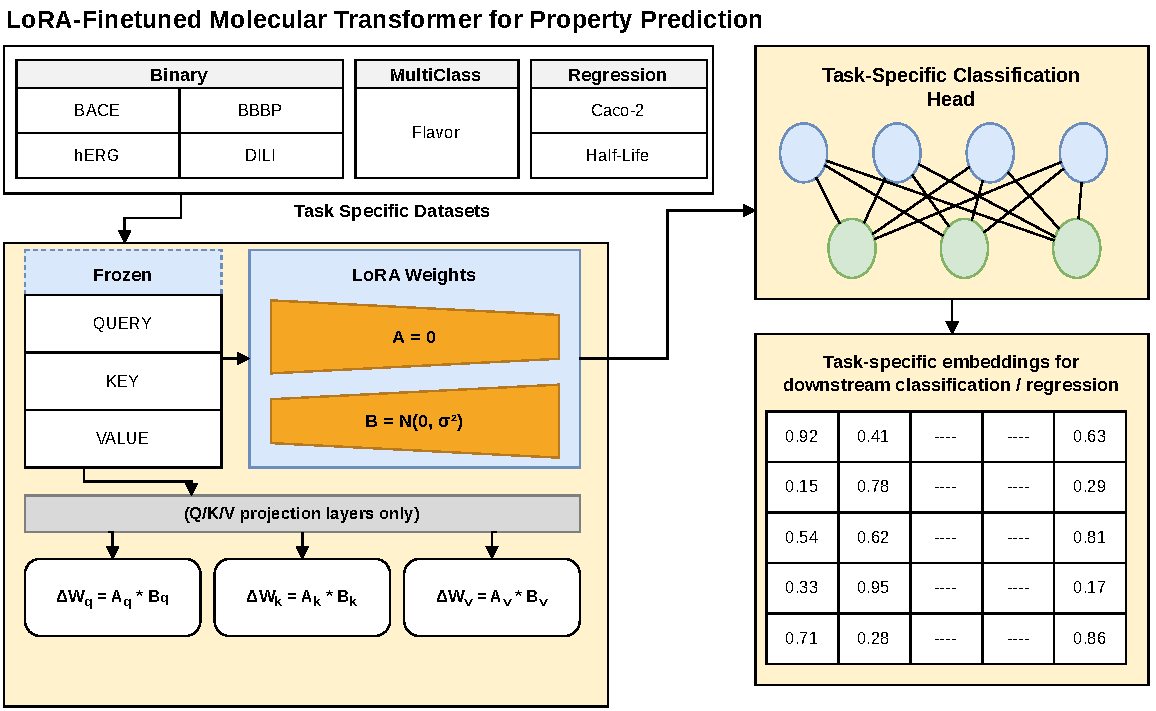
\includegraphics[width=0.99\textwidth]{ Figures_v2/LoRA_Finetuning_v2.pdf}
%DIFDELCMD <   %%%
\DIFdelendFL \DIFaddbeginFL \begin{subfigure}[t]{0.75\textwidth}
    \centering
    \includegraphics[width=\textwidth]{LoRA_FineTuning_v3.pdf}
    \DIFaddendFL \caption{\DIFdelbeginFL \DIFdelFL{Low-Rank Adaptation (LoRA) Architecture. A low-rank adaptation framework fine-tunes frozen transformer weights (Q/K/V layers) using trainable low-rank matrices (A, B), enabling efficient adaptation to task-specific molecular datasets including binary (hERG, DILI), multi-class (Flavor), and regression (Caco-2, Half-Life) targets.}\DIFdelendFL }
    \label{fig:lora-architecture}
  \DIFaddbeginFL \end{subfigure}
  \par\medskip
  \begin{subfigure}[t]{0.85\textwidth}
    \centering
    \includegraphics[width=\textwidth]{RAFE_Framework_v2.pdf}
    \caption{}
    \label{fig:rafe}
  \end{subfigure}
  \caption{\DIFaddFL{PEARL's two architectural components. }\textbf{\DIFaddFL{(a)}} \DIFaddFL{Low-Rank Adaptation (LoRA): a low-rank adaptation framework fine-tunes frozen transformer weights (Q/K/V layers) using trainable low-rank matrices (A, B), enabling efficient adaptation to task-specific molecular datasets including binary (hERG, DILI), multi-class (Flavor), and regression (Caco-2, Half-Life) targets. }\textbf{\DIFaddFL{(b)}} \DIFaddFL{Retrieval-Augmented Feature Enhancement (RAFE) pipeline: a query molecule is embedded by a task-specific finetuned CLM; the embedding retrieves $k$ nearest chemical neighbors from the ZINC-250k FAISS index (re-built independently per dataset). Four feature groups are extracted (physico-chemical neighborhood profile, density/isolation, embedding centroid, Tanimoto similarity), yielding a 60-dim RAFE vector concatenated with the CLM embedding and PC features for tree-based classification or regression.}}
  \label{fig:method_components}
\DIFaddendFL \end{figure}
Conformers for all dataset molecules are generated once before the hyperparameter sweep and cached, avoiding redundant ETKDGv3 calls during hyperparameter optimization. We use necessary flags to prevent conformer generation failures for metal-coordinated SMILES. Figure~\ref{fig:lora-architecture} illustrates how LoRA finetuning is implemented within our framework. All models use AdamW with cosine-annealing learning rate schedules; the encoder (LoRA adapters) receives the base learning rate while the classification/regression head receives $5\times$ the base rate. Gradient clipping ($\text{max\_norm} = 1.0$) is applied over all parameters, and early stopping monitors validation MCC (classification) or validation RMSE (regression) with patience of 5 epochs. Bayesian hyperparameter optimization with WandB sweeps ($20$-$30$ trials per dataset) optimizes for the corresponding validation metric.

\DIFaddbegin \FloatBarrier
\DIFaddend \subsection{Retrieval-Augmented Learning: the RAFE Component}\label{sec:rafe}

\subsubsection{Design Rationale and External Knowledge Base}\label{sec:zinc_rationale}
Naive retrieval-augmented approaches retrieve nearest neighbors from the task-specific training set and use their labels as auxiliary features. This introduces three problems: a small retrieval pool ($\sim$500-15,000 molecules depending on dataset), training-set leakage, and circular dependencies between the retrieval space and prediction target.

Unlike generative RAG~\cite{lewis2020rag}, where retrieved passages are injected into a language model prompt, RAFE does not pass retrieved content to any neural model. Retrieved ZINC-250k neighbors serve solely as a source of label-free physicochemical statistics (logP, QED, SAS distributions, structural similarity) that are featurized and concatenated with the molecular embedding before a tree-based model. The ``retrieval-augmented'' framing refers to the use of an external knowledge base at inference time, not to in-context generation.

PEARL addresses all three problems by using \textbf{ZINC-250k}~\cite{gomez2018automatic} as the retrieval corpus, i.e.\ a curated subset of $249,455$ drug-like molecules from the ZINC database~\cite{irwin2020zinc20} with no overlap with any training, validation, or test split, across all seven PEARL datasets. Each ZINC-250k molecule carries three physicochemical properties: lipophilicity (logP), Quantitative Estimate of Drug-likeness (QED $\in [0,1]$), and Synthetic Accessibility Score (SAS $\in [1,10]$).

ZINC-250k is chosen as the retrieval corpus for four complementary reasons:
\begin{enumerate}
  \item \textbf{Scale and diversity:} $249,455$ drug-like molecules span a broad region of chemical space, providing a dense and representative neighborhood for any query molecule from any of the seven PEARL datasets (the largest, hERG, has 13,445 compounds; the smallest, DILI, has 475).
  \item \textbf{Zero leakage:} ZINC-250k has no label overlap with any training, validation, or test split used in this study. Retrieved neighbors cannot carry prediction targets, eliminating the circular dependency that plagues training-set retrieval.
  \item \textbf{Label-free property signal:} logP, QED, and SAS are computed directly from SMILES without biological assay data. Their distributions in the local neighborhood of a query molecule characterize its physico-chemical environment in a way that is complementary to the molecule's own PC features and to the CLM's learned representation.
  \item \textbf{Model-family independence:} ZINC-250k is embedded independently by each finetuned CLM variant (ChemBERTa, MolFormer, Uni-Mol) and for each dataset, yielding model- and dataset-specific FAISS indices. RAFE features are therefore always expressed in the same geometric space as the query molecule's embedding.
\end{enumerate}

\subsubsection{Vector Indexing with FAISS}\label{sec:vector_faiss}
For each of the seven datasets, ZINC-250k molecules are re-embedded using that dataset's task-specific finetuned model variants. For binary/multi-class tasks, this means six SMILES-based variants (ChemBERTa-MLM $\times$ 2 loss, ChemBERTa-MTR $\times$ 2 loss, MolFormer $\times$ 2 loss) plus two Uni-Mol variants (FL and WL). For the two regression datasets, only a single Huber-loss variant is finetuned per CLM family, yielding three SMILES-based and one Uni-Mol variant.

SMILES-based embeddings are 768-dimensional CLS tokens; Uni-Mol embeddings are 2560-dimensional hybrid vectors (512-dim SE(3)-Transformer CLS concatenated with 2048-dim ECFP4 fingerprints). Embeddings are L2-normalized and indexed with FAISS \texttt{GpuIndexFlatIP}~\cite{johnson2021faiss}, a GPU-accelerated exact cosine-similarity search that achieves sub-2~ms query latency at 249k$\times$768 on a single GPU. The FAISS indices are serialized as CPU \texttt{IndexFlatIP} files for portable, fast retrieval.

\subsubsection{Chemical Neighborhood Feature Extraction}\label{sec:feature_extraction}
For every molecule in every split (train, validation, test), each FAISS index is queried by cosine similarity for the $k \in \{10, 20\}$ nearest ZINC-250k neighbors ($k$ fixed \DIFdelbegin \DIFdel{by design }\DIFdelend across all seven datasets\DIFaddbegin \DIFadd{; Section~\ref{sec:rafe_effectiveness} shows that the result does not depend on $k$}\DIFaddend ). Four feature groups are extracted:
\begin{itemize}
  \item[\textbf{(a)}] physico-chemical neighborhood profile (\DIFdelbegin \DIFdel{$\sim$27 }\DIFdelend \DIFaddbegin \DIFadd{18 }\DIFaddend features: mean/std of logP, QED, SAS at $k=10,20$, plus similarity-weighted means);
  \item[\textbf{(b)}] neighborhood density (5 features: nearest-neighbor similarity, mean/std of $k$-neighbor similarity at $k=10,20$);
  \item[\textbf{(c)}] embedding centroid features (\DIFdelbegin \DIFdel{$\sim$}\DIFdelend 34 features: PCA-32 compression of the $k=10$ neighbor centroid, fit on train only, plus similarity-to-centroid and centroid spread via standard deviation);
  \item[\textbf{(d)}] Tanimoto structural similarity (3 features: Morgan-fingerprint Tanimoto to the top-1 and top-5 neighbors, plus Murcko-scaffold overlap fraction in the top-10).
\end{itemize}
Together these four groups yield a \DIFdelbegin \DIFdel{69-dimensional }\DIFdelend \DIFaddbegin \DIFadd{60-dimensional }\DIFaddend RAFE feature vector \DIFaddbegin \DIFadd{(18 + 5 + 34 + 3) }\DIFaddend per molecule, concatenated as: [$\text{CLM embeddings} \mid \text{PC features (473-dim)} \mid \text{ZINC RAFE features}$] as depicted in Figure \ref{fig:rafe}.

\DIFdelbegin %DIFDELCMD < \begin{figure}[!ht]
%DIFDELCMD <   \centering
%DIFDELCMD <   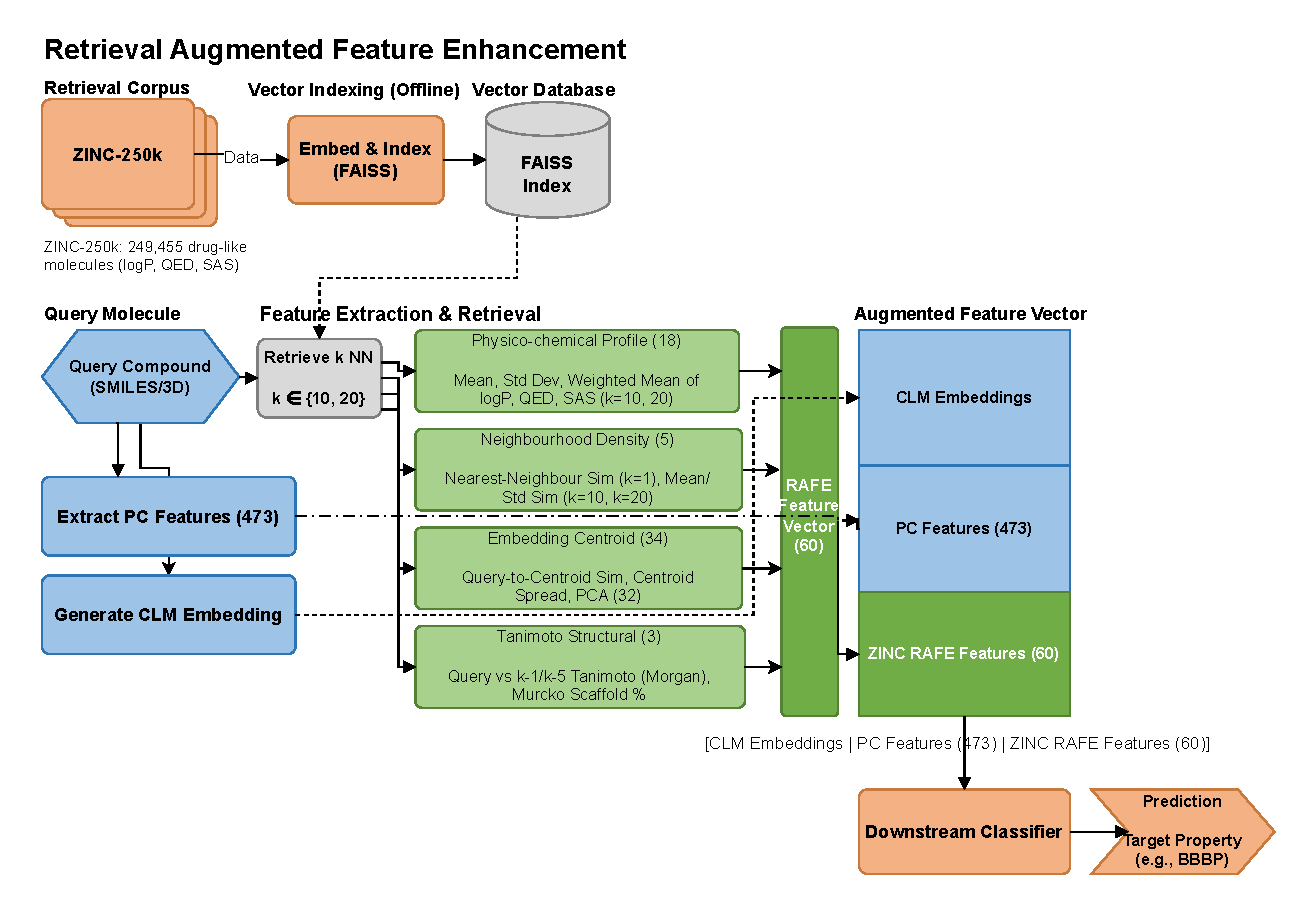
\includegraphics[width=0.99\textwidth]{ Figures_v2/RAFE_Framework_v2.pdf}
%DIFDELCMD <   %%%
%DIFDELCMD < \caption{%
{%DIFAUXCMD
\DIFdelFL{Retrieval-Augmented Feature Enhancement (RAFE) pipeline. A query molecule is embedded by a task-specific finetuned CLM; the embedding retrieves $k$ nearest chemical neighbors from the ZINC-250k FAISS index (re-built independently per dataset). Four feature groups are extracted (physico-chemical neighborhood profile, density/isolation, embedding centroid, Tanimoto similarity), yielding a 69-dim RAFE vector concatenated with the CLM embedding and PC features for tree-based classification or regression.}}
  %DIFAUXCMD
%DIFDELCMD < \label{fig:rafe}
%DIFDELCMD < \end{figure}
%DIFDELCMD < 

%DIFDELCMD < %%%
\DIFdelend \subsection{The PEARL Framework: Operational Ladder and Baselines}\label{sec:pearl_ladder}
Having introduced its three backbone CLMs, its LoRA adaptation mechanism, and its RAFE retrieval component, we can now describe how the PEARL framework assembles them. PEARL defines four operational modes that form a progressive evaluation ladder, applicable to both classification and regression targets:

\textbf{(a)~End-to-End (E2E) LoRA finetuning:} The CLM backbone (ChemBERTa, MolFormer, or Uni-Mol) with LoRA adapters and a task-specific head is optimized end-to-end for each downstream task. For binary tasks, the head is a dense layer with sigmoid activation; for multi-class tasks, a dense layer with softmax; for regression tasks (Caco-2, Half-Life), a single linear output unit trained with Huber loss.

\textbf{(b)~Finetuned Embedding Prediction (FT~Embed):} Task-specific embeddings are extracted from the finetuned model. For MolFormer, the CLS token passes through two dense layers with GELU activation (768-dim output). For ChemBERTa, the CLS token passes through a dense layer with tanh activation (384-dim). For Uni-Mol, the CLS token is concatenated with ECFP4 fingerprints (2560-dim). These embeddings train Optuna-tuned~\cite{akiba2019optuna} tree-based classifiers (XGBoost / LightGBM / CatBoost) or, for the two regression datasets, their regressor counterparts.

\textbf{(c)~FT~Embed $+$ PC (Physicochemical Feature Fusion):} The FT~Embed vector is concatenated with 473~domain-specific physicochemical (PC) features: 148 RDKit molecular descriptors, 30 graph-based features (NetworkX v3.5.2), 128-bit Morgan fingerprints, and 167-bit MACCS keys (RDKit v2025.09.4). This combined vector trains the same tree-based models without any retrieval from external databases. A full description of engineered features is provided in Supplementary Table~S1.

\textbf{(d)~Retrieval-Augmented Feature Enhancement (RAFE):} RAFE augments the FT~Embed $+$ PC feature vector with ZINC-250k chemical neighborhood features (\DIFdelbegin \DIFdel{69-dim}\DIFdelend \DIFaddbegin \DIFadd{60-dim}\DIFaddend ; Section~\ref{sec:rafe}), yielding the full feature vector [$\text{CLM embeddings} \mid \text{PC features (473-dim)} \mid \text{ZINC-250k RAFE features}$], passed to the same Optuna-tuned tree-based models.

\textbf{Baselines run in-house under the identical protocol, outside the ladder:} \textbf{PC-only} trains the same tree-model family directly on the 473-dim PC vector, with \emph{no} CLM component, isolating how much of the ladder's performance is attributable to the CLM. \textbf{Chemprop}~\cite{yang2019chemprop} (D-MPNN) and a \textbf{GCN} (GINConv-based, hand-rolled, atom/bond-featurized) are both trained end-to-end on the molecular graph, on the same scaffold split, with the same Optuna-style hyperparameter search budget and the same bootstrapped-CI evaluation as every CLM-based method above.

\subsection{Loss Functions for Class Imbalance and Regression}\label{sec:loss_functions}
Three loss functions address class imbalance (classification) or robust regression, implemented via a custom extension of the HuggingFace \texttt{Trainer}.

\noindent \textbf{Weighted cross-entropy (WL):} $\mathcal{L}_{\text{WL}} = -\sum_{i=0}^{C-1} w_i y_i \log\hat{y}_i$, where $w_i = 1 - f_i$ (inverse class frequency). This gives the minority class higher loss contribution and is most effective for datasets like BACE and Flavor.

\noindent\textbf{Focal loss (FL):} \DIFdelbegin \DIFdel{$\mathcal{L}_{\text{FL}} = -\alpha (1 - \hat{p}_i)^\gamma \log\hat{p}_i$ }\DIFdelend \DIFaddbegin \DIFadd{$\mathcal{L}_{\text{FL}} = -\alpha_c (1 - \hat{p}_c)^\gamma \log\hat{p}_c$ for the true class $c$, }\DIFaddend with $\gamma = 2$ \DIFaddbegin \DIFadd{and per-class weights $\alpha_c = 1 - f_c$ (one minus the training-set class frequency)}\DIFaddend , which down-weights well-classified examples to focus learning on hard-to-classify boundary cases. This excels on heavily imbalanced and challenging classification tasks. hERG and DILI both use FL and WL sweeps, matching the same protocol used for BACE, BBBP, and Flavor.

\noindent\textbf{Huber loss (regression):} $\mathcal{L}_{\text{Huber}}(y, \hat y) = \begin{cases}\tfrac{1}{2}(y-\hat y)^2 & |y - \hat y| \le \delta \\ \delta(|y-\hat y| - \tfrac12 \delta) & \text{otherwise}\end{cases}$, with $\delta = 1.0$. Huber loss is used for both \DIFdelbegin \DIFdel{Caco-2 and Half-Life regression targets, combining }\DIFdelend \DIFaddbegin \DIFadd{regression targets. It combines }\DIFaddend MSE's smoothness near zero error with MAE's robustness to the outlier-prone tail of half-life measurements (\DIFaddbegin \DIFadd{the }\DIFaddend Half-Life \DIFdelbegin \DIFdel{'s target is additionally }\DIFdelend \DIFaddbegin \DIFadd{target is also }\DIFaddend log1p-transformed before \DIFaddbegin \DIFadd{the }\DIFaddend Huber loss is applied, and predictions are inverse-transformed before evaluation).

\subsection{Tree-Based Prediction Models}\label{sec:tree_models}
The final prediction stage employs XGBoost~\cite{chen2016xgboost}, LightGBM~\cite{ke2017lightgbm}, and CatBoost~\cite{prokhorenkova2018catboost}, in their classifier or regressor form as appropriate. These algorithms handle high-dimensional mixed-type feature vectors, provide built-in feature importance, and are robust to outliers. \DIFdelbegin \DIFdel{Bayesian hyperparameter optimization was performed }\DIFdelend \DIFaddbegin \DIFadd{Hyperparameters were tuned }\DIFaddend with Optuna~\cite{akiba2019optuna} ($20$ trials for each configuration) \DIFdelbegin \DIFdel{maximizing validation }\DIFdelend \DIFaddbegin \DIFadd{on the training split only, maximizing }\DIFaddend MCC (classification, \DIFdelbegin \DIFdel{via }\DIFdelend stratified 5-fold \DIFdelbegin \DIFdel{CV}\DIFdelend \DIFaddbegin \DIFadd{cross-validation}\DIFaddend ) or minimizing \DIFdelbegin \DIFdel{validation }\DIFdelend RMSE (regression, \DIFdelbegin \DIFdel{via }\DIFdelend 5-fold \DIFdelbegin \DIFdel{CV}\DIFdelend \DIFaddbegin \DIFadd{cross-validation}\DIFaddend ). Class-weighting strategies address imbalance for classification tasks (\texttt{scale\_pos\_weight}, \texttt{class\_weight="balanced"}, \texttt{auto\_class\_weights="Balanced"} for XGBoost/LightGBM/CatBoost respectively); regression targets are otherwise unweighted.

%% =====================================================================
\section{Experimental Setup and Benchmarking}\label{sec:experimental_setup}
The seven datasets, their splits, and class/label distributions used throughout this benchmark are described in Section~\ref{sec:datasets} (Table~\ref{tab:dataset_summary}).

\subsection{Baseline Models}\label{sec:baselines}
PEARL's four operational modes are compared against three in-house baselines run under the identical scaffold split, preprocessing, and evaluation protocol: \textbf{PC-only} (no CLM, no LoRA, no retrieval), \textbf{Chemprop}~\cite{yang2019chemprop} (D-MPNN), and a hand-rolled \textbf{GCN} (GINConv-based). \DIFdelbegin \DIFdel{Additionally, on the }\DIFdelend \DIFaddbegin \DIFadd{We also train the same tree models on conventional fingerprints and descriptors (ECFP4, ECFP6, MACCS, ECFP4$+$MACCS and the RDKit descriptor set), under the same splits and tuning. On the }\DIFaddend three MoleculeNet-era datasets (BACE, BBBP, Flavor)\DIFdelbegin \DIFdel{where comparable external LoRA/GNN }\DIFdelend \DIFaddbegin \DIFadd{, for which comparable }\DIFaddend literature numbers exist, PEARL is compared against published external baselines: Chemprop~\cite{yang2019chemprop}, GROVER~\cite{rong2020grover}, AttentiveFP~\cite{xiong2020attentivefp}, Mole-BERT~\cite{xia2023molecbert}, and the original Uni-Mol and MolFormer full-finetuning results (Section~\ref{sec:external_comparison}). The four TDC ADMET Group tasks have no comparable external LoRA/RAFE literature baseline, so their comparison is entirely in-house.

\subsection{Evaluation Protocol\DIFaddbegin \DIFadd{, Model Selection }\DIFaddend and \DIFdelbegin \DIFdel{Implementation Details}\DIFdelend \DIFaddbegin \DIFadd{Statistics}\DIFaddend }\label{sec:eval_protocol}
\DIFdelbegin \DIFdel{For classification, performance is evaluated using accuracy(Acc)}\DIFdelend \DIFaddbegin \paragraph{\DIFadd{Metrics.}} \DIFadd{For classification we report accuracy}\DIFaddend , area under the ROC curve (AUC), Matthews correlation coefficient (MCC), precision\DIFdelbegin \DIFdel{(Prec), recall (Rec), and F1-macro (}\DIFdelend \DIFaddbegin \DIFadd{, recall and }\DIFaddend F1 \DIFdelbegin \DIFdel{$_\text{mac}$}\DIFdelend \DIFaddbegin \DIFadd{(macro and micro}\DIFaddend )\DIFdelbegin \DIFdel{/ F1-micro (F1$_\text{mic}$)}\DIFdelend ; MCC is the primary ranking metric \DIFdelbegin \DIFdel{due to its robustness to class imbalance }\DIFdelend \DIFaddbegin \DIFadd{because it is robust to class imbalance \mbox{%DIFAUXCMD
\cite{mall2024vishpred,mall2013furs,mall2014representative}}\hskip0pt%DIFAUXCMD
}\DIFaddend . For the two regression datasets (Caco-2, Half-Life) \DIFdelbegin \DIFdel{, }\DIFdelend we report R\textsuperscript{2}, mean absolute error \DIFdelbegin \DIFdel{(MAE), }\DIFdelend and Spearman rank correlation\DIFaddbegin \DIFadd{, and rank by Spearman}\DIFaddend .

\DIFdelbegin \DIFdel{Most datasets in this study have small-to-moderate test sets (DILI $n=96$; BACE $n\approx152$; Caco-2 $n=182$; Half-Life $n=133$), so }\textbf{\DIFdel{performance differences are interpreted alongside bootstrapped confidence intervals}} %DIFAUXCMD
\DIFdel{(10}\DIFdelend \DIFaddbegin \paragraph{\DIFadd{Tuning and model selection.}} \DIFadd{All tree models are tuned on the training split only: 20 Optuna trials per configuration, 5-fold cross-validation, and balanced sample weights for classification. The test split is evaluated once per fitted model and is never used for tuning. LoRA fine-tuning uses the fixed training and validation splits (the validation split for monitoring and early stopping), not cross-validation. Configurations (embedding model, loss, tree model and stage) are compared on the test set, as is usual for benchmarks. Because the best configuration is selected on the same test set, its score is optimistic. We therefore report five-seed means next to every single-run best value, and the paired difference between the best and the runner-up configuration (Table~\ref{tab:best_configs}).
}

\paragraph{\DIFadd{Seeds and paired statistics.}} \DIFadd{Every downstream arm is run with five seeds (42 to 46). The seed sets the Optuna sampler, the cross-validation shuffle and the model initialization. Two arms are compared with a paired bootstrap on identical test molecules: in each of 3}\DIFaddend {,}000 resamples \DIFaddbegin \DIFadd{the test molecules are resampled once, the metric difference is computed for each seed and averaged over seeds, and the 2.5th and 97.5th percentiles give a 95\% interval. We call a difference significant when this interval excludes zero. The 10}{\DIFaddend ,\DIFdelbegin \DIFdel{stratified by class label for classification, unstratified for regression with normal-approximation, computed on the fixed test-set predictions without retraining). We use a }\textbf{\DIFdel{$\pm 1$ SE}} %DIFAUXCMD
\DIFdel{band for statistical difference during head-to-head comparisons. }\DIFdelend \DIFaddbegin }\DIFadd{000-resample standard errors in the single-run tables and in Figure~\ref{fig:results_summary} are descriptive. Comparisons between configurations that share a test set (for example Wilcoxon tests over matched configurations) are likewise descriptive.
}\DIFaddend 

\DIFaddbegin \paragraph{\DIFadd{Scope of the variability estimates.}} \DIFadd{The seeds cover the downstream tree stage. LoRA fine-tuning, the re-embedding of ZINC-250k and the end-to-end LoRA, Chemprop and GCN baselines are single runs, so the intervals are lower bounds on the total variability. The new experiments ran XGBoost on GPU, so absolute values differ slightly from the original CPU runs; arms are therefore always compared within one experiment.
}

\paragraph{\DIFadd{Implementation.}} \DIFaddend All training uses AdamW with cosine-annealing learning rate schedules\DIFdelbegin \DIFdel{and Bayesian hyperparameter optimization via }\DIFdelend \DIFaddbegin \DIFadd{. LoRA hyperparameters were searched with }\DIFaddend WandB sweeps ($20$-$30$ trials per dataset\DIFdelbegin \DIFdel{for LoRA finetuning)or Optuna~\mbox{%DIFAUXCMD
\cite{akiba2019optuna} }\hskip0pt%DIFAUXCMD
($20$ trials per configuration for the tree-based stage). Exact per-run hardware configuration}\DIFdelend \DIFaddbegin \DIFadd{). Hardware}\DIFaddend , environment specification \DIFdelbegin \DIFdel{, }\DIFdelend and wall-clock timings are documented in the \DIFdelbegin \DIFdel{accompanying }\DIFdelend code repository (\url{https://github.com/raghvendra5688/PEARL})\DIFdelbegin \DIFdel{to support full reproducibility}\DIFdelend .

%% =====================================================================
\section{Results and Discussion}\label{sec:results_discussion}

We \DIFdelbegin \DIFdel{oragnize }\DIFdelend \DIFaddbegin \DIFadd{organize }\DIFaddend the results around the four PEARL operational modes described in Section~\ref{sec:pearl_ladder}, plus the \DIFdelbegin \DIFdel{three }\DIFdelend in-house baselines (PC-only, Chemprop, GCN) run identically across all seven datasets: (i)~\textbf{E2E LoRA}\DIFdelbegin \DIFdel{: }\DIFdelend \DIFaddbegin \DIFadd{, }\DIFaddend end-to-end LoRA finetuning of the CLM backbone; (ii)~\textbf{FT Embed}\DIFdelbegin \DIFdel{: }\DIFdelend \DIFaddbegin \DIFadd{, }\DIFaddend Optuna-tuned tree models on frozen finetuned embeddings; (iii)~\textbf{FT Embed $+$ PC}\DIFdelbegin \DIFdel{: }\DIFdelend \DIFaddbegin \DIFadd{, }\DIFaddend FT Embed augmented with \DIFdelbegin \DIFdel{473-dim physicochemical features, without ZINC-250k retrieval; }\DIFdelend \DIFaddbegin \DIFadd{473 physicochemical features; and }\DIFaddend (iv)~\textbf{RAFE}\DIFdelbegin \DIFdel{: }\DIFdelend \DIFaddbegin \DIFadd{, }\DIFaddend FT Embed $+$ PC \DIFdelbegin \DIFdel{further }\DIFdelend augmented with ZINC-250k neighborhood features. \DIFdelbegin \DIFdel{For each mode , we report the best-performing CLM variant and , where applicable, the corresponding tree model. Full ablation tables for each dataset are provided in the Supplementary Material}\DIFdelend \DIFaddbegin \DIFadd{The per-dataset tables (Section~\ref{sec:main_results}) give the best configuration of each mode from single runs. Sections~\ref{sec:controlled} to~\ref{sec:fingerprints} then repeat the comparison under controlled conditions and on five-seed means, and Sections~\ref{sec:rafe_effectiveness} to~\ref{sec:efficiency} examine H2, H3 and H1 in turn}\DIFaddend .

\subsection{Main Benchmarking Results}\label{sec:main_results}

\subsubsection{Sequence of Comparisons}\label{sec:comparison_sequence}
The four PEARL modes form \DIFdelbegin \DIFdel{an evaluation }\DIFdelend \DIFaddbegin \DIFadd{a }\DIFaddend ladder that isolates the contribution of each component\DIFdelbegin \DIFdel{, bracketed on one end by }\DIFdelend \DIFaddbegin \DIFadd{. }\DIFaddend \textbf{PC-only} (no CLM\DIFdelbegin \DIFdel{at all) and on the other by }\textbf{\DIFdel{E2E LoRA}} %DIFAUXCMD
\DIFdel{(fully differentiable gradient flow): }\textbf{\DIFdel{PC-only}} %DIFAUXCMD
\DIFdel{establishes the floorachievable with no CLM - any }\DIFdelend \DIFaddbegin \DIFadd{) sets the floor: a }\DIFaddend CLM-based method that \DIFdelbegin \DIFdel{fails to }\DIFdelend \DIFaddbegin \DIFadd{does not }\DIFaddend beat it has not \DIFdelbegin \DIFdel{demonstrated }\DIFdelend \DIFaddbegin \DIFadd{shown }\DIFaddend that its added \DIFdelbegin \DIFdel{architectural and computational complexity is earning its keep }\DIFdelend \DIFaddbegin \DIFadd{complexity pays off }\DIFaddend on that dataset. \textbf{E2E LoRA} \DIFdelbegin \DIFdel{establishes the ceiling achievable by fully differentiable }\DIFdelend \DIFaddbegin \DIFadd{is the reference for end-to-end }\DIFaddend gradient flow through the \DIFdelbegin \DIFdel{CLM backbone, treated as the upper bound for each CLM family and dataset}\DIFdelend \DIFaddbegin \DIFadd{backbone}\DIFaddend . \textbf{FT Embed} \DIFdelbegin \DIFdel{quantifies how much embedding quality alone contributes ; any gap between FT Embed and }\DIFdelend \DIFaddbegin \DIFadd{measures what the embedding contributes alone, and any gap to }\DIFaddend E2E LoRA reflects information recoverable only through end-to-end \DIFdelbegin \DIFdel{gradient flow}\DIFdelend \DIFaddbegin \DIFadd{training}\DIFaddend . \textbf{FT Embed $+$ PC} isolates the \DIFdelbegin \DIFdel{contribution of physicochemical feature engineering}\DIFdelend \DIFaddbegin \DIFadd{physicochemical features}\DIFaddend , independent of \DIFdelbegin \DIFdel{any external }\DIFdelend retrieval. \textbf{RAFE} measures the \DIFdelbegin \DIFdel{additional }\DIFdelend \DIFaddbegin \DIFadd{added }\DIFaddend value of ZINC-250k \DIFdelbegin \DIFdel{chemical }\DIFdelend neighborhood context: a gain \DIFdelbegin \DIFdel{from }\DIFdelend \DIFaddbegin \DIFadd{over }\DIFaddend FT Embed $+$ PC \DIFdelbegin \DIFdel{to RAFE suggests that neighborhood signals from ZINC-250k provide information orthogonal to }\DIFdelend \DIFaddbegin \DIFadd{would suggest information beyond }\DIFaddend both the learned \DIFdelbegin \DIFdel{CLM }\DIFdelend representation and the molecule's own physicochemical profile. \textbf{Chemprop and GCN}, run in-house on the identical split and protocol, \DIFdelbegin \DIFdel{provide }\DIFdelend \DIFaddbegin \DIFadd{are }\DIFaddend graph-based \DIFdelbegin \DIFdel{reference points that isolate the contribution of }\DIFdelend \DIFaddbegin \DIFadd{references that isolate }\DIFaddend explicit bond-graph message passing, independent of any CLM pretraining corpus.

\DIFdelbegin \DIFdel{By applying a $\pm 1$~SE overlap test between each dataset's point-estimate winner and PC-only, }\textbf{\DIFdel{none of the four TDC ADMET datasets (hERG, DILI, Caco-2, Half-Life) shows a statistically confirmed win over PC-only}}%DIFAUXCMD
\DIFdel{: every point-estimate winner's $\pm 1$~SE band overlaps PC-only's. This mirrors the pattern already observed for Flavor. }\DIFdelend \DIFaddbegin \DIFadd{The per-dataset tables below report single-run best configurations. Their standard errors are descriptive, because the best row of each mode is chosen on the test set. Formal comparisons use paired bootstrap intervals on identical test molecules (Section~\ref{sec:eval_protocol}) and are reported in Section~\ref{sec:controlled}. }\DIFaddend Figure~\ref{fig:results_summary} \DIFdelbegin \DIFdel{summarizes the mean$\pm$SE primary metric for every method across }\DIFdelend \DIFaddbegin \DIFadd{shows the single-run primary metric of every method on }\DIFaddend all seven datasets.

\begin{figure*}[!ht]
  \centering
  \DIFdelbeginFL %DIFDELCMD < 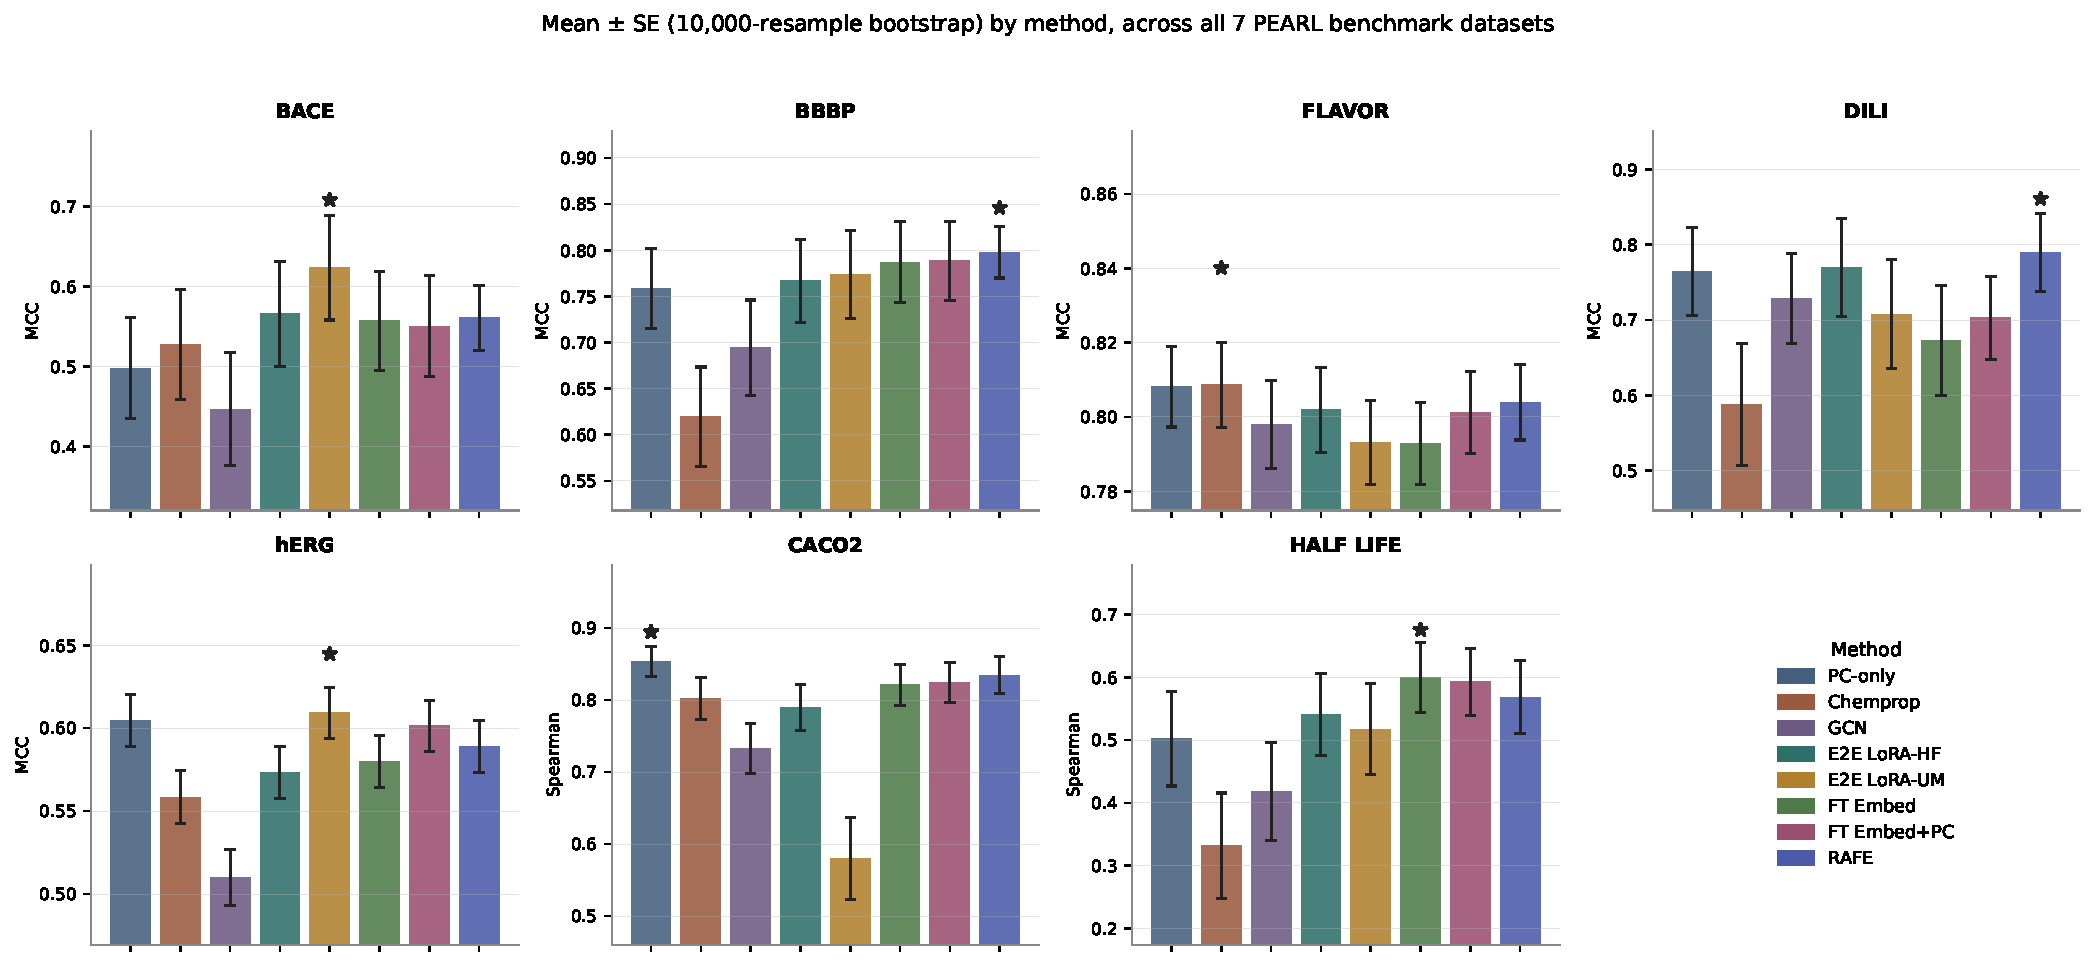
\includegraphics[width=0.99\textwidth]{ Figures_v2/results_summary_v2.pdf}
%DIFDELCMD <   %%%
\DIFdelendFL \DIFaddbeginFL \includegraphics[width=0.99\textwidth]{results_summary_v2.pdf}
  \DIFaddendFL \caption{Mean $\pm$ SE (10,000-resample bootstrap) of the primary ranking metric (MCC for classification, Spearman for regression) for every method across all seven PEARL benchmark datasets. Stars mark the point-estimate winner per dataset. \DIFdelbeginFL \DIFdelFL{Whisker overlap between }\DIFdelendFL \DIFaddbeginFL \DIFaddFL{Values are single runs of }\DIFaddendFL the \DIFdelbeginFL \DIFdelFL{winner and PC-only means the win is not statistically confirmed at $\pm1$~SE}\DIFdelendFL \DIFaddbeginFL \DIFaddFL{best configuration of each method}\DIFaddendFL ; \DIFdelbeginFL \DIFdelFL{this is }\DIFdelendFL the \DIFdelbeginFL \DIFdelFL{case for six }\DIFdelendFL \DIFaddbeginFL \DIFaddFL{bars are descriptive and not a test }\DIFaddendFL of \DIFdelbeginFL \DIFdelFL{seven datasets (all but BACE)}\DIFdelendFL \DIFaddbeginFL \DIFaddFL{the difference}\DIFaddendFL .}
  \label{fig:results_summary}
\end{figure*}

\DIFaddbegin \FloatBarrier
\DIFaddend \subsubsection{BBBP Dataset Results}
\DIFdelbegin \DIFdel{Table~\ref{tab:bbbp} presents the }\DIFdelend \DIFaddbegin \DIFadd{The }\DIFaddend best configuration per modality and CLM family for BBBP \DIFdelbegin \DIFdel{. }\textbf{\DIFdel{RAFE with MolFormer-XL (FL~+~XGBoost) achieves the best overall result}} %DIFAUXCMD
\DIFdel{(}\DIFdelend \DIFaddbegin \DIFadd{(single runs; Supplementary Table~S2) is RAFE with MolFormer-XL (FL~$+$~XGBoost; }\DIFaddend MCC$=0.798$, AUC$=0.940$, SE$=0.028$), \DIFdelbegin \DIFdel{$\approx 4\%$ }\DIFdelend ahead of E2E LoRA MolFormer FL (MCC$=0.767$, AUC$=0.929$) and Uni-Mol E2E LoRA WL (MCC$=0.774$, AUC$=0.943$)\DIFdelbegin \DIFdel{w. r. t. MCCmetric. RAFE's gain over }\DIFdelend \DIFaddbegin \DIFadd{. This single-run value is optimistic. The same configuration averages MCC$=\mBBBPRAFE \pm \sBBBPRAFE$ over five seeds, and }\DIFaddend FT Embed+PC \DIFdelbegin \DIFdel{(MolFormer-XL FL + LightGBM, MCC$=0.789$) and over Uni-Mol RAFE (FL + XGBoost, MCC$=0.773$)points to ZINC-250k neighborhood context - high mean logP of retrieved neighbors, associated with BBB-permeable molecules - as an interpretable, complementary signal}\DIFdelend \DIFaddbegin \DIFadd{with the same embedding and tree averages $\mBBBPFTPC \pm \sBBBPFTPC$ (single run: $\srBBBPFTPC$). Within the same tree, the two stages are indistinguishable (Supplementary Table~S10)}\DIFaddend . PC-only \DIFdelbegin \DIFdel{is a strong baseline here too (}\DIFdelend \DIFaddbegin \DIFadd{reaches }\DIFaddend MCC$=0.759$ \DIFdelbegin \DIFdel{, AUC$=0.937$): RAFE 's point-estimate gain over it is $+0.039$ MCC, and their $\pm1$~SE bands ($0.798\pm0.028$ vs.\ $0.759\pm0.043$)are close to non-overlapping, the strongest of the two confirmed-adjacent ``wins'' reported in this paper}\DIFdelend \DIFaddbegin \DIFadd{in the original table and $\mBBBPPC$ over five seeds (best tree). The advantage of RAFE over the fine-tuned embedding alone is small ($+0.014$ on average over matched configurations, Wilcoxon $p=0.025$; Figure~\ref{fig:ladder}). In the controlled matrix, FT Embed+PC is $+0.054$ above PC-only with XGBoost (95\% interval $-0.017$ to $+0.130$), so we read BBBP as a dataset where fine-tuned embeddings tend to help over descriptors and RAFE adds no measurable benefit beyond them}\DIFaddend . Full per-embedding, per-loss \DIFdelbegin \DIFdel{ablation is }\DIFdelend \DIFaddbegin \DIFadd{results are }\DIFaddend in Supplementary Table~S2.

\DIFdelbegin %DIFDELCMD < \begin{table*}[!ht]
%DIFDELCMD < \centering
%DIFDELCMD < %%%
%DIFDELCMD < \caption{%
{%DIFAUXCMD
\DIFdelFL{Best performing configurations for each modality/baseline on BBBP. $^*$ denotes overall best by MCC. RAFE = FT~Embed~+~PC~+~ZINC-250k retrieval features. PC-only / Chemprop / GCN are run in-house on the identical split.}}
%DIFAUXCMD
%DIFDELCMD < \label{tab:bbbp}
%DIFDELCMD < \resizebox{0.95\textwidth}{!}{
%DIFDELCMD < \begin{tabular}{lllllrrrrrrr}
%DIFDELCMD < \toprule
%DIFDELCMD < Modality & CLM & Loss & ML & AUC & Acc & F1$_\text{mac}$ & F1$_\text{mic}$ & MCC & Prec & Rec & SE(MCC) \\
%DIFDELCMD < \midrule
%DIFDELCMD < PC-only    & --- & --- & LightGBM & 0.937 & 0.885 & 0.867 & 0.885 & 0.759 & 0.916 & 0.846 & 0.043 \\
%DIFDELCMD < Chemprop   & --- & --- & --- & 0.918 & 0.807 & 0.801 & 0.807 & 0.620 & 0.799 & 0.821 & 0.054 \\
%DIFDELCMD < GCN        & --- & --- & --- & 0.924 & 0.859 & 0.839 & 0.859 & 0.694 & 0.874 & 0.822 & 0.052 \\
%DIFDELCMD < \midrule
%DIFDELCMD < E2E LoRA   & MolFormer-XL & FL & --- & 0.929 & 0.891 & 0.874 & 0.891 & 0.767 & 0.913 & 0.856 & 0.045 \\
%DIFDELCMD < E2E LoRA   & Uni-Mol      & WL & --- & 0.943 & 0.896 & 0.887 & 0.896 & 0.774 & 0.890 & \textbf{0.885} & 0.048 \\
%DIFDELCMD < \midrule
%DIFDELCMD < FT Embed   & MolFormer-XL & FL & XGBoost & 0.935 & 0.901 & 0.888 & 0.901 & 0.787 & 0.914 & 0.873 & 0.044 \\
%DIFDELCMD < FT Embed+PC& MolFormer-XL & FL & LightGBM& 0.934 & 0.901 & 0.887 & 0.901 & 0.789 & 0.920 & 0.870 & 0.043 \\
%DIFDELCMD < \midrule
%DIFDELCMD < RAFE$^*$   & MolFormer-XL & FL & XGBoost & \textbf{0.940} & \textbf{0.906} & \textbf{0.895} & \textbf{0.906} & \textbf{0.798} & \textbf{0.918} & 0.881 & \textbf{0.028} \\
%DIFDELCMD < RAFE       & Uni-Mol      & FL & XGBoost & 0.928 & 0.891 & 0.872 & 0.891 & 0.773 & 0.927 & 0.850 & --- \\
%DIFDELCMD < \bottomrule
%DIFDELCMD < \end{tabular}
%DIFDELCMD < }
%DIFDELCMD < \end{table*}
%DIFDELCMD < 

%DIFDELCMD < %%%
\DIFdelend \DIFaddbegin \FloatBarrier
\DIFaddend \subsubsection{Flavor Dataset Results}
\DIFdelbegin \DIFdel{Table~\ref{tab:flavor} }\DIFdelend \DIFaddbegin \DIFadd{Supplementary Table~S3 }\DIFaddend presents results on the multi-class Flavor dataset \DIFdelbegin \DIFdel{. }\textbf{\DIFdel{RAFE (MolFormer-XL WL + CatBoost) achieves MCC$=0.804$}} %DIFAUXCMD
\DIFdel{(}\DIFdelend \DIFaddbegin \DIFadd{(single runs). RAFE (MolFormer-XL WL~$+$~CatBoost) reaches MCC$=0.804$ (}\DIFaddend AUC$=0.963$, Prec$=0.868$, Rec$=0.749$, SE$=0.010$), \DIFdelbegin \DIFdel{statistically indistinguishable from }\DIFdelend \DIFaddbegin \DIFadd{within one standard error of }\DIFaddend Chemprop (MCC$=0.809$, SE\DIFdelbegin \DIFdel{$=0.0115$}\DIFdelend \DIFaddbegin \DIFadd{$=0.011$}\DIFaddend ) and PC-only (MCC$=0.808$, SE\DIFdelbegin \DIFdel{$=0.0108$)at $\pm1$~SE -- all four bands overlap heavily on this }\DIFdelend \DIFaddbegin \DIFadd{$=0.011$). The test set is }\DIFaddend large ($n_\text{test}=2{,}254$), \DIFdelbegin \DIFdel{well-powered test set. This is a dataset where the CLM ladder }\DIFdelend \DIFaddbegin \DIFadd{so the controlled comparison is informative: with XGBoost, RAFE is significantly below PC-only ($-0.027$, 95\% interval $-0.044$ to $-0.010$; Table~\ref{tab:controlled}), and with LightGBM and CatBoost the intervals include zero. The CLM ladder therefore }\DIFaddend does not clear the PC-only \DIFdelbegin \DIFdel{/ GNN baselines by any meaningful margin}\DIFdelend \DIFaddbegin \DIFadd{and GNN baselines on this dataset}\DIFaddend . Uni-Mol reaches MCC$=0.795$ with weighted loss, competitive with but below MolFormer, \DIFdelbegin \DIFdel{a sign }\DIFdelend \DIFaddbegin \DIFadd{which suggests }\DIFaddend that 3D geometry \DIFdelbegin \DIFdel{does not add much }\DIFdelend \DIFaddbegin \DIFadd{adds little }\DIFaddend for taste prediction. \DIFaddbegin \DIFadd{Over five seeds and the full grid the three stages are close together (FT Embed }\mFLAVFT{}\DIFadd{, FT Embed+PC }\mFLAVFTPC{}\DIFadd{, RAFE }\mFLAVRAFE{}\DIFadd{) and all sit just below the descriptor baseline (}\mFLAVPC{}\DIFadd{). }\DIFaddend The full per-embedding, per-loss ablation is in Supplementary Table~S3.

\DIFdelbegin %DIFDELCMD < \begin{table*}[t]
%DIFDELCMD < \centering
%DIFDELCMD < %%%
%DIFDELCMD < \caption{%
{%DIFAUXCMD
\DIFdelFL{Best performing configurations on Flavor. Prec/Rec are macro-averaged; AUC is one-vs-rest macro ROC AUC.}}
%DIFAUXCMD
%DIFDELCMD < \label{tab:flavor}
%DIFDELCMD < \resizebox{0.95\textwidth}{!}{
%DIFDELCMD < \begin{tabular}{lllllrrrrrrr}
%DIFDELCMD < \toprule
%DIFDELCMD < Modality & CLM & Loss & ML & AUC & Acc & F1$_\text{mac}$ & F1$_\text{mic}$ & MCC & Prec & Rec & SE(MCC) \\
%DIFDELCMD < \midrule
%DIFDELCMD < PC-only    & --- & --- & XGBoost  & 0.972 & 0.890 & 0.761 & 0.890 & 0.808 & 0.733 & 0.798 & 0.0108 \\
%DIFDELCMD < Chemprop   & --- & --- & --- & 0.974 & \textbf{0.899} & \textbf{0.809} & \textbf{0.899} & \textbf{0.809} & 0.796 & 0.835 & 0.0115 \\
%DIFDELCMD < GCN        & --- & --- & --- & 0.973 & 0.893 & 0.814 & 0.893 & 0.798 & 0.834 & 0.800 & 0.0118 \\
%DIFDELCMD < \midrule
%DIFDELCMD < E2E LoRA   & MolFormer-XL & WL & --- & \textbf{0.975} & 0.892 & \textbf{0.809} & 0.892 & 0.802 & 0.802 & 0.817 & 0.0115 \\
%DIFDELCMD < \midrule
%DIFDELCMD < FT Embed   & MolFormer-XL & WL & LightGBM& 0.970 & 0.882 & 0.783 & 0.882 & 0.787 & 0.800 & 0.778 & 0.0111 \\
%DIFDELCMD < FT Embed+PC& MolFormer-XL & WL & CatBoost& 0.958 & 0.888 & 0.772 & 0.888 & 0.801 & 0.756 & 0.793 & 0.0111 \\
%DIFDELCMD < \midrule
%DIFDELCMD < RAFE       & MolFormer-XL & WL & CatBoost& 0.963 & 0.893 & 0.774 & 0.893 & 0.804 & \textbf{0.868} & 0.749 & 0.0102 \\
%DIFDELCMD < \bottomrule
%DIFDELCMD < \end{tabular}
%DIFDELCMD < }
%DIFDELCMD < \end{table*}
%DIFDELCMD < 

%DIFDELCMD < %%%
\DIFdelend \DIFaddbegin \FloatBarrier
\DIFaddend \subsubsection{BACE Dataset Results}
\DIFdelbegin \DIFdel{Table~\ref{tab:bace} }\DIFdelend \DIFaddbegin \DIFadd{Supplementary Table~S4 }\DIFaddend compares key configurations on BACE. BACE remains the most challenging dataset here (MCC $< 0.65$ across all methods). \DIFdelbegin \DIFdel{Figure~\ref{fig:bace} }\DIFdelend \DIFaddbegin \DIFadd{Supplementary Figure~S1 }\DIFaddend compares the AUC and AUPR of Uni-Mol E2E LoRA with counterparts in the CLM ladder\DIFdelbegin \DIFdel{. }\DIFdelend \DIFaddbegin \DIFadd{, where Uni-Mol WL attains the highest AUPR of the configurations shown. }\DIFaddend \textbf{Uni-Mol with weighted loss \DIFdelbegin \DIFdel{achieves }\DIFdelend \DIFaddbegin \DIFadd{gives }\DIFaddend the \DIFdelbegin \DIFdel{best overall performance}\DIFdelend \DIFaddbegin \DIFadd{highest single-run value}\DIFaddend } (MCC$=0.623$, SE$=0.039$; AUC$=0.891$; Acc$=0.822$), \DIFdelbegin \DIFdel{an 8\% absolute MCC gain over }\DIFdelend \DIFaddbegin \DIFadd{$0.057$ above }\DIFaddend the next-best SMILES-based E2E LoRA (MolFormer-XL FL, MCC$=0.566$, SE$=0.066$) and \DIFdelbegin \DIFdel{over }\DIFdelend \DIFaddbegin \DIFadd{$0.125$ above }\DIFaddend PC-only \DIFaddbegin \DIFadd{in the original table }\DIFaddend (MCC$=0.498$, SE$=0.063$). The \DIFdelbegin \DIFdel{$\pm1$~SE }\DIFdelend bands of Uni-Mol and MolFormer FL overlap\DIFdelbegin \DIFdel{($0.623\pm0.039$ vs.\ $0.566\pm0.066$)}\DIFdelend , so the gain over the best SMILES-based \DIFdelbegin \DIFdel{method }\DIFdelend \DIFaddbegin \DIFadd{model }\DIFaddend is directionally consistent but not \DIFdelbegin \DIFdel{statistically }\DIFdelend confirmed on this test set ($n=152$). The \DIFdelbegin \DIFdel{gain of Uni-Mol over PC-only, however, is large enough that their $\pm1$~SE bands do not overlap ($0.623\pm0.039$ vs.\ $0.498\pm0.063$) , making BACE the clearest confirmed win for the CLM ladder over the no-CLM baselines. This is consistent with }\DIFdelend \DIFaddbegin \DIFadd{end-to-end model is a single run with its own prediction head, so we cannot attach a seed interval to it. The tree-based stages are weaker: the best five-seed means are $\mBACEFT$ (FT Embed), $\mBACEFTPC$ (FT Embed+PC) and $\mBACERAFE$ (RAFE) with MolFormer, against $\mBACEPC$ for PC-only. }\DIFaddend BACE-1 \DIFdelbegin \DIFdel{inhibitor activity being governed by 3D }\DIFdelend \DIFaddbegin \DIFadd{activity depends on three-dimensional }\DIFaddend ligand-receptor complementarity\DIFaddbegin \DIFadd{, which is consistent with the advantage of the 3D end-to-end model, but our data do not establish that mechanism (Section~\ref{sec:3d_ecfp})}\DIFaddend .

RAFE with MolFormer-XL (WL~+~LightGBM) achieves MCC$=0.561$, SE$=0.040$, intermediate between FT Embed (MCC$=0.557$) and E2E LoRA (MCC$=0.566$), and does not close the gap to Uni-Mol E2E LoRA. The full per-embedding, per-loss ablation results are reported in Supplementary Table~S4.

\DIFdelbegin %DIFDELCMD < \begin{figure*}[!ht]
%DIFDELCMD <   \centering
%DIFDELCMD <   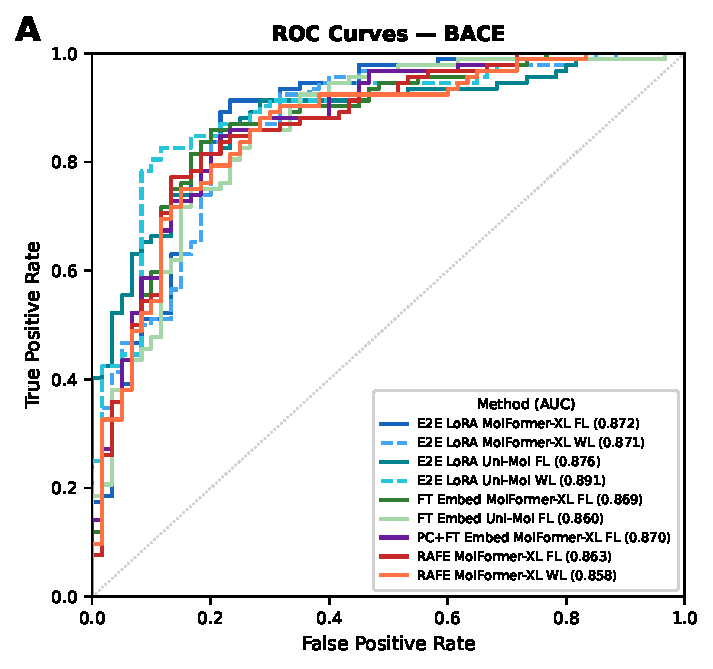
\includegraphics[width=0.49\textwidth]{ Figures_v2/bace_roc.pdf}
%DIFDELCMD <   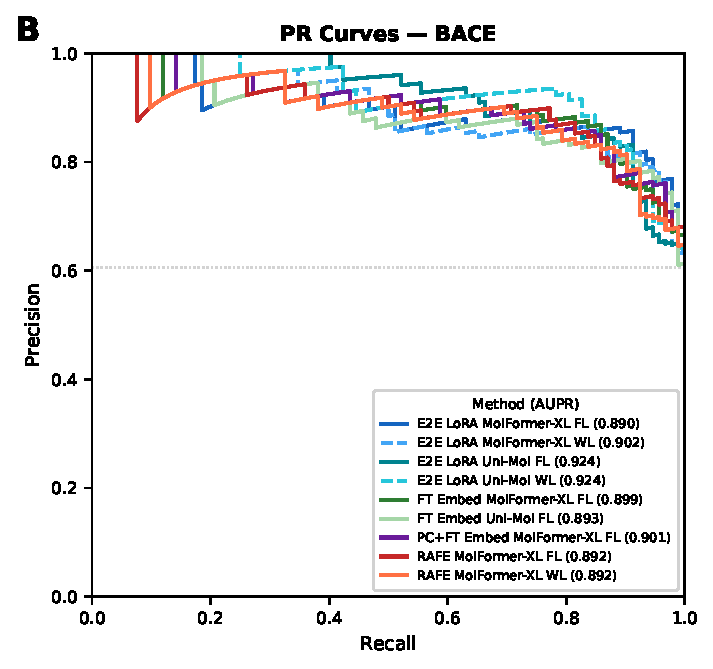
\includegraphics[width=0.49\textwidth]{ Figures_v2/bace_pr.pdf}
%DIFDELCMD <   %%%
%DIFDELCMD < \caption{%
{%DIFAUXCMD
\DIFdelFL{ROC and precision-recall curves for BACE inhibitor prediction. Uni-Mol WL achieves the highest AUPR and overall MCC~$=0.623$.}}
  %DIFAUXCMD
%DIFDELCMD < \label{fig:bace}
%DIFDELCMD < \end{figure*}
%DIFDELCMD < 

%DIFDELCMD < \begin{table*}[ht]
%DIFDELCMD < \centering
%DIFDELCMD < %%%
%DIFDELCMD < \caption{%
{%DIFAUXCMD
\DIFdelFL{Best configurations on BACE. $^*$ overall best by MCC.}}
%DIFAUXCMD
%DIFDELCMD < \label{tab:bace}
%DIFDELCMD < \resizebox{0.95\textwidth}{!}{
%DIFDELCMD < \begin{tabular}{lllllrrrrrrr}
%DIFDELCMD < \toprule
%DIFDELCMD < Modality & CLM & Loss & ML & AUC & Acc & F1$_\text{mac}$ & F1$_\text{mic}$ & MCC & Prec & Rec & SE(MCC) \\
%DIFDELCMD < \midrule
%DIFDELCMD < PC-only    & --- & --- & CatBoost & 0.850 & 0.724 & 0.723 & 0.724 & 0.498 & 0.746 & 0.751 & 0.063 \\
%DIFDELCMD < Chemprop   & --- & --- & --- & 0.855 & 0.763 & 0.759 & 0.763 & 0.528 & 0.758 & 0.770 & 0.068 \\
%DIFDELCMD < GCN        & --- & --- & --- & 0.795 & 0.717 & 0.714 & 0.717 & 0.447 & 0.719 & 0.729 & 0.071 \\
%DIFDELCMD < \midrule
%DIFDELCMD < E2E LoRA   & MolFormer-XL & FL & --- & 0.872 & 0.789 & 0.785 & 0.789 & 0.566 & 0.783 & 0.789 & 0.066 \\
%DIFDELCMD < E2E LoRA$^*$ & Uni-Mol    & WL & --- & \textbf{0.891} & \textbf{0.822} & \textbf{0.808} & \textbf{0.822} & \textbf{0.623} & \textbf{0.823} & \textbf{0.801} & \textbf{0.039} \\
%DIFDELCMD < \midrule
%DIFDELCMD < FT Embed   & MolFormer-XL & FL & CatBoost & 0.869 & 0.763 & 0.762 & 0.763 & 0.557 & 0.773 & 0.784 & 0.062 \\
%DIFDELCMD < RAFE       & MolFormer-XL & WL & LightGBM & 0.858 & 0.770 & 0.768 & 0.770 & 0.561 & 0.774 & 0.787 & 0.040 \\
%DIFDELCMD < \bottomrule
%DIFDELCMD < \end{tabular}
%DIFDELCMD < }
%DIFDELCMD < \end{table*}
%DIFDELCMD < 

%DIFDELCMD < %%%
\DIFdelend \DIFaddbegin \FloatBarrier
\DIFaddend \subsubsection{TDC ADMET Group Results}\label{sec:new_datasets}
This section reports results on the four TDC ADMET Group datasets. All four are evaluated with the same in-house PC-only, Chemprop, and GCN baselines as BACE/BBBP/Flavor.

\paragraph{hERG (Cardiac Ion-Channel Inhibition).} \DIFdelbegin \DIFdel{Table~\ref{tab:herg} }\DIFdelend \DIFaddbegin \DIFadd{Supplementary Table~S5 }\DIFaddend shows results for \DIFdelbegin \DIFdel{the hERG dataset. }\textbf{\DIFdel{Uni-Mol E2E LoRA (WL) is the point-estimate winner}} %DIFAUXCMD
\DIFdel{(}\DIFdelend \DIFaddbegin \DIFadd{hERG (single runs). Uni-Mol E2E LoRA (WL) has the highest value (}\DIFaddend MCC$=0.609$, AUC$=0.881$, SE\DIFdelbegin \DIFdel{$=0.0154$}\DIFdelend \DIFaddbegin \DIFadd{$=0.015$}\DIFaddend ), narrowly ahead of PC-only (MCC$=0.604$, SE\DIFdelbegin \DIFdel{$=0.0157$}\DIFdelend \DIFaddbegin \DIFadd{$=0.016$}\DIFaddend ), FT~Embed+PC (Uni-Mol FL\DIFdelbegin \DIFdel{+ }\DIFdelend \DIFaddbegin \DIFadd{~$+$~}\DIFaddend LightGBM, MCC$=0.602$, SE\DIFdelbegin \DIFdel{$=0.0154$) , }\DIFdelend \DIFaddbegin \DIFadd{$=0.015$) }\DIFaddend and RAFE (Uni-Mol FL\DIFdelbegin \DIFdel{+ }\DIFdelend \DIFaddbegin \DIFadd{~$+$~}\DIFaddend LightGBM, MCC$=0.589$, SE\DIFdelbegin \DIFdel{$=0.0155$). }\textbf{\DIFdel{All four bands overlap at $\pm 1$~SE}}%DIFAUXCMD
\DIFdel{: on hERG's large, well-powered test set }\DIFdelend \DIFaddbegin \DIFadd{$=0.015$). The test set is large }\DIFaddend ($n=2{,}690$), \DIFdelbegin \DIFdel{the absolute MCC gaps are tiny (0.005-0.020)relative to the whisker widths, so this is not a statistically confirmed win for any CLM-based method over the }\DIFdelend \DIFaddbegin \DIFadd{and the controlled comparison shows that RAFE is significantly below }\DIFaddend PC-only \DIFdelbegin \DIFdel{classifier}\DIFdelend \DIFaddbegin \DIFadd{with all three trees (differences $-0.049$, $-0.033$ and $-0.056$ for XGBoost, LightGBM and CatBoost; Table~\ref{tab:controlled}). RAFE is significantly above the fine-tuned embedding alone only with LightGBM ($+0.011$). Over five seeds and the full grid the picture is the same but the margins are smaller (FT Embed }\mHERGFT{}\DIFadd{, FT Embed+PC }\mHERGFTPC{}\DIFadd{, RAFE }\mHERGRAFE{}\DIFadd{, descriptor baseline }\mHERGPC{}\DIFadd{)}\DIFaddend . The full set of ablations \DIFdelbegin \DIFdel{are provided }\DIFdelend \DIFaddbegin \DIFadd{is }\DIFaddend in Supplementary Table~S5.

\DIFdelbegin %DIFDELCMD < \begin{table*}[!ht]
%DIFDELCMD < \centering
%DIFDELCMD < %%%
%DIFDELCMD < \caption{%
{%DIFAUXCMD
\DIFdelFL{Best configurations on hERG (binary, cardiac ion-channel inhibition).}}
%DIFAUXCMD
%DIFDELCMD < \label{tab:herg}
%DIFDELCMD < \resizebox{0.95\textwidth}{!}{
%DIFDELCMD < \begin{tabular}{lllllrrrrrrr}
%DIFDELCMD < \toprule
%DIFDELCMD < Modality & CLM & Loss & ML & AUC & Acc & F1$_\text{mac}$ & MCC & Prec & Rec & SE(MCC) \\
%DIFDELCMD < \midrule
%DIFDELCMD < PC-only     & --- & --- & XGBoost  & 0.874 & 0.802 & 0.802 & 0.604 & 0.802 & 0.802 & 0.0157 \\
%DIFDELCMD < Chemprop    & --- & --- & ---      & 0.854 & 0.779 & 0.779 & 0.558 & 0.779 & 0.779 & 0.0160 \\
%DIFDELCMD < GCN         & --- & --- & ---      & 0.833 & 0.755 & 0.755 & 0.510 & 0.755 & 0.755 & 0.0168 \\
%DIFDELCMD < \midrule
%DIFDELCMD < E2E LoRA    & MolFormer-XL & WL & --- & 0.869 & 0.787 & 0.787 & 0.573 & 0.787 & 0.787 & 0.0155 \\
%DIFDELCMD < E2E LoRA$^*$& Uni-Mol      & WL & --- & \textbf{0.881} & \textbf{0.804} & \textbf{0.804} & \textbf{0.609} & \textbf{0.805} & \textbf{0.804} & \textbf{0.0154} \\
%DIFDELCMD < \midrule
%DIFDELCMD < FT Embed    & Uni-Mol & FL & LightGBM & 0.864 & 0.790 & 0.790 & 0.580 & 0.790 & 0.790 & 0.0158 \\
%DIFDELCMD < FT Embed+PC & Uni-Mol & FL & LightGBM & 0.871 & 0.801 & 0.801 & 0.602 & 0.801 & 0.801 & 0.0154 \\
%DIFDELCMD < RAFE        & Uni-Mol & FL & LightGBM & 0.871 & 0.794 & 0.794 & 0.589 & 0.794 & 0.795 & 0.0155 \\
%DIFDELCMD < \bottomrule
%DIFDELCMD < \end{tabular}
%DIFDELCMD < }
%DIFDELCMD < \end{table*}
%DIFDELCMD < 

%DIFDELCMD < %%%
\DIFdelend \paragraph{DILI (Drug-Induced Liver Injury).} \DIFdelbegin \DIFdel{Table~\ref{tab:dili} }\DIFdelend \DIFaddbegin \DIFadd{Supplementary Table~S6 }\DIFaddend shows results for \DIFdelbegin \DIFdel{the DILI dataset. }\textbf{\DIFdel{RAFE (Uni-Mol FL + XGBoost) is the point-estimate winner}} %DIFAUXCMD
\DIFdel{(}\DIFdelend \DIFaddbegin \DIFadd{DILI (single runs). RAFE (Uni-Mol FL~$+$~XGBoost) has the highest value (}\DIFaddend MCC$=0.790$, AUC$=0.875$, SE\DIFdelbegin \DIFdel{$=0.0515$}\DIFdelend \DIFaddbegin \DIFadd{$=0.051$}\DIFaddend ), ahead of E2E LoRA (ChemBERTa-MTR WL, MCC$=0.770$) and PC-only (MCC$=0.765$, SE\DIFdelbegin \DIFdel{$=0.0581$}\DIFdelend \DIFaddbegin \DIFadd{$=0.058$}\DIFaddend ). This \DIFdelbegin \DIFdel{is the largest absolute point-estimate gap of any dataset in this group ($+0.025$ MCCover }\DIFdelend \DIFaddbegin \DIFadd{single-run value does hold up under repetition: with five seeds, the same configuration gives MCC$=\mDILIRAFE \pm \sDILIRAFE$, FT Embed+PC $\mDILIFTPC \pm \sDILIFTPC$ and }\DIFaddend PC-only \DIFdelbegin \DIFdel{). But DILI's small test set }\DIFdelend \DIFaddbegin \DIFadd{$\mDILIPC$. The test set is small }\DIFaddend ($n=96$)\DIFdelbegin \DIFdel{gives every method a wideSE ($\ge0.05$), and RAFE's $\pm1$~SE band ($0.790\pm0.052$)overlaps PC-only's ($0.765\pm0.058$), so even the largest margin among the four TDC ADMET datasets remains a statistically insignificant win}\DIFdelend \DIFaddbegin \DIFadd{, so every interval is wide. What survives is a consistent benefit of RAFE over the fine-tuned embedding, which is $+0.072$ with XGBoost and $+0.039$ with LightGBM on average over eight embedding and loss combinations (Supplementary Table~S10). Against FT Embed+PC the result depends on the tree model utilized (Supplementary Table~S10)}\DIFaddend . The full set of \DIFdelbegin \DIFdel{ablation results are provided }\DIFdelend \DIFaddbegin \DIFadd{ablations is }\DIFaddend in Supplementary Table~S6.

\DIFdelbegin %DIFDELCMD < \begin{table*}[!ht]
%DIFDELCMD < \centering
%DIFDELCMD < %%%
%DIFDELCMD < \caption{%
{%DIFAUXCMD
\DIFdelFL{Best configurations on DILI (binary, drug-induced liver injury, TDC ADMET Group).}}
%DIFAUXCMD
%DIFDELCMD < \label{tab:dili}
%DIFDELCMD < \resizebox{0.95\textwidth}{!}{
%DIFDELCMD < \begin{tabular}{lllllrrrrrrr}
%DIFDELCMD < \toprule
%DIFDELCMD < Modality & CLM & Loss & ML & AUC & Acc & F1$_\text{mac}$ & MCC & Prec & Rec & SE(MCC) \\
%DIFDELCMD < \midrule
%DIFDELCMD < PC-only     & --- & --- & CatBoost & 0.914 & 0.875 & 0.872 & 0.765 & 0.894 & 0.870 & 0.0581 \\
%DIFDELCMD < Chemprop    & --- & --- & ---      & 0.893 & 0.792 & 0.788 & 0.588 & 0.800 & 0.788 & 0.0808 \\
%DIFDELCMD < GCN         & --- & --- & ---      & 0.889 & 0.854 & 0.850 & 0.729 & 0.880 & 0.849 & 0.0600 \\
%DIFDELCMD < \midrule
%DIFDELCMD < E2E LoRA    & ChemBERTa-MTR & WL & --- & 0.911 & \textbf{0.885} & \textbf{0.885} & 0.770 & 0.886 & \textbf{0.885} & 0.0650 \\
%DIFDELCMD < E2E LoRA    & Uni-Mol       & FL & --- & \textbf{0.926} & 0.854 & 0.854 & 0.708 & 0.855 & 0.853 & 0.0722 \\
%DIFDELCMD < \midrule
%DIFDELCMD < FT Embed    & ChemBERTa-MLM & WL & CatBoost & 0.893 & 0.833 & 0.831 & 0.673 & 0.844 & 0.830 & 0.0731 \\
%DIFDELCMD < FT Embed+PC & Uni-Mol       & FL & LightGBM & 0.873 & 0.833 & 0.826 & 0.703 & 0.879 & 0.826 & 0.0552 \\
%DIFDELCMD < RAFE$^*$    & Uni-Mol       & FL & XGBoost  & 0.875 & \textbf{0.885} & 0.883 & \textbf{0.790} & \textbf{0.910} & 0.880 & \textbf{0.0515} \\
%DIFDELCMD < \bottomrule
%DIFDELCMD < \end{tabular}
%DIFDELCMD < }
%DIFDELCMD < \end{table*}
%DIFDELCMD < 

%DIFDELCMD < %%%
\DIFdel{Figures~\ref{fig:roc_4ds} and ~\ref{fig:pr_4ds} summarize }\DIFdelend \DIFaddbegin \DIFadd{Supplementary Figure~S2 summarizes the ROC and precision-recall behaviour of }\DIFaddend the four tree-based modalities (PC-only, FT Embed, FT Embed+PC, RAFE) \DIFdelbegin \DIFdel{across all }\DIFdelend \DIFaddbegin \DIFadd{on the }\DIFaddend four binary classification datasets, and two things stand out. First, on hERG the four ROC and PR curves are nearly superimposed (AUC $0.864$-$0.874$, AUPR $0.862$-$0.872$), \DIFdelbegin \DIFdel{consistent with the $\pm1$~SE overlap already reported: none of the tree-based modalities separates meaningfully from PC-only on this large, well-powered test set}\DIFdelend \DIFaddbegin \DIFadd{so the modalities do not separate on AUC even though the paired MCC comparison finds RAFE below PC-only}\DIFaddend . Second, RAFE's rank\DIFdelbegin \DIFdel{ing}\DIFdelend  among the tree-based modalities \DIFdelbegin \DIFdel{is dataset-dependent rather than uniformly best}\DIFdelend \DIFaddbegin \DIFadd{depends on the dataset}\DIFaddend . It is the top tree-based modality on BBBP (AUC$=0.940$, AUPR$=0.940$) \DIFdelbegin \DIFdel{, but on BACE it is }\DIFdelend \DIFaddbegin \DIFadd{and }\DIFaddend the weakest of the four \DIFaddbegin \DIFadd{on BACE for the configurations shown }\DIFaddend (AUC$=0.858$, \DIFdelbegin \DIFdel{trailing }\DIFdelend \DIFaddbegin \DIFadd{against $0.869$ and $0.870$ for }\DIFaddend FT Embed and FT Embed+PC\DIFdelbegin \DIFdel{at $0.869$-$0.870$). That is fitting, since BACE's confirmed win traces back to the 3D Uni-Mol E2E LoRA model, not to tree-based RAFE. DILI shows the largest divergence between the two curve types: PC-only's AUC margin over RAFE is modest ($0.914$ vs.\ }\DIFdelend \DIFaddbegin \DIFadd{). The curves show each modality's best configuration by MCC; ranked by AUC instead, the best RAFE configuration on BACE reaches }\DIFaddend $0.875$ \DIFdelbegin \DIFdel{), but its AUPR margin is substantially larger ($0.911$ vs.\ $0.847$). This shows that on this small ($n=96$), imbalanced test set PC-only's precision-recall trade-off is more favorable than ROC-AUC alone would suggest, even though RAFE remains the point-estimate MCC winner in Table~\ref{tab:dili}}\DIFdelend \DIFaddbegin \DIFadd{(Supplementary Table~S4)}\DIFaddend . 


\DIFdelbegin %DIFDELCMD < \begin{figure*}[!ht]
%DIFDELCMD <   \centering
%DIFDELCMD <   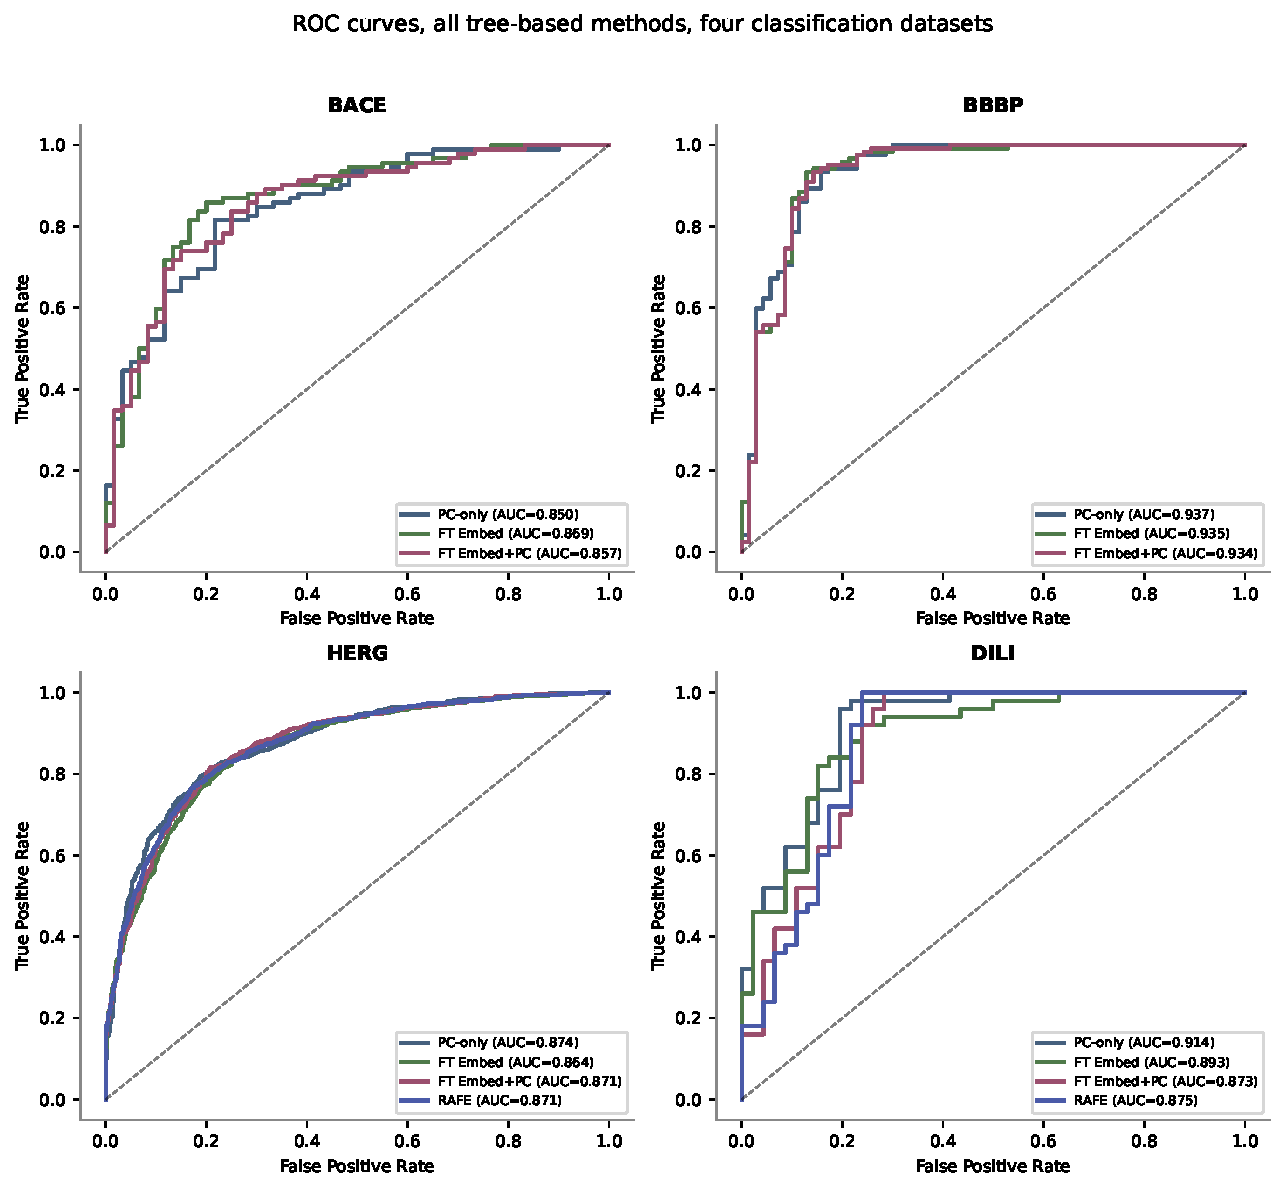
\includegraphics[width=0.95\textwidth]{ Figures_v2/roc_curves_4datasets.pdf}
%DIFDELCMD <   %%%
%DIFDELCMD < \caption{%
{%DIFAUXCMD
\DIFdelFL{ROC curves for best configuration of tree-based methods (PC-only, FT Embed, FT Embed+PC and RAFE), on all four binary classification datasets in this study: two MoleculeNet (BACE, BBBP) and two TDC ADMET tasks (hERG, DILI).}}
  %DIFAUXCMD
%DIFDELCMD < \label{fig:roc_4ds}
%DIFDELCMD < \end{figure*}
%DIFDELCMD < 

%DIFDELCMD < \begin{figure*}[!ht]
%DIFDELCMD <   \centering
%DIFDELCMD <   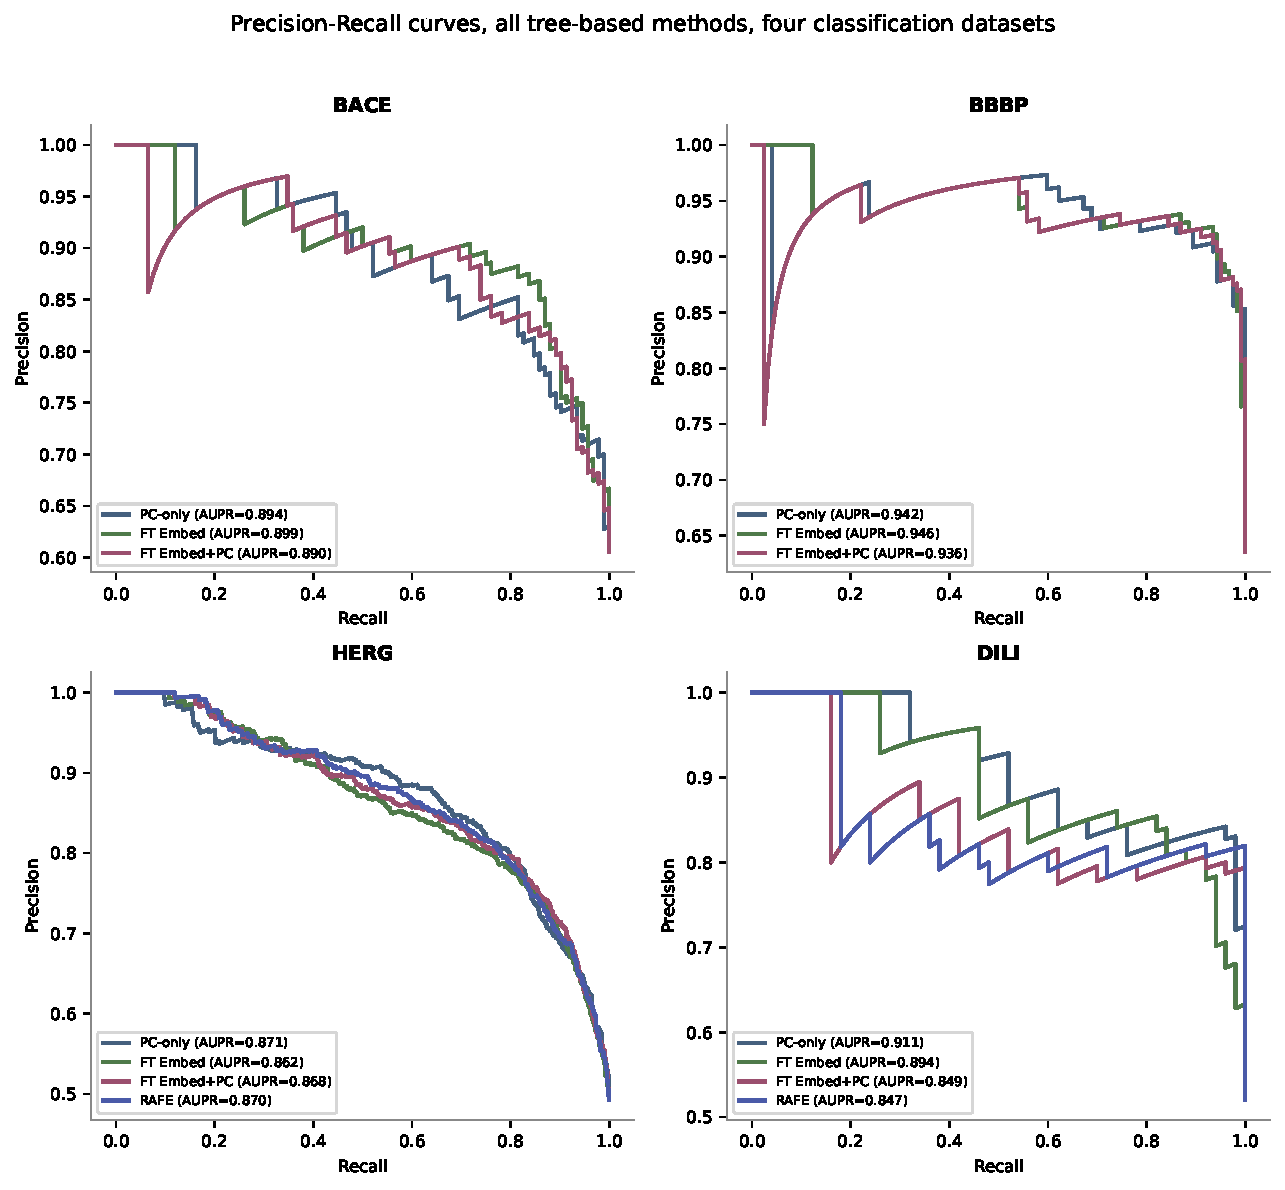
\includegraphics[width=0.95\textwidth]{ Figures_v2/pr_curves_4datasets.pdf}
%DIFDELCMD <   %%%
%DIFDELCMD < \caption{%
{%DIFAUXCMD
\DIFdelFL{Precision-recall curves for the same models and datasets as Figure~\ref{fig:roc_4ds}. DILI's small test set ($n=96$) produces visibly noisier curves than the other three datasets, consistent with its wide bootstrapped SE throughout this paper.}}
  %DIFAUXCMD
%DIFDELCMD < \label{fig:pr_4ds}
%DIFDELCMD < \end{figure*}
%DIFDELCMD < 

%DIFDELCMD < %%%
\DIFdelend \DIFaddbegin \FloatBarrier
\DIFaddend \paragraph{Caco-2 Permeability (Regression).} \DIFdelbegin \DIFdel{Table~\ref{tab:caco2} shows the results on the }\DIFdelend \DIFaddbegin \DIFadd{Supplementary Table~S7 shows the }\DIFaddend Caco-2 \DIFdelbegin \DIFdel{dataset}\DIFdelend \DIFaddbegin \DIFadd{results (single runs)}\DIFaddend , ranked by Spearman correlation. \DIFdelbegin \textbf{\DIFdel{PC-only is the overall winner}} %DIFAUXCMD
\DIFdelend \DIFaddbegin \DIFadd{PC-only has the highest value }\DIFaddend (Spearman$=0.853$, R\textsuperscript{2}$=0.744$, SE$=0.021$), ahead of RAFE (ChemBERTa-MTR\DIFdelbegin \DIFdel{+ }\DIFdelend \DIFaddbegin \DIFadd{~$+$~}\DIFaddend CatBoost, Spearman$=0.835$, R\textsuperscript{2}$=0.663$, SE$=0.026$) and FT~Embed+PC (Spearman$=0.824$, R\textsuperscript{2}$=0.672$). \DIFdelbegin \DIFdel{Every CLM-based method's band overlaps }\DIFdelend \DIFaddbegin \DIFadd{Five-seed means tell the same story: $\mCACORAFE$ for RAFE, $\mCACOFTPC$ for FT Embed+PC, $\mCACOFT$ for FT Embed and $\mCACOPC$ for }\DIFaddend PC-only\DIFdelbegin \DIFdel{'s at $\pm1$~SE. This is the clearest example of a task where a purely engineered physicochemical feature set (i.e.\ logP-adjacent descriptors, }\DIFdelend \DIFaddbegin \DIFadd{. The clear effect on Caco-2 is the gain of RAFE and of FT Embed+PC over the fine-tuned embedding alone ($+0.084$ for LightGBM; 95\% interval $+0.059$ to $+0.111$, Supplementary Table~S10). Most of that gain is already provided by the descriptors, which are }\DIFaddend mechanistically close to membrane permeability\DIFdelbegin \DIFdel{) outperforms }\DIFdelend \DIFaddbegin \DIFadd{, and a descriptor-only model matches or exceeds }\DIFaddend every CLM-based \DIFdelbegin \DIFdel{representation, echoing the pattern already documented for Flavor. A }\DIFdelend \DIFaddbegin \DIFadd{stage. The }\DIFaddend full set of ablation results is \DIFdelbegin \DIFdel{available }\DIFdelend in Supplementary Table~S7.

\DIFdelbegin %DIFDELCMD < \begin{table*}[!ht]
%DIFDELCMD < \centering
%DIFDELCMD < %%%
%DIFDELCMD < \caption{%
{%DIFAUXCMD
\DIFdelFL{Best configurations on Caco-2 permeability (regression, TDC ADMET Group), ranked by Spearman.}}
%DIFAUXCMD
%DIFDELCMD < \label{tab:caco2}
%DIFDELCMD < \resizebox{0.95\textwidth}{!}{
%DIFDELCMD < \begin{tabular}{lllrrrr}
%DIFDELCMD < \toprule
%DIFDELCMD < Modality & CLM & ML & R\textsuperscript{2} & MAE & Spearman & SE(Spearman) \\
%DIFDELCMD < \midrule
%DIFDELCMD < PC-only$^*$ & --- & CatBoost & 0.744 & 0.273 & \textbf{0.853} & \textbf{0.0211} \\
%DIFDELCMD < Chemprop    & --- & --- & 0.534 & 0.359 & 0.802 & 0.0294 \\
%DIFDELCMD < GCN         & --- & --- & 0.244 & 0.491 & 0.733 & 0.0342 \\
%DIFDELCMD < \midrule
%DIFDELCMD < E2E LoRA    & ChemBERTa-MTR & --- & 0.622 & 0.340 & 0.789 & 0.0318 \\
%DIFDELCMD < E2E LoRA    & Uni-Mol       & --- & 0.411 & 0.432 & 0.580 & 0.0565 \\
%DIFDELCMD < \midrule
%DIFDELCMD < FT Embed    & ChemBERTa-MTR & CatBoost & \textbf{0.668} & 0.318 & 0.821 & 0.0284 \\
%DIFDELCMD < FT Embed+PC & ChemBERTa-MTR & LightGBM & 0.672 & \textbf{0.308} & 0.824 & 0.0277 \\
%DIFDELCMD < RAFE        & ChemBERTa-MTR & CatBoost & 0.663 & 0.324 & 0.835 & 0.0256 \\
%DIFDELCMD < \bottomrule
%DIFDELCMD < \end{tabular}
%DIFDELCMD < }
%DIFDELCMD < \end{table*}
%DIFDELCMD < 

%DIFDELCMD < %%%
\DIFdelend \paragraph{Half-Life (Regression).} \DIFdelbegin \DIFdel{Table~\ref{tab:half_life} reports results for the }\DIFdelend \DIFaddbegin \DIFadd{Supplementary Table~S8 reports }\DIFaddend Half-Life \DIFdelbegin \DIFdel{dataset, again }\DIFdelend \DIFaddbegin \DIFadd{results (single runs), }\DIFaddend ranked by Spearman correlation. \DIFdelbegin \textbf{\DIFdel{FT Embed (MolFormer-XL + XGBoost) is the point-estimate winner}} %DIFAUXCMD
\DIFdel{(}\DIFdelend \DIFaddbegin \DIFadd{FT Embed (MolFormer-XL~$+$~XGBoost) has the highest value (}\DIFaddend Spearman$=0.600$, R\textsuperscript{2}$=0.083$, SE$=0.056$), ahead of FT~Embed+PC (Spearman$=0.593$) and PC-only (Spearman$=0.502$, SE$=0.075$). Half-Life is the noisiest dataset ($n_\text{test}=133$, R\textsuperscript{2} \DIFdelbegin \DIFdel{$< 0.11$ }\DIFdelend \DIFaddbegin \DIFadd{$\le 0.114$ }\DIFaddend for every method after log1p transformation and outlier removal)\DIFdelbegin \DIFdel{; the $\pm1$~SE }\DIFdelend \DIFaddbegin \DIFadd{, and the }\DIFaddend bands of FT Embed and PC-only overlap\DIFdelbegin \DIFdel{substantially, so despite a $+0.098$ Spearman point-estimate gap this is not a confirmed win}\DIFdelend \DIFaddbegin \DIFadd{. RAFE is not favorable here: with LightGBM it is below FT Embed+PC ($-0.023$, 95\% interval $-0.044$ to $-0.002$). Spearman and R\textsuperscript{2} behave differently on this dataset, as discussed in Section~\ref{sec:metrics}}\DIFaddend . The full per-embedding, per-loss ablation is \DIFdelbegin \DIFdel{detailed }\DIFdelend in Supplementary Table~S8.

\DIFdelbegin %DIFDELCMD < \begin{table*}[!ht]
%DIFDELCMD < \centering
%DIFDELCMD < %%%
%DIFDELCMD < \caption{%
{%DIFAUXCMD
\DIFdelFL{Best configurations on drug Half-Life (regression, TDC ADMET Group, log1p target), ranked by Spearman.}}
%DIFAUXCMD
%DIFDELCMD < \label{tab:half_life}
%DIFDELCMD < \resizebox{0.95\textwidth}{!}{
%DIFDELCMD < \begin{tabular}{lllrrrr}
%DIFDELCMD < \toprule
%DIFDELCMD < Modality & CLM & ML & R\textsuperscript{2} & MAE (h) & Spearman & SE(Spearman) \\
%DIFDELCMD < \midrule
%DIFDELCMD < PC-only     & --- & XGBoost & 0.110 & 5.687 & 0.502 & 0.0750 \\
%DIFDELCMD < Chemprop    & --- & --- & -0.020 & 6.325 & 0.332 & 0.0841 \\
%DIFDELCMD < GCN         & --- & --- & 0.114 & 5.928 & 0.418 & 0.0777 \\
%DIFDELCMD < \midrule
%DIFDELCMD < E2E LoRA    & ChemBERTa-MTR & --- & 0.072 & 6.367 & 0.541 & 0.0654 \\
%DIFDELCMD < E2E LoRA    & Uni-Mol       & --- & -0.072 & 6.937 & 0.518 & 0.0720 \\
%DIFDELCMD < \midrule
%DIFDELCMD < FT Embed$^*$& MolFormer-XL & XGBoost & \textbf{0.083} & \textbf{5.639} & \textbf{0.600} & \textbf{0.0562} \\
%DIFDELCMD < FT Embed+PC & MolFormer-XL & XGBoost & 0.090 & 5.594 & 0.593 & 0.0535 \\
%DIFDELCMD < RAFE        & MolFormer-XL & XGBoost & 0.090 & 5.557 & 0.568 & 0.0579 \\
%DIFDELCMD < \bottomrule
%DIFDELCMD < \end{tabular}
%DIFDELCMD < }
%DIFDELCMD < \end{table*}
%DIFDELCMD < %%%
\DIFdelend \DIFaddbegin \FloatBarrier
\subsection{\DIFadd{Controlled Comparison of Representations}}\label{sec:controlled}
\DIFadd{The single-run tables compare the best row of each mode, and these rows can come from different tree models. To separate the effect of the representation from that of the tree, we ran PC-only, FT Embed, FT Embed+PC and RAFE with the same code, splits, test molecules, tuning budget, three tree models and five seeds, for one embedding configuration per dataset (two for BACE; Table~\ref{tab:controlled}, Figure~\ref{fig:matrix}).
}\DIFaddend 

\DIFdelbegin \subsection{\DIFdel{Effectiveness of RAFE: Does Retrieval Substitute for 3D Geometry?}}%DIFAUXCMD
\addtocounter{subsection}{-1}%DIFAUXCMD
%DIFDELCMD < \label{sec:rafe_effectiveness}
%DIFDELCMD < %%%
\DIFdel{RAFE is the point-estimate winner on BBBP (MCC$=0.798$) and DILI (MCC$=0.790$), and competitive with E2E LoRA and FT Embed}\DIFdelend \DIFaddbegin \DIFadd{Three results follow. First, RAFE is never significantly better or worse than FT Embed}\DIFaddend +\DIFdelbegin \DIFdel{PC elsewhere. Its gain }\DIFdelend \DIFaddbegin \DIFadd{PC: none of the 24 paired comparisons (eight dataset configurations, three trees) has an interval that excludes zero. Second, RAFE is significantly better than FT Embed alone in 5 of 24 comparisons (Caco-2 with all three trees, DILI with XGBoost and hERG with LightGBM) and never worse. Third, RAFE is significantly below PC-only in 4 of 24 comparisons (hERG with all three trees, Flavor with XGBoost) and never significantly above it. The point estimates favor the fine-tuned stages }\DIFaddend over PC-only \DIFdelbegin \DIFdel{is closest to statistically confirmed on BBBP}\DIFdelend \DIFaddbegin \DIFadd{on BACE (MolFormer), BBBP, DILI and Half-Life, whereas PC-only is highest or tied on Caco-2, hERG and Flavor; none of the former differences is significant.
}

\DIFadd{Across the matched embedding-loss-tree configurations of the supplementary tables, RAFE exceeds FT Embed on four of seven datasets (BBBP $+0.014$, Wilcoxon $p=0.025$; hERG $+0.006$}\DIFaddend , \DIFdelbegin \DIFdel{where the $\pm1$~SE bands ($0.798\pm0.028$ vs. \ $0.759\pm0.043$) are close to non-overlapping; on DILI}\DIFdelend \DIFaddbegin \DIFadd{$p=0.015$; DILI $+0.052$}\DIFaddend , \DIFdelbegin \DIFdel{hERG, }\DIFdelend \DIFaddbegin \DIFadd{$p=0.012$; }\DIFaddend Caco-2 \DIFaddbegin \DIFadd{$+0.085$}\DIFaddend , \DIFaddbegin \DIFadd{$p<0.001$; Figure~\ref{fig:ladder}). These tests are descriptive, because the configurations share one test set. Figure~\ref{fig:pareto} places the same stages on a cost-performance axis: the retrieval stage joins the Pareto frontier only on the datasets where it clears the cheaper stage by more than $0.005$.
}

\begin{table*}[!ht]
\centering
\caption{\DIFaddFL{Controlled comparison: mean test metric over five seeds for each representation, tree model and dataset (one embedding configuration per dataset; MCC for classification, Spearman for regression). Every row uses identical splits, test molecules and tuning budget.}}
\label{tab:controlled}
\footnotesize
\input{tables/tab_controlled_v5.tex}
\end{table*}

\begin{figure*}[!ht]
  \centering
  \begin{subfigure}[t]{\textwidth}
    \centering
    \includegraphics[width=0.95\textwidth]{controlled_matrix_v3.pdf}
    \caption{}
    \label{fig:matrix}
  \end{subfigure}
  \par\bigskip
  \begin{subfigure}[t]{\textwidth}
    \centering
    \includegraphics[width=0.75\textwidth]{ladder_gain_v3.pdf}
    \caption{}
    \label{fig:ladder}
  \end{subfigure}
  \caption{\DIFaddFL{Controlled comparison of the PEARL stages. Both panels use the primary ranking metric (MCC, or Spearman for Caco-2 and Half-Life).
  }\textbf{\DIFaddFL{(a)}} \DIFaddFL{The comparison of Table~\ref{tab:controlled}, one panel per dataset configuration (BACE appears twice, for its MolFormer and its Uni-Mol embedding). The horizontal axis steps through the four representations in ladder order and the vertical axis is the five-seed mean; the thick bar is the mean over the three trees and the black markers are the individual trees (circle XGBoost, square LightGBM, triangle CatBoost). Splits, test molecules, tuning budget and seeds are identical at every point.
  }\textbf{\DIFaddFL{(b)}} \DIFaddFL{Mean difference between stages, one row per dataset, over the embedding-loss-tree configurations matched across both stages in the supplementary tables: FT Embed$+$PC versus FT Embed, RAFE versus FT Embed, and RAFE versus FT Embed$+$PC. Bars are 95\% bootstrap intervals over configurations, so a bar crossing the zero line indicates no detectable difference. These intervals are descriptive, because the configurations share one test set.}}
  \label{fig:controlled_comparison}
\end{figure*}

\begin{figure*}[!ht]
  \centering
  \includegraphics[width=0.95\textwidth]{pareto_frontier_v3.pdf}
  \caption{\DIFaddFL{Cost-performance view of the PEARL ladder, one panel per dataset. The horizontal axis is the added pipeline cost along the frozen-embedding ladder (FT Embed $\rightarrow$ $+$PC $\rightarrow$ $+$RAFE) and the vertical axis is the best configuration of each stage, labelled with the embedding, loss and tree that produced it; the faint dots behind each stage are all of its configurations. The black staircase is the Pareto frontier, which a stage joins only by exceeding every cheaper stage by more than $0.005$ (filled marker: on the frontier, hollow marker: dominated by a cheaper stage), and the green dashed line is the best end-to-end LoRA value for reference. Unlike Figure~\ref{fig:controlled_comparison}, this figure uses the single-run values of the supplementary tables, and the inset panel restates how to read it.}}
  \label{fig:pareto}
\end{figure*}

\paragraph{\DIFadd{Full same-tree tables.}} \DIFadd{Table~\ref{tab:controlled} uses one embedding per dataset. Supplementary Table~S10 extends the comparison to the full grid for the datasets on which RAFE is most often discussed (DILI, Caco-2 and BBBP, alongside BACE }\DIFaddend and Half-Life\DIFaddbegin \DIFadd{): every embedding and loss combination, with the three stages compared inside one tree. The bottom rows give the difference pooled over rows and seeds with a paired interval. On DILI, RAFE exceeds FT Embed with both trees (XGBoost $+0.072$}\DIFaddend , \DIFdelbegin \DIFdel{RAFE's (or another method's)point-estimate win over }\DIFdelend \DIFaddbegin \DIFadd{95\% interval $+0.036$ to $+0.111$; LightGBM $+0.039$, $+0.002$ to $+0.076$). Against FT Embed+PC the result depends on the tree: with XGBoost the pooled difference is $+0.032$ ($+0.005$ to $+0.060$), and with LightGBM it is $-0.009$ ($-0.029$ to $+0.012$). On Caco-2, RAFE and FT Embed+PC are indistinguishable and both exceed FT Embed (LightGBM: $+0.084$, $+0.059$ to $+0.111$), while }\DIFaddend PC-only \DIFdelbegin \DIFdel{does not survive a $\pm1$~SE overlap test. Figures~\ref{fig:roc_4ds} and ~\ref{fig:pr_4ds} (Section~\ref{sec:new_datasets}) further show that RAFE's ranking among the tree-based modalities is itself dataset-dependent}\DIFdelend \DIFaddbegin \DIFadd{exceeds every CLM-based stage. On BBBP, no stage separates from another with any tree. All three tree models are included in these tables.
}

\FloatBarrier
\subsection{\DIFadd{Best Configuration per Dataset on Five-Seed Means}}\label{sec:best_configs}
\DIFadd{PEARL is a configuration benchmark: for each dataset the question is which embedding, loss, tree and stage works best. Because the best of many configurations is optimistic when taken from one run, we repeated the full configuration grid with five seeds for all three tree models on all seven datasets (Figure~\ref{fig:grid}), which is 24 configurations per stage for the classification tasks and 12 for the regression tasks. Table~\ref{tab:best_configs} lists the best configuration of each stage by five-seed test mean alongside the single-run value of the same modality in the original tables, and Table~\ref{tab:runnerup} gives the runner-up configuration of the same cell and the paired difference between the two.
}

\DIFadd{Three observations follow. The best configuration is MolFormer in }\nmf{} \DIFadd{of }\nrows{} \DIFadd{rows, and the single-run values of the original tables exceed the five-seed means in }\nsr{} \DIFadd{of }\nrows{} \DIFadd{rows; the largest drop is for DILI RAFE, from 0.790 to }\mDILIRAFE{}\DIFadd{. The best configuration is separable from the runner-up in only }\nsep{} \DIFadd{of }\nrows{} \DIFadd{rows, so the identity of the best configuration is itself uncertain and claims should rest on paired differences. Selecting the configuration by training-split cross-validation is unreliable on these scaffold splits: it lowers the RAFE score by }\gaplo{} \DIFadd{to }\gaphi{} \DIFadd{(MCC or Spearman) relative to the test-based choice, and we do not use it for ranking.
}

\DIFadd{Ranking the best configuration of each of seven methods across all }\nds{} \DIFadd{datasets, RAFE is in the top three on }\ntop{} \DIFadd{of }\nds{} \DIFadd{with a mean rank of }\mrankRAFE{}\DIFadd{. FT Embed+PC has mean rank }\mrankFTPC{}\DIFadd{, PC-only }\mrankPC{} \DIFadd{and FT Embed }\mrankFT{}\DIFadd{. The three leading stages are separated by less than half a rank. A seven-way ranking over seven datasets cannot resolve a margin of that size. On five of the seven datasets the gap between RAFE and the method immediately above it is smaller than RAFE's own seed-to-seed standard deviation. The single-run best values of the original tables give a more favorable picture for RAFE}\DIFaddend : it is \DIFdelbegin \DIFdel{the strongest tree-based modality on BBBP but the weakest of the four on BACE.
}\DIFdelend \DIFaddbegin \DIFadd{first on BBBP and DILI and in the top three on }\srtop{} \DIFadd{of seven datasets (Supplementary Figure~S3).
}\DIFaddend 

\DIFdelbegin \DIFdel{We observe that RAFE 's }\DIFdelend \DIFaddbegin \DIFadd{One caveat applies to every ranking we report. The four stages we ran ourselves (FT Embed, FT Embed+PC, RAFE and PC-only) are five-seed means. The external references (end-to-end LoRA, Chemprop and GCN) are single runs carried over from the original tables, since repeating them with independent seeds was beyond our budget. A single run reports the best value observed rather than an expected value, so the external baselines are measured on a more favorable basis than our own stages, and the comparison is conservative with respect to RAFE. We therefore treat the paired comparisons of Section~\ref{sec:controlled}, which change one component at a time on identical molecules, as the primary evidence and the ranking as context.
}

\begin{table*}[!ht]
\centering
\caption{\DIFaddFL{Best configuration per dataset and stage, judged on five-seed test means (XGBoost and LightGBM). ``Single run'' is the best value of the same modality in the original tables. Table~\ref{tab:runnerup} gives the runner-up configuration of each row and the paired difference to it.}}
\label{tab:best_configs}
\footnotesize
\input{tables/tab_best_configs_v5.tex}
\end{table*}

\begin{table*}[!ht]
\centering
\caption{\DIFaddFL{Runner-up configuration for each row of Table~\ref{tab:best_configs}, with the difference between the best and the runner-up configuration and its paired 95\% bootstrap interval. Bold marks the one row whose interval excludes zero.}}
\label{tab:runnerup}
\footnotesize
\input{tables/tab_runnerup_v5.tex}
\end{table*}

\begin{figure*}[!ht]
  \centering
  \includegraphics[width=0.99\textwidth]{grid_heatmap_v5.pdf}
  \caption{\DIFaddFL{Five-seed mean test metric over the full configuration grid, for all seven datasets (one panel each, the seventh centred below the two full rows). Within a panel, rows are embedding and loss combinations and columns are the nine stage-by-tree cells (FT Embed, FT Embed$+$PC and RAFE, each with XGBoost, LightGBM and CatBoost); colour and the printed value give the five-seed mean of MCC, or of Spearman for Caco-2 and Half-Life. The red box marks the best cell of that dataset. Each panel has its own colour scale, so colours are comparable within a dataset but not across datasets.}}
  \label{fig:grid}
\end{figure*}

\FloatBarrier
\subsection{\DIFadd{Conventional Fingerprints and Descriptors}}\label{sec:fingerprints}
\DIFadd{Table~\ref{tab:fingerprints} evaluates ECFP4, ECFP6, MACCS, ECFP4$+$MACCS, the RDKit descriptors and the 473 physicochemical descriptors with the same trees and tuning (best tree shown). Fingerprints alone are clearly weaker than descriptors on Caco-2 (}\ecfpcaco{} \DIFadd{for ECFP4 versus }\pccaco{}\DIFadd{), DILI and Half-Life, and comparable on BACE, hERG and Flavor. RAFE is clearly better than ECFP4 alone on DILI ($+\draferecfpdili$) and Caco-2 ($+\draferecfpcaco$). Against PC-only the paired intervals include zero on BBBP, DILI and Caco-2, the three datasets compared.
}

\begin{table}[!ht]
\centering
\caption{\DIFaddFL{Fingerprint and descriptor baselines (best tree per cell; MCC for classification, Spearman for regression). Three seeds on the smaller datasets and one on hERG and Flavor.}}
\label{tab:fingerprints}
\footnotesize
\input{tables/tab_fingerprints_v5.tex}
\end{table}

\FloatBarrier
\subsection{\DIFadd{What Does RAFE Add?}}\label{sec:rafe_effectiveness}
\DIFadd{This section addresses H2. We examine which RAFE components matter, how sensitive RAFE is to its retrieval settings, what it adds to the embedding and descriptors, and whether }\DIFaddend label-free \DIFaddbegin \DIFadd{variants change the conclusion.
}

\paragraph{\DIFadd{Feature groups.}} \DIFadd{Adding or removing any of the four RAFE groups changes the score by no more than 0.02 in }\fracsmall\DIFadd{\% of the }\ncellsabl{} \DIFadd{dataset-by-arm cells (Table~\ref{tab:groups}, Figure~\ref{fig:groups}). The }\nbig{} \DIFadd{larger shifts are all decreases and are confined to }\bigcfg{}\DIFadd{, which have the smallest test sets in the study. No single group is responsible for the effect of RAFE, which is consistent with the groups carrying overlapping information.
}

\begin{table*}[!ht]
\centering
\caption{\DIFaddFL{RAFE feature-group ablation (five-seed means, each dataset at its own tree). Columns under ``Added to FT$+$PC'' add one group to FT Embed+PC; columns under ``Removed from RAFE'' drop one group from full RAFE. A: physicochemical neighborhood, B: density, C: centroid, D: Tanimoto.}}
\label{tab:groups}
\scriptsize
\adjustbox{max width=\textwidth}{\input{tables/tab_groups_v5.tex}}
\end{table*}

\FloatBarrier
\paragraph{\DIFadd{Retrieval metric and neighbor count.}} \DIFadd{We compared CLM-cosine retrieval with Morgan-Tanimoto retrieval and with random retrieval (five independent random draws), and swept $k$ from 1 to 100. Of }\nkcomp{} \DIFadd{paired comparisons, }\nkexc{} \DIFadd{have an interval that excludes zero (}\excdetails\DIFadd{; Figure~\ref{fig:retrieval}), and both differences are below 0.011 in size. RAFE therefore does not need its retrieval settings tuned. Random neighbors perform as well as similar ones, which shows that RAFE acts as chemical-space context and not as an analogue lookup. The neighbor-count sweep covers every dataset, BBBP included, and no value of $k$ separates from $k=10$ on any of them.
}

\begin{figure}[!ht]
  \centering
  \begin{subfigure}[t]{\textwidth}
    \centering
    \includegraphics[width=0.99\textwidth]{ablation_groups_v3.pdf}
    \caption{}
    \label{fig:groups}
  \end{subfigure}
  \par\bigskip
  \begin{subfigure}[t]{\textwidth}
    \centering
    \includegraphics[width=0.99\textwidth]{retrieval_robustness_v3.pdf}
    \caption{}
    \label{fig:retrieval}
  \end{subfigure}
  \caption{\DIFaddFL{RAFE ablation controls. }\textbf{\DIFaddFL{(a)}} \DIFaddFL{Change relative to FT Embed+PC for each feature-group arm (RAFE-X: RAFE without group X). }\textbf{\DIFaddFL{(b)}} \DIFaddFL{Left: effect of the number of retrieved neighbors (difference to $k=10$). Right: effect of the retrieval strategy (difference to CLM-cosine retrieval; error bars show the spread over the five random draws).}}
  \label{fig:rafe_ablation}
\end{figure}

\FloatBarrier
\paragraph{\DIFadd{Complementarity with the embedding and descriptors.}} \DIFadd{The per-molecule gain of RAFE over FT Embed+PC is unrelated to }\DIFaddend ZINC-250k \DIFdelbegin \DIFdel{neighborhood context (see Supplementary Table~S10)is a genuinely useful, orthogonal signal on tasks like BBBP where bulk physicochemical neighborhood properties (e.g.\ logP)are mechanistically related to }\DIFdelend \DIFaddbegin \DIFadd{coverage (Spearman correlation between }\spmin{} \DIFadd{and }\spmax{} \DIFadd{across datasets; all intervals include zero; Figure~\ref{fig:e10}, left). A ridge model recovers }\rgAlo{} \DIFadd{to }\rgAhi\DIFadd{\% of the variance of the physicochemical-neighborhood group, }\rgBlo{} \DIFadd{to }\rgBhi\DIFadd{\% of the density group and }\rgClo{} \DIFadd{to }\rgChi\DIFadd{\% of the centroid group from the embedding and descriptors on held-out molecules (a linear estimate), so these groups are partly complementary and partly redundant. The Tanimoto group is not predictable from them (Figure~\ref{fig:e10}, right). RAFE corrects or breaks between 0 and }\ecorrmax{} \DIFadd{test molecules on the classification sets, so it acts as a conservative refinement.
}

\begin{figure}[!ht]
  \centering
  \includegraphics[width=0.99\textwidth]{rafe_complementarity_v3.pdf}
  \caption{\DIFaddFL{Left: per-molecule gain of RAFE over FT Embed+PC by ZINC-250k coverage tercile. Right: held-out R\textsuperscript{2} of each RAFE group predicted from the embedding and the descriptors.}}
  \label{fig:e10}
\end{figure}

\FloatBarrier
\paragraph{\DIFadd{Label-free variants.}} \DIFadd{To test whether the redundant part of RAFE can be removed, we evaluated five variants that use no labels in retrieval or feature construction: groups A and B only (V1), residualized features (V2), additional ZINC-250k properties (V3), compressed features (V4) and hybrid retrieval (V5) (Supplementary Table~S12). Of }\vn{} \DIFadd{paired comparisons of the variants with FT Embed+PC (}\nvards{} \DIFadd{datasets, two trees), }\vbetterft{} \DIFadd{is significantly better and }\vworseft{} \DIFadd{significantly worse. Against RAFE, }\vbetterrf{} \DIFadd{are better and }\vworserf{} \DIFadd{worse. No variant improves on RAFE, which supports the reading of RAFE as a conservative refinement.
}

\FloatBarrier
\subsection{\DIFadd{Coverage of the Chemical Space by ZINC-250k}}\label{sec:coverage}
\DIFadd{For every dataset molecule we computed the largest Morgan-Tanimoto similarity to ZINC-250k (Table~\ref{tab:coverage}). The median is }\covmedian{} \DIFadd{over all }\covn{} \DIFadd{molecules, and about }\covsixty\DIFadd{\% have a neighbor at 0.6 or above; BACE is the least covered (median }\covbace{}\DIFadd{). Figure~\ref{fig:umap} shows the same picture qualitatively: each dataset occupies a region of the joint UMAP embedding that overlaps the ZINC-250k subsample without being densely covered by it, and the per-dataset similarity distributions in the last panel concentrate below 0.5. ZINC-250k therefore provides background chemical context and not close analogues. This agrees with the result that random neighbors perform like similar ones and that the per-molecule gain does not depend on coverage. Whether a task-matched library would do better is untested.
}

\begin{table}[!ht]
\centering
\caption{\DIFaddFL{Coverage of the dataset molecules by ZINC-250k (maximum Morgan-Tanimoto similarity).}}
\label{tab:coverage}
\small
\input{tables/tab_coverage_v5.tex}
\end{table}

\begin{figure*}[!ht]
  \centering
  \includegraphics[width=0.92\textwidth]{umap_coverage_v5.pdf}
  \caption{\DIFaddFL{Coverage of the task chemistry by the ZINC-250k retrieval corpus. The first seven panels show a joint UMAP embedding of ECFP4 bit vectors (Jaccard metric), one panel per dataset: grey points are a 30}{\DIFaddFL{,}}\DIFaddFL{000-molecule random subsample of ZINC-250k, shown identically in every panel, and pink points are that dataset's molecules (all splits, subsampled to at most 2}{\DIFaddFL{,}}\DIFaddFL{500). Each panel title gives the dataset size and the percentage of its molecules with a ZINC-250k neighbor at Tanimoto $\geq 0.4$. The eighth panel overlays, for all seven datasets, the distribution of each molecule's maximum ECFP4 Tanimoto similarity to ZINC-250k, the quantity summarized in Table~\ref{tab:coverage}. UMAP coordinates are a non-linear projection, so distances in the plot are qualitative.}}
  \label{fig:umap}
\end{figure*}

\FloatBarrier
\subsection{\DIFadd{3D Information, ECFP4 and Conformers}}\label{sec:3d_ecfp}
\DIFadd{This section addresses H3. The Uni-Mol vector concatenates the 3D encoder output with an ECFP4 fingerprint, so a gain may come from either part. Table~\ref{tab:3d_ecfp} separates the 3D vector, the ECFP4 part and their concatenation with five seeds. On BACE, the ECFP4 part alone scores higher than the 3D vector (}\ecfpbace{} \DIFadd{versus }\threedbace{} \DIFadd{with XGBoost; the difference is significant for LightGBM and CatBoost). On Caco-2 the concatenation is clearly better than either part ($+\concatlo$ to $+\concathi$ over }\DIFaddend the \DIFdelbegin \DIFdel{endpoint, but it does }\emph{\DIFdel{not}} %DIFAUXCMD
\DIFdel{substitute for explicit }\DIFdelend 3D \DIFdelbegin \DIFdel{structural information on BACE, where only Uni-Mol's SE(3)-equivariant E2E LoRA clears PC-only by a confirmed margin (Section~\ref{sec:bace_discussion}). In other words, RAFE narrows the practical gap between 1D CLMs and 3D-aware models on some tasks, but where binding-affinity is intrinsically a }\DIFdelend \DIFaddbegin \DIFadd{vector for XGBoost and CatBoost), so the two views are complementary there. On DILI the }\DIFaddend 3D \DIFdelbegin \DIFdel{phenomenon, retrieval over label-free 2D/bulk physicochemical statistics cannot recover the geometric inductive bias that }\DIFdelend \DIFaddbegin \DIFadd{vector outperforms ECFP4 for CatBoost. The headline BACE result (MCC$=0.623$) is the end-to-end LoRA }\DIFaddend Uni-Mol \DIFdelbegin \DIFdel{has built in .
}\DIFdelend \DIFaddbegin \DIFadd{model with its own head, which does not use ECFP4, so the ECFP4 confound applies only to the frozen-embedding rows.
}\DIFaddend 

\DIFaddbegin \DIFadd{The conformer also matters. We re-embedded BACE with five RDKit ETKDG seeds (the original seed reproduces the stored embeddings exactly). The 3D vector changes noticeably between conformers (median cosine similarity to the original }\coslo{} \DIFadd{to }\coshi{}\DIFadd{). The resulting spread in test MCC is }\rthreedlo{} \DIFadd{to }\rthreedhi{} \DIFadd{times the tuning noise for the 3D vector alone and }\rcatlo{} \DIFadd{to }\rcathi{} \DIFadd{times with ECFP4 added (Table~\ref{tab:conformers}, Supplementary Figure~S4), so results from a single conformer should be reported with this caveat. Pipelines built on SMILES-based models, including the RAFE configurations with MolFormer and ChemBERTa, involve no conformers. We examined conformers on BACE only.
}

\begin{table}[!ht]
\centering
\caption{\DIFaddFL{3D versus ECFP4 within the Uni-Mol vector (XGBoost, five seeds; MCC, and Spearman for Caco-2).}}
\label{tab:3d_ecfp}
\scriptsize
\begin{tabular}{llll}
\toprule
Dataset & 3D vector (512-d) & ECFP4 (2048-bit) & Both (2560-d) \\
\midrule
BACE & 0.394 & 0.495 & 0.429 \\
BBBP & 0.690 & 0.694 & 0.721 \\
Caco-2 & 0.522 & 0.518 & 0.653 \\
DILI & 0.521 & 0.410 & 0.520 \\
\bottomrule
\end{tabular}

\end{table}

\begin{table}[!ht]
\centering
\caption{\DIFaddFL{Conformer-seed sensitivity on BACE (five conformer seeds times three tree seeds).}}
\label{tab:conformers}
\small
\input{tables/tab_conformers_v5.tex}
\end{table}

\FloatBarrier
\DIFaddend \subsection{Efficiency Analysis}\label{sec:efficiency}
\DIFdelbegin \DIFdel{Table~\ref{tab:params} }\DIFdelend \DIFaddbegin \DIFadd{Supplementary Table~S9 }\DIFaddend reports LoRA hyperparameters and trainable parameter counts illustrating the range of parameter efficiency\DIFdelbegin \DIFdel{across five of the seven datasets}\DIFdelend . ChemBERTa variants (3.4M base parameters) achieve reductions of $76$-$94\%$ depending on rank; MolFormer-XL ($\approx 46$M parameters) achieves $84$-$97\%$ reduction. Uni-Mol (rank $r \in \{4,8,16,32\}$, targeting \DIFdelbegin \DIFdel{only }\DIFdelend \texttt{in\_proj} across 15 attention layers) \DIFdelbegin \DIFdel{achieves particularly efficient adaptation, with $<5\%$ trainable parameters for the lowest-rank configurations}\DIFdelend \DIFaddbegin \DIFadd{stays below $5\%$ trainable parameters at every rank in the sweep: the adapters add $2048r$ parameters per layer, which is at most $1.5$M of the $\approx47$M total at $r=32$ (Supplementary Section~S2)}\DIFaddend . hERG (MolFormer-XL, $r=16$) reduces parameters by $93.91\%$, and DILI (ChemBERTa-MTR, $r=64$) by $76.31\%$. Both fall within the same $76$-$97\%$ range \DIFdelbegin \DIFdel{observed elsewhere in the table}\DIFdelend \DIFaddbegin \DIFadd{shown for other datasets in Supplementary Table~S9}\DIFaddend . The full parameter counts for BACE, BBBP and Flavor datasets are in Supplementary Table~S9. \DIFaddbegin \DIFadd{This addresses H1: LoRA reduces the trainable parameters by $76$-$97\%$, and the end-to-end LoRA results are competitive with the published full-finetuning and graph baselines (Section~\ref{sec:external_comparison}).
}\DIFaddend 

\DIFdelbegin %DIFDELCMD < \begin{table}[!ht]
%DIFDELCMD < %%%
\DIFdelendFL \DIFaddbeginFL \paragraph{\DIFaddFL{Computational cost.}} \DIFaddFL{Table~\ref{tab:runtime} and Supplementary Figure~S5 give the cost of each stage, measured or taken from the logs of the original runs. One-off costs are small for the SMILES models (LoRA finetuning: }\lorarun{}\DIFaddFL{; embedding the 249k-molecule library: about }\zhmin{} \DIFaddFL{minutes) and large for Uni-Mol (hours, dominated by conformer generation: \umhours{}). At prediction time RAFE adds about }\raferq{} \DIFaddFL{s for a single molecule on a shared GPU with exact search, and tree inference takes under a millisecond. The numbers come from different hardware and are indicative.
}

\begin{table*}[!ht]
\DIFaddendFL \centering
\caption{\DIFdelbeginFL \DIFdelFL{Selected LoRA configurations illustrating the range }\DIFdelendFL \DIFaddbeginFL \DIFaddFL{Runtime }\DIFaddendFL of \DIFdelbeginFL \DIFdelFL{parameter efficiency}\DIFdelendFL \DIFaddbeginFL \DIFaddFL{the pipeline stages}\DIFaddendFL .\DIFdelbeginFL \DIFdelFL{Trainable~\% = 100 $\times$ trainable / (total parameters + trainable).}\DIFdelendFL }
\DIFdelbeginFL %DIFDELCMD < \label{tab:params}
%DIFDELCMD < \begin{tabular}{llllrrrr}
%DIFDELCMD < \toprule
%DIFDELCMD < %%%
\DIFdelFL{Dataset }%DIFDELCMD < & %%%
\DIFdelFL{Model }%DIFDELCMD < & %%%
\DIFdelFL{$r$ }%DIFDELCMD < & %%%
\DIFdelFL{$\alpha$ }%DIFDELCMD < & %%%
\DIFdelFL{Total }%DIFDELCMD < & %%%
\DIFdelFL{Trainable }%DIFDELCMD < & %%%
\DIFdelFL{Trainable \% }%DIFDELCMD < & %%%
\DIFdelFL{\% Reduction }%DIFDELCMD < \\
%DIFDELCMD < \midrule
%DIFDELCMD < %%%
\DIFdelFL{BACE   }%DIFDELCMD < & %%%
\DIFdelFL{ChemBERTa-MLM }%DIFDELCMD < & %%%
\DIFdelFL{4  }%DIFDELCMD < & %%%
\DIFdelFL{32  }%DIFDELCMD < & %%%
\DIFdelFL{3.43M }%DIFDELCMD < & %%%
\DIFdelFL{205K  }%DIFDELCMD < & %%%
\DIFdelFL{5.66  }%DIFDELCMD < & %%%
\DIFdelFL{94.34 }%DIFDELCMD < \\
%DIFDELCMD < %%%
\DIFdelFL{BACE   }%DIFDELCMD < & %%%
\DIFdelFL{MolFormer-XL  }%DIFDELCMD < & %%%
\DIFdelFL{64 }%DIFDELCMD < & %%%
\DIFdelFL{128 }%DIFDELCMD < & %%%
\DIFdelFL{45.6M }%DIFDELCMD < & %%%
\DIFdelFL{8.26M }%DIFDELCMD < & %%%
\DIFdelFL{15.35 }%DIFDELCMD < & %%%
\DIFdelFL{84.65 }%DIFDELCMD < \\
%DIFDELCMD < %%%
\DIFdelFL{BBBP   }%DIFDELCMD < & %%%
\DIFdelFL{ChemBERTa-MLM }%DIFDELCMD < & %%%
\DIFdelFL{64 }%DIFDELCMD < & %%%
\DIFdelFL{32  }%DIFDELCMD < & %%%
\DIFdelFL{3.43M }%DIFDELCMD < & %%%
\DIFdelFL{1.06M }%DIFDELCMD < & %%%
\DIFdelFL{23.69 }%DIFDELCMD < & %%%
\DIFdelFL{76.31 }%DIFDELCMD < \\
%DIFDELCMD < %%%
\DIFdelFL{BBBP   }%DIFDELCMD < & %%%
\DIFdelFL{MolFormer-XL  }%DIFDELCMD < & %%%
\DIFdelFL{32 }%DIFDELCMD < & %%%
\DIFdelFL{8   }%DIFDELCMD < & %%%
\DIFdelFL{45.6M }%DIFDELCMD < & %%%
\DIFdelFL{4.72M }%DIFDELCMD < & %%%
\DIFdelFL{9.39  }%DIFDELCMD < & %%%
\DIFdelFL{90.61 }%DIFDELCMD < \\
%DIFDELCMD < %%%
\DIFdelFL{Flavor }%DIFDELCMD < & %%%
\DIFdelFL{MolFormer-XL  }%DIFDELCMD < & %%%
\DIFdelFL{4  }%DIFDELCMD < & %%%
\DIFdelFL{64  }%DIFDELCMD < & %%%
\DIFdelFL{45.6M }%DIFDELCMD < & %%%
\DIFdelFL{1.63M }%DIFDELCMD < & %%%
\DIFdelFL{3.44  }%DIFDELCMD < & %%%
\DIFdelFL{96.56 }%DIFDELCMD < \\
%DIFDELCMD < %%%
\DIFdelFL{hERG   }%DIFDELCMD < & %%%
\DIFdelFL{MolFormer-XL  }%DIFDELCMD < & %%%
\DIFdelFL{16 }%DIFDELCMD < & %%%
\DIFdelFL{64  }%DIFDELCMD < & %%%
\DIFdelFL{45.6M }%DIFDELCMD < & %%%
\DIFdelFL{2.95M }%DIFDELCMD < & %%%
\DIFdelFL{6.09  }%DIFDELCMD < & %%%
\DIFdelFL{93.91 }%DIFDELCMD < \\
%DIFDELCMD < %%%
\DIFdelFL{DILI   }%DIFDELCMD < & %%%
\DIFdelFL{ChemBERTa-MTR }%DIFDELCMD < & %%%
\DIFdelFL{64 }%DIFDELCMD < & %%%
\DIFdelFL{128 }%DIFDELCMD < & %%%
\DIFdelFL{3.43M }%DIFDELCMD < & %%%
\DIFdelFL{1.06M }%DIFDELCMD < & %%%
\DIFdelFL{23.69 }%DIFDELCMD < & %%%
\DIFdelFL{76.31 }%DIFDELCMD < \\
%DIFDELCMD < \bottomrule
%DIFDELCMD < \end{tabular}
%DIFDELCMD < \end{table}
%DIFDELCMD < %%%
\DIFdelend \DIFaddbegin \label{tab:runtime}
\footnotesize
\input{tables/tab_runtime_v5.tex}
\end{table*}
\DIFaddend 

Parameter efficiency is a design property, not a per-run measurement, so it is reported once here rather than repeated per dataset. Because LoRA reduces trainable parameters without any corresponding loss in accuracy across the seven datasets studied, the parameter savings in \DIFdelbegin \DIFdel{Table~\ref{tab:params} }\DIFdelend \DIFaddbegin \DIFadd{Supplementary Table~S9 }\DIFaddend translate directly into lower fine-tuning memory footprint and training cost relative to full-parameter finetuning of the same backbones, at effectively no cost to the reported MCC/Spearman scores.

\DIFdelbegin \subsection{\DIFdel{Ablation Studies}}%DIFAUXCMD
\addtocounter{subsection}{-1}%DIFAUXCMD
%DIFDELCMD < \label{sec:ablations}
%DIFDELCMD < %%%
\DIFdel{The primary ablation axis in this study is }\emph{\DIFdel{compositional}}%DIFAUXCMD
\DIFdel{: The four-mode ladder (E2E LoRA $\rightarrow$ FT Embed $\rightarrow$ FT Embed+PC $\rightarrow$ RAFE) is itself an ablation over which representational components (end-to-end gradient flow, physicochemical descriptors, ZINC-250k retrieval) are active, and the per-dataset tables in Section~\ref{sec:main_results} report each mode's best CLM/loss/tree-model configuration. A second ablation axis is over }\emph{\DIFdel{CLM family and finetuning loss}}%DIFAUXCMD
\DIFdel{: for every dataset, all CLM variants (ChemBERTa-MLM, ChemBERTa-MTR, MolFormer, Uni-Mol) crossed with all applicable loss functions (WL/FL for classification, Huber for regression) and all three tree-model families are evaluated, with the full per-embedding, per-loss results reported in Supplementary Tables~S2-S9.
}%DIFDELCMD < 

%DIFDELCMD < %%%
\DIFdel{The two RAFE-specific hyperparameters i.e. the number of retrieved neighbors $k$ and the retrieval distance metric, were fixed by design across all seven datasets rather than swept as an ablation in this study: $k \in \{10, 20\}$ (both used jointly within the same RAFE feature vector, Section~\ref{sec:feature_extraction}) and cosine similarity (via FAISS }\texttt{\DIFdel{IndexFlatIP}} %DIFAUXCMD
\DIFdel{on L2-normalized embeddings) were chosen based on standard retrieval-augmentation practice rather than tuned per dataset. We report this explicitly rather than presenting an ablation that was not run. A systematic sweep over $k$ and alternative distance metrics (e.g.\ Euclidean, Tanimoto-only retrieval) is identified as a concrete direction for future work.
}%DIFDELCMD < 

%DIFDELCMD < %%%
\DIFdelend \DIFaddbegin \FloatBarrier
\DIFaddend \subsection{Comparison with External Baselines}\label{sec:external_comparison}
Table~\ref{tab:external_main} compares the best PEARL configurations against published graph-based and language-model baselines on BACE, BBBP, and Flavor\DIFdelbegin \DIFdel{- }\DIFdelend \DIFaddbegin \DIFadd{, }\DIFaddend the three MoleculeNet-era datasets for which comparable external LoRA/GNN literature numbers exist. AUC is the primary comparison metric as it is most consistently reported across sources. The full method description is available in Supplementary Section~S5 (see Supplementary Table~\DIFdelbegin \DIFdel{S11}\DIFdelend \DIFaddbegin \DIFadd{S15}\DIFaddend ). The four TDC ADMET datasets have no directly comparable published LoRA baseline, so for those datasets PC-only, Chemprop, and GCN, all run in-house on the identical split, serve as the reference comparison.

\begin{table*}[!ht]
\centering
\caption{AUC comparison with published external baselines on MoleculeNet scaffold splits (BACE/BBBP/Flavor only). \textsuperscript{a}~Mean~$\pm$~std over multiple seeds (cited source). \textsuperscript{b}~PEARL point estimate. ``-''~= not reported.}
\label{tab:external_main}
\resizebox{0.95\textwidth}{!}{
\begin{tabular}{llccc}
\toprule
\textbf{Method} & \textbf{Ref.} & \textbf{BACE} & \textbf{BBBP} & \textbf{Flavor} \\
\midrule
\multicolumn{5}{l}{\textit{Graph neural network baselines (published)}} \\[2pt]
Chemprop (D-MPNN)      & \cite{yang2019chemprop}  & $0.861 \pm 0.034$\textsuperscript{a} & $0.919 \pm 0.026$\textsuperscript{a} & --- \\
GROVER-Large           & \cite{rong2020grover}    & $0.894 \pm 0.028$\textsuperscript{a} & $0.940 \pm 0.016$\textsuperscript{a} & --- \\
Mole-BERT              & \cite{xia2023molecbert}  & $0.856 \pm 0.029$\textsuperscript{a} & $0.940 \pm 0.011$\textsuperscript{a} & --- \\
\midrule
\multicolumn{5}{l}{\textit{Graph neural network baselines (this work, in-house)}} \\[2pt]
Chemprop    & this work & $0.855$\textsuperscript{b} & $0.918$\textsuperscript{b} & $0.974$\textsuperscript{b} \\
GCN (in-house)         & this work & $0.795$\textsuperscript{b} & $0.924$\textsuperscript{b} & $0.973$\textsuperscript{b} \\
\midrule
\multicolumn{5}{l}{\textit{Chemical language models (full finetuning, published)}} \\[2pt]
Uni-Mol (full FT)      & \cite{zhou2023unimol}    & $0.857 \pm 0.002$\textsuperscript{a} & $0.932 \pm 0.003$\textsuperscript{a} & --- \\
MolFormer-XL (full FT) & \cite{ross2022molformer} & ---                                  & $0.932$\textsuperscript{a}           & --- \\
FART model             & \cite{zimmermann2024fart}& ---                                  & ---                                  & $0.964$ \\
\midrule
\multicolumn{5}{l}{\textit{PEARL (this work, LoRA finetuning)}} \\[2pt]
PEARL Uni-Mol WL (E2E LoRA)   & this work & $\mathbf{0.891}$\textsuperscript{b} & $0.943$\textsuperscript{b}          & $0.973$\textsuperscript{b} \\
PEARL MolFormer FL (E2E LoRA) & this work & $0.872$\textsuperscript{b}          & $0.929$\textsuperscript{b} & $\mathbf{0.975}$\textsuperscript{b} \\
PEARL RAFE best               & this work & $0.858$\textsuperscript{b}          & $\mathbf{0.940}$\textsuperscript{b}          & $0.963$\textsuperscript{b} \\
\midrule
\multicolumn{5}{l}{\textit{PC-only (this work, no CLM)}} \\[2pt]
PC-only (in-house)     & this work & $0.850$\textsuperscript{b}          & $0.937$\textsuperscript{b}          & $0.972$\textsuperscript{b} \\
\bottomrule
\end{tabular}
}
\end{table*}

On \textbf{BACE}, PEARL Uni-Mol WL (AUC~$=0.891$) is competitive with GROVER-Large ($0.894\pm0.028$) within the reported standard deviation, and surpasses both the published Uni-Mol full-finetuning result ($0.857$) and the in-house Chemprop/GCN baselines ($\le0.855$). On \textbf{BBBP}, PEARL MolFormer E2E LoRA (AUC~$=0.929$) and RAFE (AUC$=0.940$) both exceed the in-house GCN (AUC$=0.924$) and Chemprop (AUC$=0.918$) baselines, and RAFE \DIFdelbegin \DIFdel{exceeds }\DIFdelend \DIFaddbegin \DIFadd{matches }\DIFaddend GROVER-Large and Mole-BERT (\DIFdelbegin \DIFdel{both }\DIFdelend \DIFaddbegin \DIFadd{all three at }\DIFaddend $0.940$\DIFdelbegin \DIFdel{, tied}\DIFdelend ). On \textbf{Flavor}, in-house Chemprop (AUC$=0.974$) is essentially tied with PEARL MolFormer E2E LoRA ($0.975$): the CLM ladder's margin over a graph-only baseline is negligible on this dataset, consistent with the earlier PC-only finding.

\DIFaddbegin \FloatBarrier
\DIFaddend \subsection{Discussion}\label{sec:bace_discussion}
Across seven datasets and two task types\DIFdelbegin \DIFdel{(classification, regression), PEARL pushes parameter-efficient molecular property prediction forward while holding }\DIFdelend \DIFaddbegin \DIFadd{, PEARL holds }\DIFaddend every claimed improvement to \DIFdelbegin \DIFdel{an }\DIFdelend in-house, \DIFdelbegin \DIFdel{identically-evaluated GNN and PC-only baseline suite, rather than leaning only on numbers borrowed from other papers}\DIFdelend \DIFaddbegin \DIFadd{identically evaluated baselines and reports where the improvements disappear}\DIFaddend .

\textbf{\DIFdelbegin \DIFdel{3D geometry matters for binding-affinity tasks:}\DIFdelend \DIFaddbegin \DIFadd{H1 (parameter efficiency).}\DIFaddend } \DIFdelbegin \DIFdel{Uni-Mol's SE(3) -equivariant architecture provides the most accurate BACE inhibitor classification (MCC$=0.623$, SE$=0.039$), an 8\% absolute gain over the best SMILES-based method and the only result where the CLM ladder's $\pm1$~SE band does not overlap PC-only's. BACE-1 inhibitor activity is governed by three-dimensional ligand-receptor complementarity, and the inductive biases of a geometry-aware transformer are well-matched to this task. }\DIFdelend \DIFaddbegin \DIFadd{LoRA reduces the trainable parameters by $76$-$97\%$ while the end-to-end models remain competitive with published full-finetuning and graph baselines. This claim rests on the parameter counts (Supplementary Table~S9) and on the external comparison (Table~\ref{tab:external_main}).
}\DIFaddend 

\DIFdelbegin \textbf{\DIFdel{PC-only remains a strong, hard-to-beat baseline.}} %DIFAUXCMD
\DIFdel{Across all seven datasets studied here, PC-only alone (473 engineered physicochemical descriptors, no CLM, no LoRA, no retrieval) wins outright on Caco-2 (Spearman$=0.853$) and is statistically indistinguishable at $\pm1$~SE from the best CLM-based method on Flavor, hERG }\DIFdelend \DIFaddbegin \textbf{\DIFadd{H2 (information added by retrieval).}} \DIFadd{RAFE is a safe and inexpensive final stage. It improves on the fine-tuned embedding alone on four datasets, it is never significantly different from the embedding plus descriptors in the controlled matrix, and its settings need no tuning. The evidence does not support a general advantage over embedding plus descriptors. Where the grid shows an advantage, it depends on the tree: on DILI with XGBoost RAFE exceeds FT Embed+PC, but with LightGBM the difference disappears. On five-seed means, RAFE's best configuration ranks in the top three of seven methods on }\ntop{} \DIFadd{of }\nds{} \DIFadd{datasets}\DIFaddend , \DIFaddbegin \DIFadd{behind FT Embed+PC on average. Random neighbors work as well as similar ones, the gain is unrelated to ZINC-250k coverage, and no label-free variant improves on RAFE, so we interpret RAFE as chemical-space context that largely overlaps with the embedding and descriptors.
}

\textbf{\DIFadd{PC-only is a strong baseline.}} \DIFadd{A tree ensemble on 473 engineered descriptors is the highest-scoring or tied method on Caco-2, hERG and Flavor, and it is significantly above RAFE on hERG (all three trees) }\DIFaddend and \DIFdelbegin \DIFdel{Half-Life. Only on BACE does a CLM-based method (Uni-Mol E2E LoRA) clear PC-only by a margin that survives the $\pm1$~SE screen; on BBBP and DILI, RAFE's point-estimate lead over PC-only is directionally favorable but does not reach that same bar}\DIFdelend \DIFaddbegin \DIFadd{on Flavor (XGBoost)}\DIFaddend . We report this \DIFdelbegin \DIFdel{transparently }\DIFdelend because it is the central question \DIFdelbegin \DIFdel{this benchmarkasks: }\emph{\DIFdel{does the added complexity of CLM finetuning, LoRA adaptation, and retrieval augmentation earn its keep over a simple, fast, fully-interpretable tree ensemble on engineered descriptors?}} %DIFAUXCMD
\DIFdelend \DIFaddbegin \DIFadd{of the benchmark: does the added complexity of CLM finetuning, LoRA adaptation and retrieval earn its keep over a simple, interpretable tree ensemble? }\DIFaddend Dataset by dataset, the answer is \DIFdelbegin \DIFdel{: sometimes. And where it clearly doespay off (BACE ), }\DIFdelend \DIFaddbegin \DIFadd{sometimes, and where it does, the gain is modest. We recommend a PC-only baseline as a standard control in molecular CLM benchmarks.
}

\textbf{\DIFadd{H3 (3D geometry).}} \DIFadd{Uni-Mol with end-to-end LoRA gives the highest single-run BACE result (MCC$=0.623$), consistent with the dependence of BACE-1 inhibition on three-dimensional complementarity. However, our data does not show that the model captures protein-ligand interactions. The frozen Uni-Mol vector contains an ECFP4 block, and on BACE the ECFP4 part alone scores higher than }\DIFaddend the \DIFdelbegin \DIFdel{task happens to be mechanistically tied to }\DIFdelend 3D \DIFdelbegin \DIFdel{structure rather than to bulk physicochemical properties. }\DIFdelend \DIFaddbegin \DIFadd{vector. The 3D vector also depends on the conformer. A 3D architecture helps on BACE, but the evidence for geometry as the cause is indirect.
}\DIFaddend 

\textbf{Task-dependent \DIFdelbegin \DIFdel{optimal strategies }\DIFdelend \DIFaddbegin \DIFadd{choices }\DIFaddend persist\DIFdelbegin \DIFdel{:}%DIFDELCMD < \MBLOCKRIGHTBRACE %%%
\DIFdel{(i)~MolFormer consistently outperforms ChemBERTa across SMILES-based conditions; (ii)~weighted loss excels on severely imbalanced datasets (BBBP}\DIFdelend \DIFaddbegin \DIFadd{.}} \DIFadd{MolFormer is the best embedding in }\nmf{} \DIFadd{of }\nrows{} \DIFadd{rows of Table~\ref{tab:best_configs}. The best loss varies: focal loss in the best configurations of BBBP and DILI, weighted loss on BACE. On the five datasets with a complete grid, adding PC features to the fine-tuned embedding helps mainly on Caco-2 ($+0.086$ on average over configurations) and DILI ($+0.044$) and by at most $0.01$ elsewhere.
}

\FloatBarrier
\subsection{\DIFadd{Interpreting the Performance Metrics}}\label{sec:metrics}
\DIFadd{Three examples show how the choice of metric changes the conclusion. On BBBP, the effect of RAFE over FT Embed+PC depends on the tree (}\bbbpcat{} \DIFadd{with CatBoost, }\bbblgb{} \DIFadd{with LightGBM and }\bbbxgb{} \DIFadd{with XGBoost; Table~\ref{tab:controlled}), so we describe it as small and tree-dependent. On DILI, the best configuration depends on the metric. For RAFE, MCC, accuracy and F1 select }\dilirafecfg{} \DIFadd{(MCC }\dilirafemcc{}\DIFadd{)}\DIFaddend , \DIFdelbegin \DIFdel{Flavor, hERG-WL), while focal loss is optimal for DILIand BBBP; (iii)~adding PC features to finetuned embeddings provides minimal improvement over finetuned embeddings alone in most cases, because LoRA adaptation already internalizes task-relevant molecular properties; (iv)~for regression tasks (Caco-2, }\DIFdelend \DIFaddbegin \DIFadd{whereas AUC selects }\dilirafeaucfg{} \DIFadd{(}\dilirafeauc{}\DIFadd{). The rank correlation between MCC and AUC across configurations is }\rhomcclo{} \DIFadd{to }\rhomcchi{}\DIFadd{. With 96 test molecules, MCC at a fixed threshold is noisier than AUC, so we state the ranking metric and report AUC alongside. On }\DIFaddend Half-Life\DIFdelbegin \DIFdel{), gains over PC-only are smaller and less consistent than for classification, suggesting CLM embeddings are relatively less informative for these ADMET endpoints than for binding-affinity or permeability-adjacent tasks}\DIFdelend \DIFaddbegin \DIFadd{, Spearman correlation and R\textsuperscript{2} behave differently because R\textsuperscript{2} is computed in hours after inverting the log1p transform, where }\sharethree\DIFadd{\% of the test variance sits in three molecules (Figure~\ref{fig:halflife}). For the fingerprint and descriptor baselines, R\textsuperscript{2} rises from }\rawr{} \DIFadd{in hours to }\logr{} \DIFadd{on the log scale. The rank correlation between Spearman and R\textsuperscript{2} across the supplementary configurations is }\rhoall{} \DIFadd{(}\rhorafe{} \DIFadd{within RAFE). The models rank half-lives moderately well (Spearman }\spbestlo{} \DIFadd{to }\spbesthi{} \DIFadd{for the best configuration of each stage) but do not predict their magnitude}\DIFaddend .

\DIFaddbegin \begin{figure}[!ht]
  \centering
  \includegraphics[width=0.99\textwidth]{halflife_metrics_v3.pdf}
  \caption{\DIFaddFL{Half-Life. Left: Spearman versus R\textsuperscript{2} (hours) over the supplementary configurations. Right: R\textsuperscript{2} in hours versus on the log1p scale for the descriptor and fingerprint baselines.}}
  \label{fig:halflife}
\end{figure}

\DIFaddend %% =====================================================================
\DIFaddbegin \FloatBarrier
\DIFaddend \section{Conclusion and Future Work}\label{sec:conclusion}

PEARL \DIFdelbegin \DIFdel{establishes a practical and thoroughly-benchmarked framework for molecular property prediction, combining }\DIFdelend \DIFaddbegin \DIFadd{provides a uniform benchmark of }\DIFaddend parameter-efficient \DIFdelbegin \DIFdel{3D and SMILES-based finetuning }\DIFdelend \DIFaddbegin \DIFadd{adaptation of 1D and 3D chemical language models, }\DIFaddend with retrieval-augmented \DIFdelbegin \DIFdel{chemical neighborhood context, evaluated across }\DIFdelend \DIFaddbegin \DIFadd{features and in-house descriptor, fingerprint and graph baselines, on }\DIFaddend seven classification and regression datasets\DIFdelbegin \DIFdel{against in-house GNN and PC-only baselines. PEARL achieves the best reported result on BACE (}\DIFdelend \DIFaddbegin \DIFadd{. LoRA reduces the trainable parameters by $76$-$97\%$ at competitive accuracy. RAFE improves on the fine-tuned embedding alone on four datasets but is never significantly different from embedding plus descriptors in the controlled comparison, and a descriptor-only baseline is the strongest or tied method on three datasets. End-to-end LoRA on }\DIFaddend Uni-Mol \DIFdelbegin \DIFdel{, }\DIFdelend \DIFaddbegin \DIFadd{gives the best single-run BACE result (}\DIFaddend MCC$=0.623$)\DIFdelbegin \DIFdel{and BBBP (RAFE , MCC$=0.798$), while transparently reporting that on Flavor, hERG, Caco-2, and Half-Life the simpler PC-only baseline remains statistically competitive, all while reducing trainable parameters by $76$-$97\%$}\DIFdelend \DIFaddbegin \DIFadd{. We conclude that RAFE is a safe, inexpensive final stage with modest, dataset-specific value, and that the strength of the descriptor baseline should shape how CLM benchmarks are reported}\DIFaddend .

\subsection{Limitations}\label{sec:limitations}
\DIFdelbegin \DIFdel{There are several limiations to this work}\DIFdelend \DIFaddbegin \DIFadd{Several limitations apply}\DIFaddend . First, \DIFdelbegin \DIFdel{RAFE's benefit is retrieval-density dependent: because }\DIFdelend \DIFaddbegin \DIFadd{seed variability covers the downstream tree stage; LoRA finetuning and the re-embedding of }\DIFaddend ZINC-250k \DIFdelbegin \DIFdel{is a drug-like, general-purpose corpus, a query molecule with few close chemical neighbors in ZINC-250k (e.g.\ a highly novel scaffold, or a molecule from a chemical class underrepresented in ZINC-250k, such as some DILI or hERG actives) is likely to receive a less informative RAFE feature vector than one embedded in a dense region of the retrieval corpus; we did not stratify results by neighbor density in thisstudy. Second}\DIFdelend \DIFaddbegin \DIFadd{were not repeated with independent seeds, and the end-to-end LoRA, Chemprop and GCN baselines are single runs, so our intervals are lower bounds on the total variability. Second, the best configuration is chosen on the test set, as is usual for benchmarks, and is therefore optimistic; five-seed means and paired differences to the runner-up quantify this, but an external test set would be needed to remove it. Third}\DIFaddend , several test sets are small (DILI $n=96$; Caco-2 $n=182$; Half-Life $n=133$; BACE $n\approx152$), which widens \DIFdelbegin \DIFdel{bootstrapped confidence intervalsand limits our ability to statistically confirm point-estimate wins even where the margin is largest (DILI). Third, as noted in Section~\ref{sec:ablations}, the number of retrieved neighbors $k$ and the retrieval distance metric were fixed by design rather than tuned per dataset, so the reported RAFE results represent couple of reasonable configurations rather than an optimum found via a dedicated sweep}\DIFdelend \DIFaddbegin \DIFadd{intervals. Fourth, ZINC-250k covers the task chemistry only moderately (median maximum Tanimoto similarity }\covmedian{}\DIFadd{), and other libraries were not tested}\DIFaddend . 

\subsection{Future Directions}\label{sec:future_work}
A \DIFdelbegin \DIFdel{systematic ablation over the RAFE hyperparameters identified in Section~\ref{sec:ablations} - the number of retrieved neighbors $k$ and the choice of retrieval distance metric (e.g.\ Euclidean distance, or fingerprint-only Tanimoto retrieval in place of embedding cosine similarity) - would clarify how sensitive }\DIFdelend \DIFaddbegin \DIFadd{task-matched retrieval library, and retrieval that uses labels only from the training split under a leakage-free protocol, would test whether }\DIFaddend RAFE's \DIFdelbegin \DIFdel{gains are to these design choices, and whether per-dataset tuning could close more of the gap to explicit 3D geometry on structure-governed tasks. Moreover, extending PEARL's }\DIFdelend \DIFaddbegin \DIFadd{gain grows when the neighbors are closer to the task chemistry. Repeating LoRA finetuning with independent seeds would complete the variability estimate. Extending the }\DIFaddend regression support with calibrated uncertainty \DIFdelbegin \DIFdel{estimates (e.g., }\DIFdelend \DIFaddbegin \DIFadd{(}\DIFaddend quantile regression or conformal prediction on \DIFdelbegin \DIFdel{top of the tree-based }\DIFdelend \DIFaddbegin \DIFadd{the tree }\DIFaddend stage) would make the Caco-2 \DIFdelbegin \DIFdel{/}\DIFdelend \DIFaddbegin \DIFadd{and }\DIFaddend Half-Life results more \DIFdelbegin \DIFdel{directly actionablefor prioritization decisions}\DIFdelend \DIFaddbegin \DIFadd{actionable}\DIFaddend . Emerging multi-modal CLMs such as nach0~\cite{livne2024nach0} and Omni-Mol~\cite{hu2025omnimol} \DIFdelbegin \DIFdel{represent }\DIFdelend \DIFaddbegin \DIFadd{are }\DIFaddend natural extensions of the LoRA \DIFdelbegin \DIFdel{+ RAFE paradigm, and expanding PEARL to multimodal graph-text foundation models is a promising direction for capturing structural and textual context jointly}\DIFdelend \DIFaddbegin \DIFadd{and RAFE approach}\DIFaddend . Finally, given how \DIFdelbegin \DIFdel{consistently }\DIFdelend \DIFaddbegin \DIFadd{often }\DIFaddend PC-only competes with the \DIFdelbegin \DIFdel{full CLM ladder in this study, future benchmarking }\DIFdelend \DIFaddbegin \DIFadd{CLM ladder here, future benchmarks }\DIFaddend of molecular CLMs should treat a PC-only baseline as a mandatory control\DIFdelbegin \DIFdel{, not an optional ablation}\DIFdelend .

%DIF < %=====================================================
\DIFdelbegin \section*{\DIFdel{Key Points}}
%DIFAUXCMD
%DIFDELCMD < \begin{itemize}
\begin{itemize}%DIFAUXCMD
%DIFDELCMD < 

%DIFDELCMD < \item %%%
\item%DIFAUXCMD
\DIFdel{PEARL combines LoRA fine-tuning across three chemical language models (ChemBERTa, MolFormer, Uni-Mol) with a new retrieval step, RAFE, that pulls chemical-neighbor context from ZINC-250k to enrich predictions.
}%DIFDELCMD < \item %%%
\item%DIFAUXCMD
\DIFdel{Benchmarked on seven datasets spanning binary, multi-class, and regression tasks (three MoleculeNet-era, four from the TDC ADMET Group), all evaluated under one identical protocol.
}%DIFDELCMD < \item %%%
\item%DIFAUXCMD
\DIFdel{Uni-Mol's 3D, SE(3)-equivariant design wins BACE inhibitor classification outright (MCC = 0.623), the one case where 3D structure clearly matters and beats every baseline.
}%DIFDELCMD < \item %%%
\item%DIFAUXCMD
\DIFdel{RAFE comes out on top for BBBP (0.798) and DILI (0.790), showing that retrieval-based context can substitute for explicit 3D geometry on some tasks, though not all.
}%DIFDELCMD < \item %%%
\item%DIFAUXCMD
\DIFdel{A simple, in-house PC-only baseline (no CLM at all) stays statistically competitive on five of the seven datasets - a candid reminder that added model complexity doesn't always pay off.
}%DIFDELCMD < 


\end{itemize}%DIFAUXCMD
%DIFDELCMD < \end{itemize}
%DIFDELCMD < %%%
\DIFdelend %%%%%%%%%%%%%%%%%%%%%%%%%%%%%%%%%%%%%%%%%%%%%%%%%%%%%%%%
\backmatter

%% =====================================================================
\section*{Declarations}

\begin{itemize}
\item Funding Sources

This research did not receive any specific grant from funding agencies in the public, commercial, or not-for-profit sectors.

\item Competing interests

The authors declare no competing financial interests. R.M.\ is Scientific Advisor at Eternal, U.A.E.

\item Data availability

All code and data associated with PEARL, including the TDC data-curation, RAFE, and in-house GNN baseline pipelines, is available at \url{https://github.com/raghvendra5688/PEARL}.

\item Acknowledgments

We thank the Qatar National Library (QNL) for their support in providing resources and funding the APC.

\item Author contributions

K.A. contributed to Methods, Experiments, Validation, Writing \DIFdelbegin \DIFdel{- original draft}\DIFdelend \DIFaddbegin \DIFadd{(original draft)}\DIFaddend . S.G. and H.B. participated in Project Supervision, Methods, Writing \DIFdelbegin \DIFdel{- }\DIFdelend \DIFaddbegin \DIFadd{(}\DIFaddend review \& editing\DIFaddbegin \DIFadd{)}\DIFaddend . Y.Z. and C.Y. participated in Project Supervision, Writing \DIFdelbegin \DIFdel{- }\DIFdelend \DIFaddbegin \DIFadd{(}\DIFaddend review \& editing\DIFaddbegin \DIFadd{)}\DIFaddend . R.M. conceptualized and supervised the project, and contributed to Methods, Experiments, Validation, Writing \DIFdelbegin \DIFdel{- }\DIFdelend \DIFaddbegin \DIFadd{(}\DIFaddend review \& editing\DIFaddbegin \DIFadd{)}\DIFaddend .

\item{Declaration of generative AI and AI-assisted technologies in the writing process}

During the preparation of this work the authors used ChatGPT (OpenAI) and Claude (Anthropic) to assist with phrasing, grammar correction, and refinement of English expressions in the manuscript. \DIFdelbegin \DIFdel{After using this tool, the authors reviewed and edited the content as needed and take full responsibility for the content of the publication.
}\DIFdelend %DIF > In the revision, Claude Code (Anthropic) was also used to help write and run analysis scripts and to edit the text. All numbers, tables and figures were generated from the result files and checked by the authors. After using these tools, the authors reviewed and edited the content as needed and take full responsibility for the content of the publication. \pending{authors to confirm the wording against the journal's AI-use policy}

\item{Supplementary information}

The supplementary material accompanying this article contains additional experimental details, complete ablation studies, feature descriptions, and implementation details supporting the results presented in the main manuscript.

\end{itemize}

\section*{Supplementary Material}\label{sec:supplementary}

\noindent\textbf{Supplementary Table S1.} RDKit-derived molecular descriptors, NetworkX graph features, Morgan fingerprints, and MACCS keys comprising the 473-dimensional engineered feature vector.

\noindent\textbf{Supplementary Table S2.} Full BBBP ablation: all modality $\times$ CLM $\times$ loss $\times$ ML combinations.

\noindent\textbf{Supplementary Table S3.} Full Flavor ablation including per-class AUPR.

\noindent\textbf{Supplementary Table S4.} Full BACE ablation.

\noindent\textbf{Supplementary Table S5.} Full hERG ablation (TDC ADMET Group).

\noindent\textbf{Supplementary Table S6.} Full DILI ablation (TDC ADMET Group).

\noindent\textbf{Supplementary Table S7.} Full Caco-2 ablation, regression (TDC ADMET Group).

\noindent\textbf{Supplementary Table S8.} Full Half-Life ablation, regression (TDC ADMET Group).

\noindent\textbf{Supplementary Table S9.} Complete LoRA parameter efficiency analysis for all model families, datasets (including the four TDC ADMET datasets), and loss functions.

\noindent \textbf{Supplementary Table S10.} \DIFdelbegin \DIFdel{Table 10: RAFEfeature vector composition}\DIFdelend \DIFaddbegin \DIFadd{Full same-tree comparison tables for BACE, Half-Life, DILI, Caco-2 and BBBP, and the grid means for every dataset.
}

\noindent \textbf{\DIFadd{Supplementary Table S11.}} \DIFadd{Paired bootstrap intervals for all controlled comparisons (PC-only, FT Embed, FT Embed+PC and RAFE; fingerprint baselines; retrieval controls; $k$ sweep; 3D versus ECFP4).
}

\noindent \textbf{\DIFadd{Supplementary Table S12.}} \DIFadd{Per-variant results and paired intervals for the label-free RAFE variants, both trees.
}

\noindent \textbf{\DIFadd{Supplementary Table S13.}} \DIFadd{Corrections to the previous version of the manuscript and supplement (RAFE feature count, embedding dimensions, LoRA initialization and scaling, loss definitions, BACE configuration label).
}

\noindent \textbf{\DIFadd{Supplementary Table S14.}} \DIFadd{RAFE feature vector composition (60 features: 18 physicochemical neighborhood, 5 density, 34 centroid, 3 Tanimoto)}\DIFaddend .

\noindent \textbf{Supplementary Table \DIFdelbegin \DIFdel{S11}\DIFdelend \DIFaddbegin \DIFadd{S15}\DIFaddend .} Comparison of PEARL with published external baselines on MoleculeNet scaffold splits (BACE/BBBP/Flavor only).

\noindent \textbf{Supplementary Table \DIFdelbegin \DIFdel{S12}\DIFdelend \DIFaddbegin \DIFadd{S16}\DIFaddend .} In-house PC-only/Chemprop/GCN baselines vs. the best CLM-based method, all seven datasets.

\noindent\textbf{Supplementary Section S1.} Zero-shot vs.\ full finetuning: background and comparison.

\noindent\textbf{Supplementary Section S2.} Detailed LoRA mathematical formulation and implementation for Uni-Mol.

\noindent\textbf{Supplementary Section S3.} PEARL custom trainer: loss function implementations (including Huber loss for regression), class-weight computation, and evaluation metric computation.

\noindent\textbf{Supplementary Section S4.} RAFE pipeline details: ZINC-250k cleaning procedure, per-dataset FAISS index construction, PCA fitting strategy, and per-group feature breakdown.

\noindent\textbf{Supplementary Section S5.} Comparison with published external baselines (BACE/BBBP/Flavor) and full description of the in-house Chemprop/GCN/PC-only baseline protocol applied to all seven datasets.

\DIFaddbegin \noindent\textbf{\DIFadd{Supplementary Figure S1.}} \DIFadd{ROC and precision-recall curves for BACE inhibitor prediction.
}

\noindent\textbf{\DIFadd{Supplementary Figure S2.}} \DIFadd{ROC and precision-recall curves of the tree-based methods on the four binary classification datasets.
}

\noindent\textbf{\DIFadd{Supplementary Figure S3.}} \DIFadd{Best single-run configuration of each method per dataset.
}

\noindent\textbf{\DIFadd{Supplementary Figure S4.}} \DIFadd{3D vector versus ECFP4 within the Uni-Mol vector, and conformer-seed sensitivity on BACE.
}

\noindent\textbf{\DIFadd{Supplementary Figure S5.}} \DIFadd{Cost of the pipeline stages.
}

\noindent\textbf{\DIFadd{Supplementary Section S6.}} \DIFadd{Key points of the study.
}

\DIFaddend \section*{Appendix}

\bmhead{List of Abbreviations}

\begin{table*}[!ht]
\begin{adjustbox}{max width=0.9\textwidth}
\begin{tabular}{ll}
\toprule
Abbreviation & Expansion \\
\midrule
ADMET & Absorption, Distribution, Metabolism, Excretion, and Toxicity \\
AUC & Area Under the (ROC) Curve \\
Acc & Accuracy \\
BACE & $\beta$-secretase (BACE-1) inhibition dataset \\
BBBP & Blood-Brain Barrier Penetration \\
CI & Confidence Interval \\
CLM(s) & Chemical Language Model(s) \\
DILI & Drug-Induced Liver Injury \\
E2E & End-to-End \\
ECFP4 & Extended-Connectivity (Morgan) Fingerprint, radius $=2$ \\
FART & Flavor Analysis and Recognition Transformer \\
FL & Focal Loss \\
FT Embed & Finetuned Embedding (Prediction) \\
GCN & Graph Convolutional Network \\
GNN(s) & Graph Neural Network(s) \\
LoRA & Low-Rank Adaptation \\
MACCS & Molecular ACCess System (keys) \\
MAE & Mean Absolute Error \\
MCC & Matthews Correlation Coefficient \\
MLM & Masked Language Modeling \\
MTR & Multi-Task Regression \\
PC & Physicochemical \\
PEFT & Parameter-Efficient Finetuning \\
Prec / Rec & Precision / Recall \\
QED & Quantitative Estimate of Drug-likeness \\
QSAR & Quantitative Structure-Activity Relationship \\
RAFE & Retrieval-Augmented Feature Enhancement \\
SAS & Synthetic Accessibility Score \\
SE & Standard Error \\
SMILES & Simplified Molecular Input Line Entry System \\
TDC & Therapeutics Data Commons \\
WL & Weighted (Cross-Entropy) Loss \\
hERG & Cardiac ion-channel inhibition (hERG) dataset \\
\bottomrule
\end{tabular}
\end{adjustbox}
\end{table*}


\DIFdelbegin %DIFDELCMD < \footnotesize{
%DIFDELCMD < \bibliography{sn-bibliography}
%DIFDELCMD < }
%DIFDELCMD < %%%
\DIFdelend \DIFaddbegin \footnotesize{
\bibliography{sn-bibliography_v5}
}
\DIFaddend 

\end{document}